
% \part{A Model of Financialization and Rent}
\part{Background and Literature Review}
\chapter{Introduction}

Cities are a central feature of human society - Human beings are increasingly an urban species. Cities are one of the primary sources of technological development and increasing wealth. Behind these observations is a fundamental feature demonstrated in the recent literature on scaling laws: the productivity of cities increases super-linearly in population. Cities are the locus of a positive feedback loop: rising populations raises productivity, rising productivity attracts more people and resource.

Cities are where people live and work, where a great deal of production is concentrated, in addition to being where wealth is created and accumulated, cities are also where income is actually distributed. 

In Canada, there is a housing crisis. In the last few years, the need for affordable housing has come into focus as one of the most pressing issues facing Canadians. As more and more Canadians are finding housing unaffordable, the effects are being seen in everything from declining home ownership rates to an increasing number of Canadians unable to afford housing at all.

There has been extensive work on the drivers of the crisis, including supply shortages, stagnating incomes, and the finacialization of housing ownership.

There has been less work on the implications for productivity. The housing crisis raises the question of whether Canadian cities can continue to attract people and accumulate wealth for its residents and industries, whether in fact it can even sustain their growth.

This thesis presents a spatial model of the city that incorporates distributional issues and financialization and allows us to examine the productivity implications of the housing crisis. The model that incorporates the scaling of productivity in cities within a standard urban model. 
The urban model is based on those developed in geography, planning and urban economics. The organizing principle in  the spatial models of all three disciplines is an economic variable, land rent, which is the link to distribution, financialization and continuing productivity. *** (another sentence on why this is great)

The analysis makes clear that in addition to the recognized distributional consequences, the housing crisis has productivity impacts that should be considered in developing urban and housing policy. Sopecifically, the analysis in this thesis concludes that, given the ongoing financialization of the housing market,


\begin{enumerate}
\item the financial system will eventually extract all net urban land rents through investment in urban property
\item housing accessibility will become increasingly challenging for disadvantaged groups
\item housing will be largely eliminated as a saving mechanism and asset fr middle income Canadians,  resulting in a systematic decline in the `middle class'
\item that the quality of urban life will decline
\item the economic growth and development of cities is threatened by this financialization
\end{enumerate}


The focus of this thesis on a topic. that falls in the overlap  between least three academic  disciplines, Economics, Urban Geography, and Planning. The central and shared concern in this area is with geographic space.



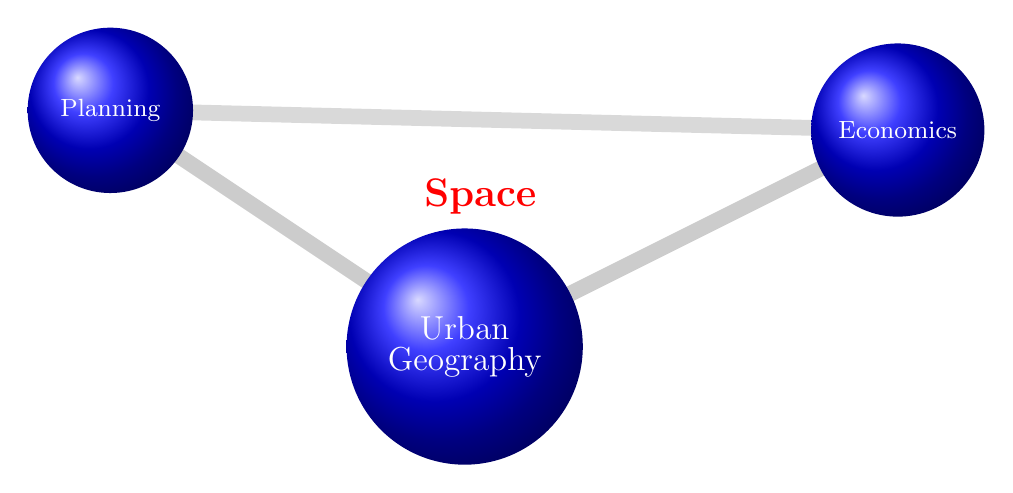
\begin{tikzpicture}{scale=.5}
% find color cotrol for ball. Tind way to stop line short of node
\coordinate (planning) at (-5,1);%PREFACE
\coordinate (economics) at (5,.75);%
 \coordinate (geography) at (-.5,-2); %history
\coordinate (finance) at (0,5); %

\draw [line width=2mm, black!15, ] (planning)--(economics);
\draw [line width=2mm, black!20, ] (geography)--(economics);
\draw [line width=2mm, black!20, ] (geography)--(planning);

%\draw [line width=2mm, black!25, ] (geography)--(finance);
%\draw [line width=2mm, black!20, ] (planning)--(finance);
%\draw [line width=2mm, black!20, ] (finance)--(economics);

\node [circle,shading=ball, minimum width=2.1   cm, white, align=center] (ball) at (planning) {Planning};
\node [circle,shading=ball, minimum width=2.2cm, white, align=center] (ball) at (economics) {Economics};
\node [circle,shading=ball, minimum width=3 . cm, white, align=center] (ball) at (geography)[text width=2cm] {\large Urban\\ Geography};

%\node [circle, shading=ball, minimum width=2.4cm, white, align=center] (ball) at (finance)[text width=2cm] {Finance};

\node at (-.3,-.1) [red] {\Large \textbf{Space}};
\end{tikzpicture}

Figure 1: The common concern of three fields
topic 

A simple economic insight -- that locational value gives rise to land rents -- provides an organizing principle for the three disciplines. Rent theory has a long history in economics, going back to thinkers such as Richard Cantillon (1680s-1734), François Quesnay (1694–1774), the marquis de Mirabeau (1715–1789) and Anne-Robert-Jacques Turgot (name physiocrat) and Adam Smith (1723-1790) and received its classic statement in Ricardo (1772-1823). Nearly contemporaneous thinker, Johann Heinrich  von Th\"unen (1783-1850) developed a planning model to guide the location of economic activities for an urban-agricultural society.  A version of that model  was reinvented in urban geography by XXX. Alonzo\footnote{We use a version of the well-established model of Alonso (1964), Muth (1969) and Mills (1967), and formalised by Wheaton (1974),}

We link the Alonzo model with more recent work on growth theory starting with Robert Solo's XXX and with the endogenous growth models of Lucas () and draw on Jane Jacobs's insight that endogenous urban growth  is. now driving economic development. Jacobs's insight is empirically supported by recent work in the complexity literature on urban scaling by XXXX ()




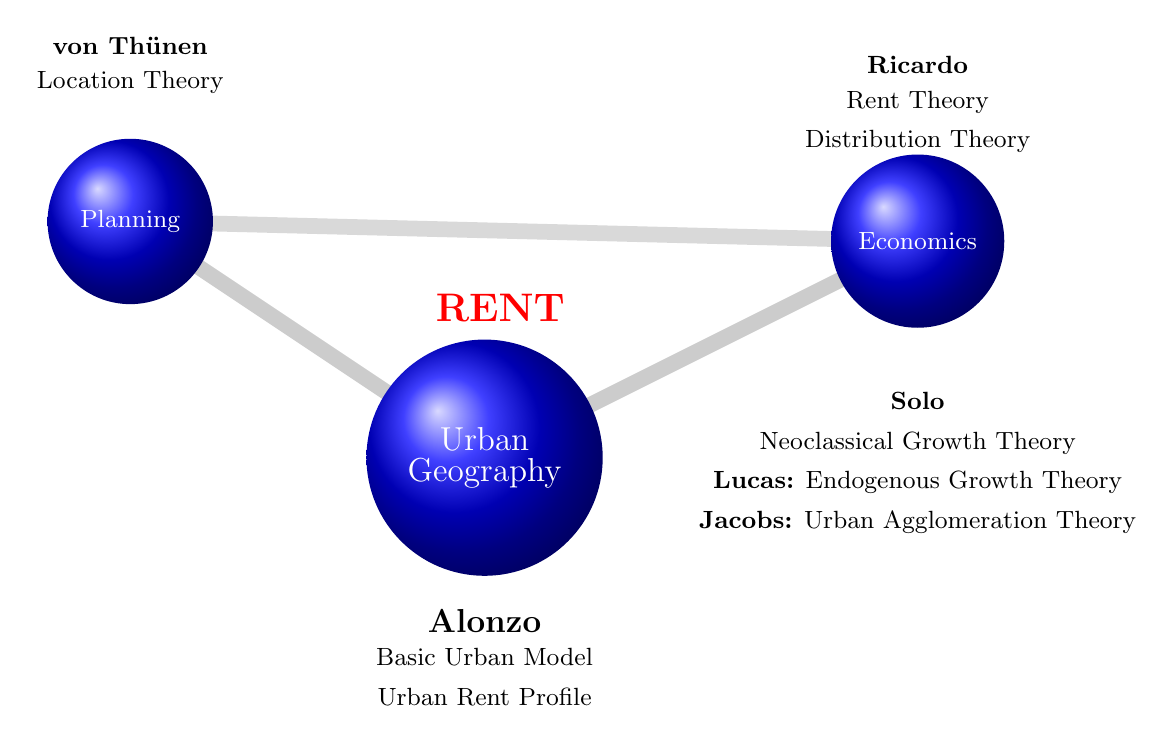
\begin{tikzpicture}{scale=.5}
% find color cotrol for ball. Tind way to stop line short of node
\coordinate (planning) at (-5,1);%PREFACE
\coordinate (economics) at (5,.75);%
 \coordinate (geography) at (-.5,-2); %history
\coordinate (finance) at (0,5); %

\draw [line width=2mm, black!15, ] (planning)--(economics);
\draw [line width=2mm, black!20, ] (geography)--(economics);
\draw [line width=2mm, black!20, ] (geography)--(planning);

%\draw [line width=2mm, black!25, ] (geography)--(finance);
%\draw [line width=2mm, black!20, ] (planning)--(finance);
%\draw [line width=2mm, black!20, ] (finance)--(economics);

\node [circle,shading=ball, minimum width=2.1   cm, white, align=center] (ball) at (planning) {Planning};
\node [circle,shading=ball, minimum width=2.2cm, white, align=center] (ball) at (economics) {Economics};
\node [circle,shading=ball, minimum width=3 . cm, white, align=center] (ball) at (geography)[text width=2cm] {\large Urban\\ Geography};

%\node [circle, shading=ball, minimum width=2.4cm, white, align=center] (ball) at (finance)[text width=2cm] {Finance};

\node at (-.3,-.1) [red] {\Large \textbf{RENT}};

% new stuff
\node at (planning) [above=2cm] {\textbf{von Th\"unen}};
\node at (planning) [above=1.5cm] {Location Theory};

\node at (economics) [above=2cm] {\textbf{Ricardo}};
\node at (economics) [above=1.5cm] {Rent Theory};
\node at (economics) [above=1.0cm] {Distribution Theory};

\node at (economics) [below=1.8cm] {\textbf{Solo}};
\node at (economics) [below=2.3cm] {Neoclassical Growth Theory};
\node at (economics) [below=2.8cm] {\textbf{Lucas:} Endogenous Growth Theory};
\node at (economics) [below=3.3cm] {\textbf{Jacobs:} Urban Agglomeration Theory};


\node at (geography) [below=1.8cm] {\textbf{\large Alonzo}};
\node at (geography) [below=2.3cm] {Basic Urban Model};
\node at (geography) [below=2.8cm] {Urban Rent Profile};
\end{tikzpicture}

Figure 3: space and value

Land rent was historically the basis of the wealth and political power of  the land-owning class in the era of the classical economists.


We further link the model of urban rents to emerging concerns about the financialization of the housing market. The key insight we offer is that the financialization  of the housing sector is a  form of rent-seeking that must have detrimental effects on urban development and on the well-being of urban residents.





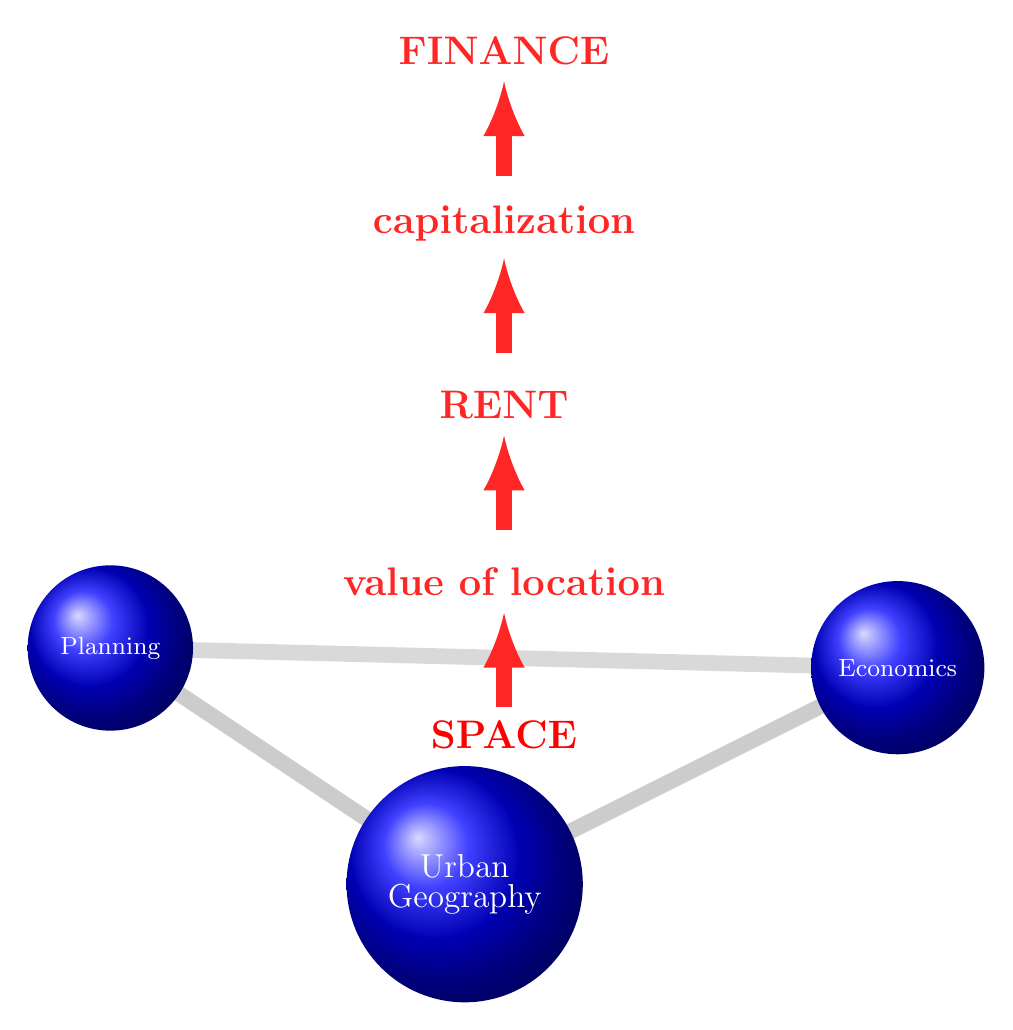
\begin{tikzpicture}{scale=.5}
% find color cotrol for ball. Tind way to stop line short of node
\coordinate (planning) at (-5,1);%PREFACE
\coordinate (economics) at (5,.75);%
 \coordinate (geography) at (-.5,-2); %history
\coordinate (finance) at (0,5); %

\draw [line width=2mm, black!15, ] (planning)--(economics);
\draw [line width=2mm, black!20, ] (geography)--(economics);
\draw [line width=2mm, black!20, ] (geography)--(planning);

%\draw [line width=2mm, black!25, ] (geography)--(finance);
%\draw [line width=2mm, black!20, ] (planning)--(finance);
%\draw [line width=2mm, black!20, ] (finance)--(economics);

\node [circle,shading=ball, minimum width=2.1   cm, white, align=center] (ball) at (planning) {Planning};
\node [circle,shading=ball, minimum width=2.2cm, white, align=center] (ball) at (economics) {Economics};
\node [circle,shading=ball, minimum width=3 . cm, white, align=center] (ball) at (geography)[text width=2cm] {\large Urban\\ Geography};

%\node [circle, shading=ball, minimum width=2.4cm, white, align=center] (ball) at (finance)[text width=2cm] {Finance};
\draw [line width=2mm, red!85, -latex ] (0, 7)--++(0,1.2)node[above=-.1] {\Large \textbf{FINANCE}};
\draw [line width=2mm, red!85, -latex ] (0, 4.75)--++(0,1.2)node[above=-.1] {\Large \textbf{capitalization}};
\draw [line width=2mm, red!85, -latex ] (0, 2.5)--++(0,1.2)node[above=-.1] {\Large \textbf{RENT}};
\draw [line width=2mm, red!85, -latex ] (0, .25)--++(0,1.2)node[above=-.1] {\Large \textbf{value of location}};
\node at (0,-.1) [red] {\Large \textbf{SPACE}};
\end{tikzpicture}



% \vspace {2cm}
% Figure 4 with finance

% \begin{tikzpicture}{scale=.5}
% % find color cotrol for ball. Tind way to stop line short of node
% \coordinate (planning) at (-5,1);%PREFACE
% \coordinate (economics) at (5,.75);%
%  \coordinate (geography) at (-.5,-2); %history
% \coordinate (finance) at (0,5); %

% \draw [line width=2mm, black!15, ] (planning)--(economics);
% \draw [line width=2mm, black!20, ] (geography)--(economics);
% \draw [line width=2mm, black!20, ] (geography)--(planning);

% \node at (-.3,2) [red] {\huge \textbf{RENT}};

% \draw [line width=3mm,  black!50,opacity=.5 ] (geography)--(finance);
% \draw [line width=2mm, black!20, ] (planning)--(finance);
% \draw [line width=2mm, black!20, ] (finance)--(economics);

% \node [circle,shading=ball, minimum width=2.1   cm, white, align=center] (ball) at (planning) {Planning};
% \node [circle,shading=ball, minimum width=2.2cm, white, align=center] (ball) at (economics) {Economics};
% \node [circle,shading=ball, minimum width=3 . cm, white, align=center] (ball) at (geography)[text width=2cm] {\large Urban\\ Geography};

% \node [circle, shading=ball, minimum width=2.4cm, white, align=center] (ball) at (finance)[text width=2cm] {Finance};


% \end{tikzpicture}

Summarizing the overall focus of the thesis,  we are concerned with the implication for urban development of growing rent extraction by the financial sector.  

\vspace {2cm}
Figure 4 with finance

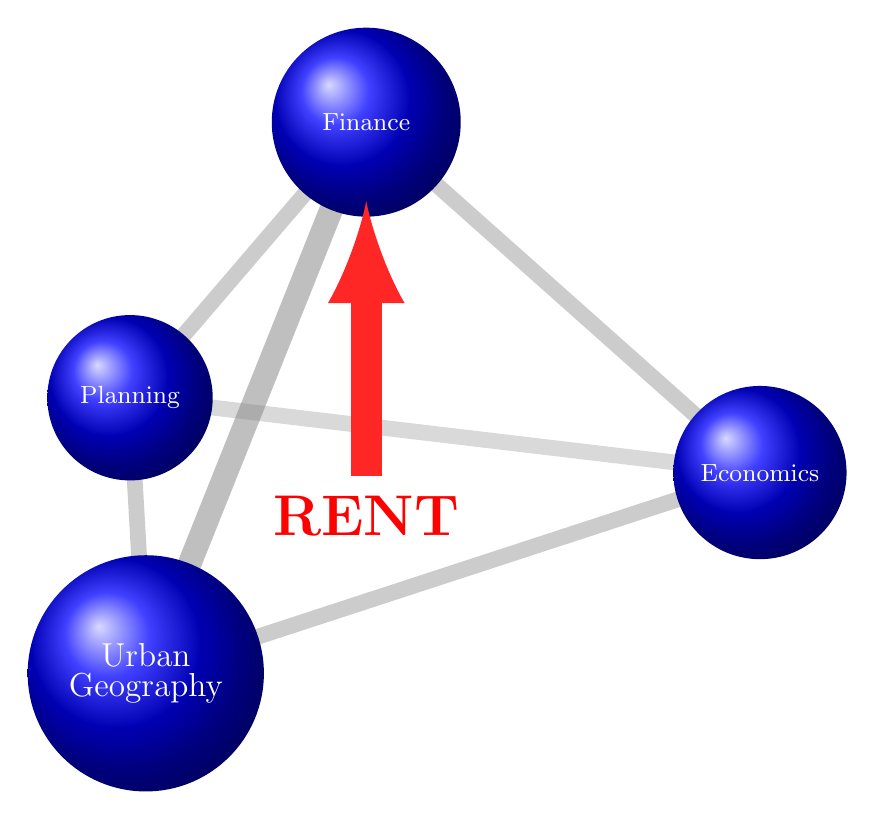
\begin{tikzpicture}{scale=.5}
% find color cotrol for ball. Tind way to stop line short of node
\coordinate (planning) at (-3,1.5);%PREFACE
\coordinate (economics) at (5,.55);%
 \coordinate (geography) at (-2.8,-2); %history
\coordinate (finance) at (0,5); %

\draw [line width=2mm, black!15, ] (planning)--(economics);
\draw [line width=2mm, black!20, ] (geography)--(economics);
\draw [line width=2mm, black!20, ] (geography)--(planning);

\node at (.0,0) [red] {\huge \textbf{RENT}};

\draw [line width=3mm,  black!50,opacity=.5 ] (geography)--(finance);
\draw [line width=2mm, black!20, ] (planning)--(finance);
\draw [line width=2mm, black!20, ] (finance)--(economics);

\node [circle,shading=ball, minimum width=2.1   cm, white, align=center] (ball) at (planning) {Planning};
\node [circle,shading=ball, minimum width=2.2cm, white, align=center] (ball) at (economics) {Economics};
\node [circle,shading=ball, minimum width=3 . cm, white, align=center] (ball) at (geography)[text width=2cm] {\large Urban\\ Geography};

\node [circle, shading=ball, minimum width=2.4cm, white, align=center] (ball) at (finance)[text width=2cm] {Finance};
\draw [line width=4mm, red!85, -latex ] (0, .5)--(0,4);


\end{tikzpicture}



\section{Document Overview}

\textbf{In chapter XXX}  we link classical rent theory, neoclassical production theory, neoclassical growth theory, the scaling literature, and urban spatial models.
To show how our model is directly connected with this broad collection of linked theories, we use the Cobb-Douglas function, which is used across this entire range of literature 

After we develop the mathematical description of the relationship among these will discuss  in more detail, rent theory and our contribution, scaling laws, ......  and other issues in the literature that draw on parts of this model and 

???  apply to the specific situation we're in why rent theory is related to discussions of exploitation why it might lead the inefficiencies, whether or not this links with other important models in the literature.

\textbf{In chapter XXX} we  provide a description of finacialization and show it is a a form of rent-seeking in the housing market and ?? the potential consequences of fiancialization in the housing market. 



\textbf{In chapter XXX} we  describe an illustrative agent-based model of the urban system. Most of the analysis of urban systems has employed analytical models with roots that go back to von Thunen () and more recently Alonzo. These models are extremely useful, but necessarily abstract from the concrete  and variable individual behaviour and  the details  of dynamics that make real cities path-dependent. XXX (Dawn) have shown that agent-based models can reproduce the features of the analytical models, at least in simple cases. 

ABMs can be run multiple times to produce distributions of expected outcomes, which makes them valuable in planning exercises. They also do not require  that we use a representative agent to make them tractable. Our model is intended to be elaborated  for such use. 

After we develop the mathematical description of the relationship among these will discuss in more detail, various relevant applications, and issues in the literature that draw on parts of this model and apply to the specific situation we're in why rent theory is related to discussions of exploitation why it might lead the inefficiencies, whether or not this links with other important models in the literature.


% Because we draw on a wide range of methods and literatures, we discuss the relevant literature and  methodologies in the chapters where they apply 


\chapter{Background} \label{chapter-background}
The focus of this thesis on a topic. that falls in the overlap  between least three academic  disciplines, Economics, Urban Geography, and Planning. The central and shared concern in this area is with geographic space.

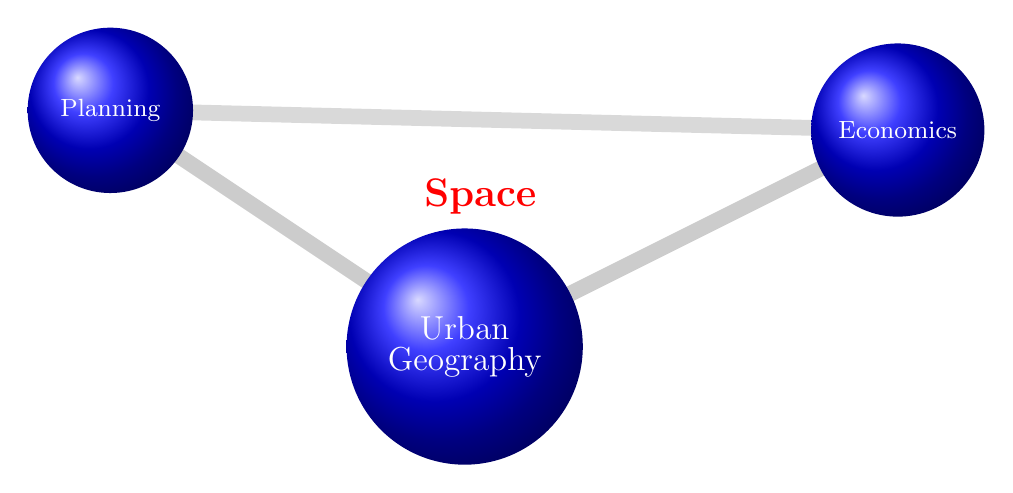
\begin{tikzpicture}{scale=.5}
% find color cotrol for ball. Tind way to stop line short of node
\coordinate (planning) at (-5,1);%PREFACE
\coordinate (economics) at (5,.75);%
 \coordinate (geography) at (-.5,-2); %history
\coordinate (finance) at (0,5); %

\draw [line width=2mm, black!15, ] (planning)--(economics);
\draw [line width=2mm, black!20, ] (geography)--(economics);
\draw [line width=2mm, black!20, ] (geography)--(planning);

%\draw [line width=2mm, black!25, ] (geography)--(finance);
%\draw [line width=2mm, black!20, ] (planning)--(finance);
%\draw [line width=2mm, black!20, ] (finance)--(economics);

\node [circle,shading=ball, minimum width=2.1   cm, white, align=center] (ball) at (planning) {Planning};
\node [circle,shading=ball, minimum width=2.2cm, white, align=center] (ball) at (economics) {Economics};
\node [circle,shading=ball, minimum width=3cm, white, align=center] (ball) at (geography)[text width=2cm] {\large Urban\\ Geography};

%\node [circle, shading=ball, minimum width=2.4cm, white, align=center] (ball) at (finance)[text width=2cm] {Finance};

\node at (-.3,-.1) [red] {\Large \textbf{Space}};
\end{tikzpicture}

Figure 1: The common concern of three fields
topic 

A simple economic insight -- that locational value gives rise to land rents -- provides an organizing principle for the three disciplines. Rent theory has a long history in economics, going back to thinkers such as Richard Cantillon (1680s-1734), François Quesnay (1694–1774), the marquis de Mirabeau (1715–1789) and Anne-Robert-Jacques Turgot (name physiocrat) and Adam Smith (1723-1790) and received its classic statement in Ricardo (1772-1823). Nearly contemporaneous thinker, Johann Heinrich  von Th\"unen (1783-1850) developed a planning model to guide the location of economic activities for an urban-agricultural society.  A version of that model  was reinvented in urban geography by XXX. Alonzo\footnote{We use a version of the well-established model of Alonso (1964), Muth (1969) and Mills (1967), and formalised by Wheaton (1974),}

We link the Alonzo model with more recent work on growth theory starting with Robert Solo's XXX and with the endogenous growth models of Lucas () and draw on Jane Jacobs's insight that endogenous urban growth  is. now driving economic development. Jacobs's insight is empirically supported by recent work in the complexity literature on urban scaling by XXXX ()




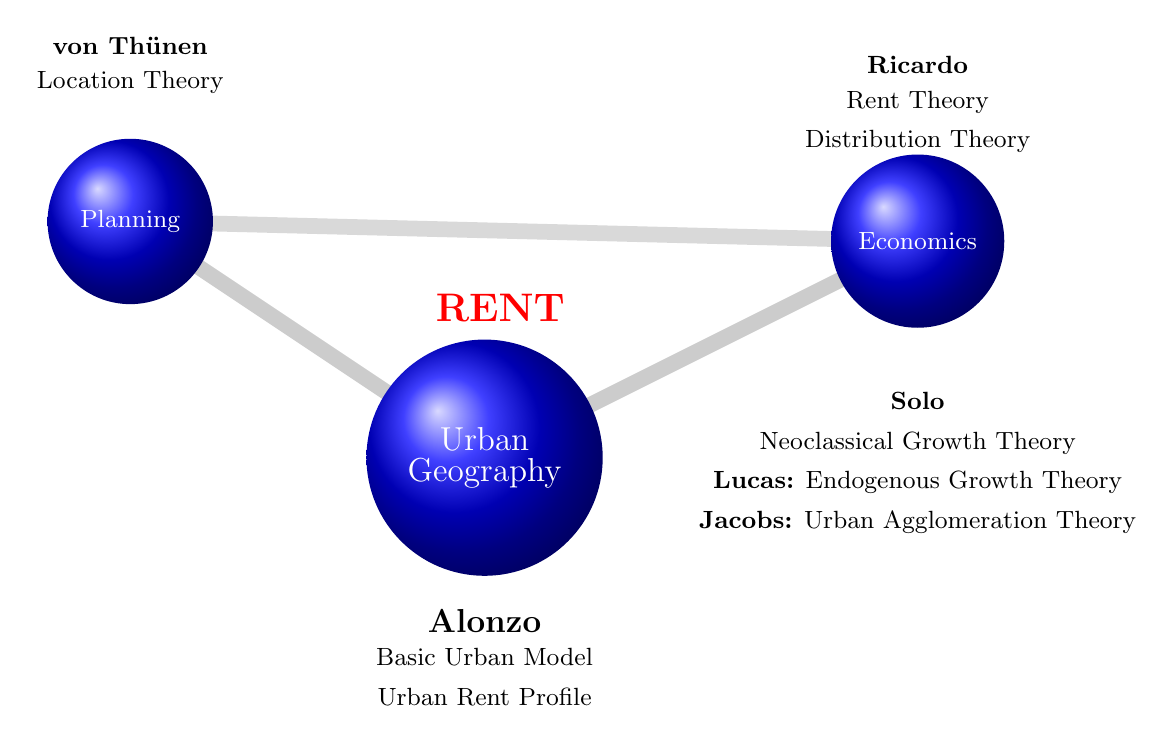
\begin{tikzpicture}{scale=.5}
% find color cotrol for ball. Tind way to stop line short of node
\coordinate (planning) at (-5,1);%PREFACE
\coordinate (economics) at (5,.75);%
 \coordinate (geography) at (-.5,-2); %history
\coordinate (finance) at (0,5); %

\draw [line width=2mm, black!15, ] (planning)--(economics);
\draw [line width=2mm, black!20, ] (geography)--(economics);
\draw [line width=2mm, black!20, ] (geography)--(planning);

%\draw [line width=2mm, black!25, ] (geography)--(finance);
%\draw [line width=2mm, black!20, ] (planning)--(finance);
%\draw [line width=2mm, black!20, ] (finance)--(economics);

\node [circle,shading=ball, minimum width=2.1   cm, white, align=center] (ball) at (planning) {Planning};
\node [circle,shading=ball, minimum width=2.2cm, white, align=center] (ball) at (economics) {Economics};
\node [circle,shading=ball, minimum width=3cm, white, align=center] (ball) at (geography)[text width=2cm] {\large Urban\\ Geography};

%\node [circle, shading=ball, minimum width=2.4cm, white, align=center] (ball) at (finance)[text width=2cm] {Finance};

\node at (-.3,-.1) [red] {\Large \textbf{RENT}};

% new stuff
\node at (planning) [above=2cm] {\textbf{von Th\"unen}};
\node at (planning) [above=1.5cm] {Location Theory};

\node at (economics) [above=2cm] {\textbf{Ricardo}};
\node at (economics) [above=1.5cm] {Rent Theory};
\node at (economics) [above=1.0cm] {Distribution Theory};

\node at (economics) [below=1.8cm] {\textbf{Solo}};
\node at (economics) [below=2.3cm] {Neoclassical Growth Theory};
\node at (economics) [below=2.8cm] {\textbf{Lucas:} Endogenous Growth Theory};
\node at (economics) [below=3.3cm] {\textbf{Jacobs:} Urban Agglomeration Theory};


\node at (geography) [below=1.8cm] {\textbf{\large Alonzo}};
\node at (geography) [below=2.3cm] {Basic Urban Model};
\node at (geography) [below=2.8cm] {Urban Rent Profile};
\end{tikzpicture}

Figure 3: space and value

Land rent was historically the basis of the wealth and political power of  the land-owning class in the era of the classical economists.


We further link the model of urban rents to emerging concerns about the financialization of the housing market. The key insight we offer is that the financialization  of the housing sector is a  form of rent-seeking that must have detrimental effects on urban development and on the well-being of urban residents.





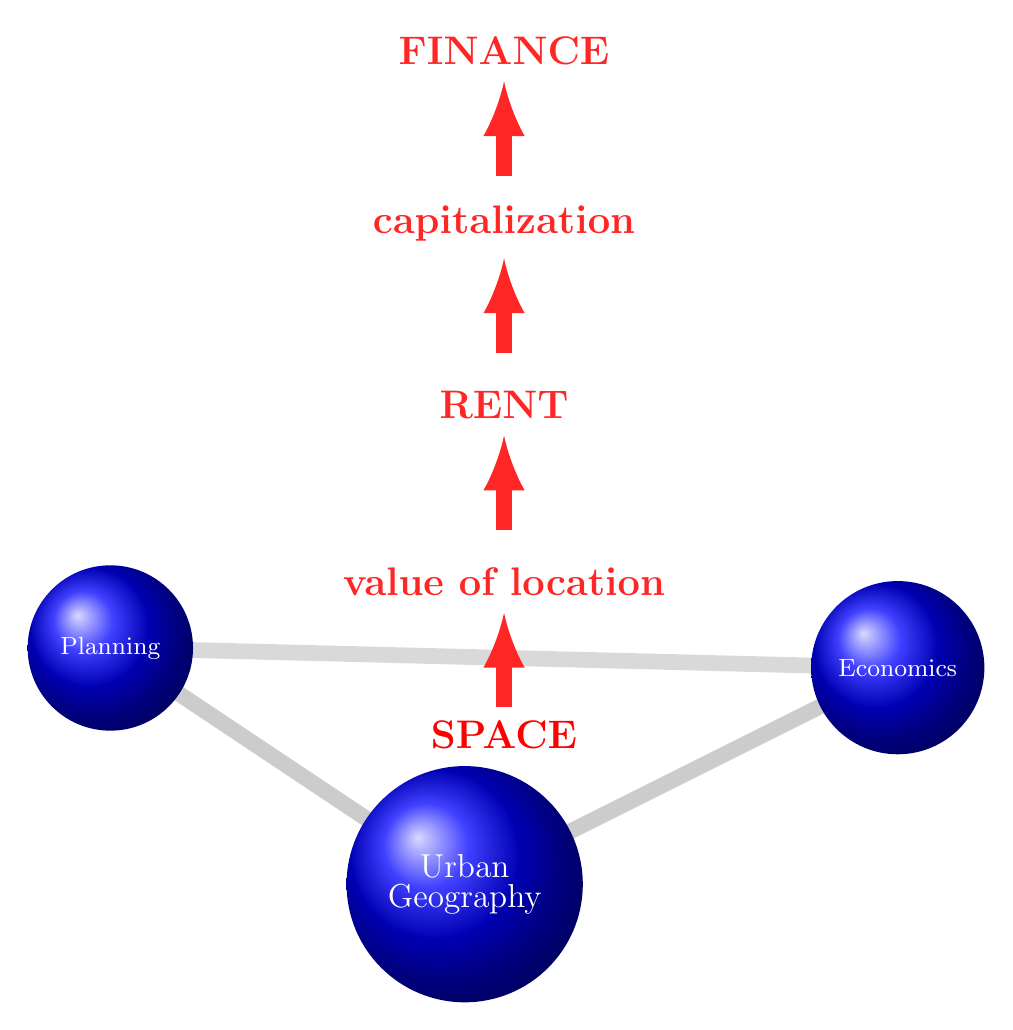
\begin{tikzpicture}{scale=.5}
% find color cotrol for ball. Tind way to stop line short of node
\coordinate (planning) at (-5,1);%PREFACE
\coordinate (economics) at (5,.75);%
 \coordinate (geography) at (-.5,-2); %history
\coordinate (finance) at (0,5); %

\draw [line width=2mm, black!15, ] (planning)--(economics);
\draw [line width=2mm, black!20, ] (geography)--(economics);
\draw [line width=2mm, black!20, ] (geography)--(planning);

%\draw [line width=2mm, black!25, ] (geography)--(finance);
%\draw [line width=2mm, black!20, ] (planning)--(finance);
%\draw [line width=2mm, black!20, ] (finance)--(economics);

\node [circle,shading=ball, minimum width=2.1   cm, white, align=center] (ball) at (planning) {Planning};
\node [circle,shading=ball, minimum width=2.2cm, white, align=center] (ball) at (economics) {Economics};
\node [circle,shading=ball, minimum width=3cm, white, align=center] (ball) at (geography)[text width=2cm] {\large Urban\\ Geography};

%\node [circle, shading=ball, minimum width=2.4cm, white, align=center] (ball) at (finance)[text width=2cm] {Finance};
\draw [line width=2mm, red!85, -latex ] (0, 7)--++(0,1.2)node[above=-.1] {\Large \textbf{FINANCE}};
\draw [line width=2mm, red!85, -latex ] (0, 4.75)--++(0,1.2)node[above=-.1] {\Large \textbf{capitalization}};
\draw [line width=2mm, red!85, -latex ] (0, 2.5)--++(0,1.2)node[above=-.1] {\Large \textbf{RENT}};
\draw [line width=2mm, red!85, -latex ] (0, .25)--++(0,1.2)node[above=-.1] {\Large \textbf{value of location}};
\node at (0,-.1) [red] {\Large \textbf{SPACE}};
\end{tikzpicture}



% \vspace {2cm}
% Figure 4 with finance

% \begin{tikzpicture}{scale=.5}
% % find color cotrol for ball. Tind way to stop line short of node
% \coordinate (planning) at (-5,1);%PREFACE
% \coordinate (economics) at (5,.75);%
%  \coordinate (geography) at (-.5,-2); %history
% \coordinate (finance) at (0,5); %

% \draw [line width=2mm, black!15, ] (planning)--(economics);
% \draw [line width=2mm, black!20, ] (geography)--(economics);
% \draw [line width=2mm, black!20, ] (geography)--(planning);

% \node at (-.3,2) [red] {\huge \textbf{RENT}};

% \draw [line width=3mm,  black!50,opacity=.5 ] (geography)--(finance);
% \draw [line width=2mm, black!20, ] (planning)--(finance);
% \draw [line width=2mm, black!20, ] (finance)--(economics);

% \node [circle,shading=ball, minimum width=2.1   cm, white, align=center] (ball) at (planning) {Planning};
% \node [circle,shading=ball, minimum width=2.2cm, white, align=center] (ball) at (economics) {Economics};
% \node [circle,shading=ball, minimum width=3 . cm, white, align=center] (ball) at (geography)[text width=2cm] {\large Urban\\ Geography};

% \node [circle, shading=ball, minimum width=2.4cm, white, align=center] (ball) at (finance)[text width=2cm] {Finance};


% \end{tikzpicture}



\vspace {2cm}
Figure 4 with finance

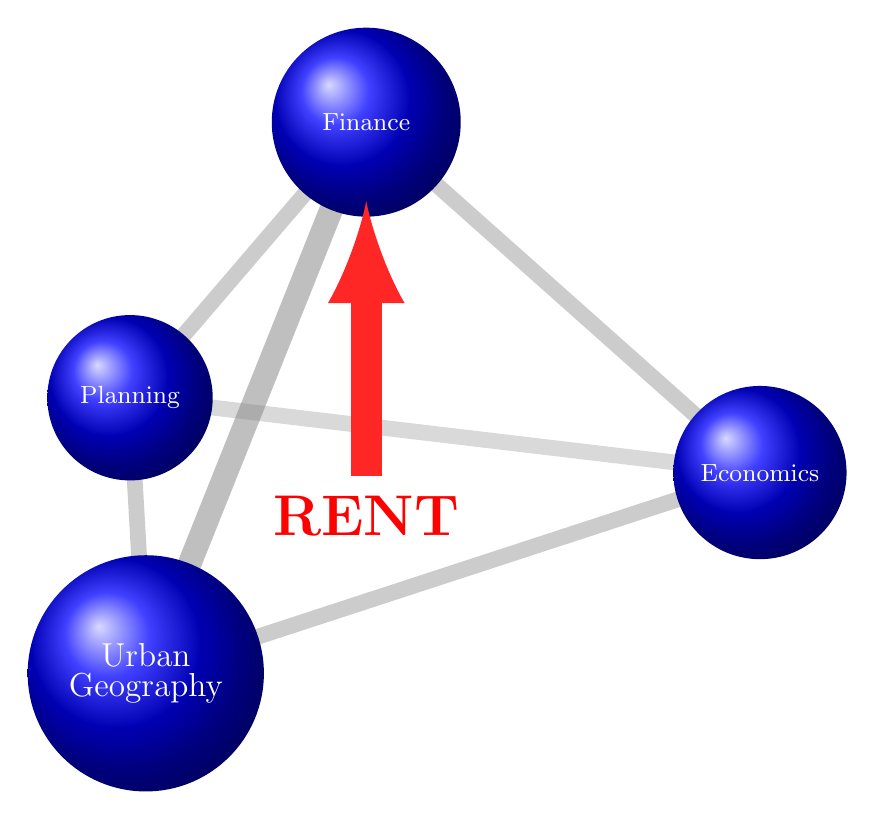
\begin{tikzpicture}{scale=.5}
% find color cotrol for ball. Tind way to stop line short of node
\coordinate (planning) at (-3,1.5);%PREFACE
\coordinate (economics) at (5,.55);%
 \coordinate (geography) at (-2.8,-2); %history
\coordinate (finance) at (0,5); %

\draw [line width=2mm, black!15, ] (planning)--(economics);
\draw [line width=2mm, black!20, ] (geography)--(economics);
\draw [line width=2mm, black!20, ] (geography)--(planning);

\node at (.0,0) [red] {\huge \textbf{RENT}};

\draw [line width=3mm,  black!50,opacity=.5 ] (geography)--(finance);
\draw [line width=2mm, black!20, ] (planning)--(finance);
\draw [line width=2mm, black!20, ] (finance)--(economics);

\node [circle,shading=ball, minimum width=2.1   cm, white, align=center] (ball) at (planning) {Planning};
\node [circle,shading=ball, minimum width=2.2cm, white, align=center] (ball) at (economics) {Economics};
\node [circle,shading=ball, minimum width=3cm, white, align=center] (ball) at (geography)[text width=2cm] {\large Urban\\ Geography};

\node [circle, shading=ball, minimum width=2.4cm, white, align=center] (ball) at (finance)[text width=2cm] {Finance};
\draw [line width=4mm, red!85, -latex ] (0, .5)--(0,4);


\end{tikzpicture}

\chapter{Antecedents of modern Urban Rent theory}
In this chapter, we link classical rent theory, neoclassical production theory, neoclassical growth theory, the scaling literature, and urban spatial models. 

%We use the Cobb-Douglas function %, which is used to cross this entire range of literature to illustrate each link and to show how our model is directly connected with this broad collection of linked theories. 
%The Cobb-Douglas function is a production function, expressing the output produced, in terms of inputs such as labour and capital.
%Our model connects to the results in this chapter at four points:



\section{Classical theories of production and distribution}
INTRODUCE RICARDO, CLASSICAL THEORIES - OR RESTRUCTURE AS AN INTRO SENTENCE.
MAYBE REVIEW SOME ALTERNATIVES/FRAME RICARDO
 % \subsection{Ricardo}

 The core social question that Ricardo addressed was who gets the surplus. % The question was pressing because it appeared that landlords were capturing the surplus without contributing to production while many of those who worked that land were very poor. 
Ricardo uses his model to explain the distribution of the product of the earth among the “three classes of the community” which is to say, to the owners of land, labour, and capital. 

% going back to the Physiocrates. 
% The physiocratic school of economics was the first to see labor as the sole source of value but, for the physiocrats, in the context of the prevalent European rural society of the time, only agricultural labor created a surplus. % actually? % detail for it was ag economy This was the theory? also the french enginneers- detail for start of math/calc-..
%The canonical reference for only agricultural labour mattering? For the definition of rent?

%Ricardo's famous 1815 discussion of capital and  land rent \footnote{ %\href{http://la.utexas.edu/users/hcleaver/368/368RicardoOnCornLaws.html}{An Essay on the Influence of a low Price of Corn on the Profits of Stock}; 
%showing the Inexpediency of Restrictions on Importation: With Remarks on Mr Malthus' Two Last Publications: "An Inquiry into the Nature and Progress of Rent," and "The Grounds of an Opinion on the Policy of restricting the Importation of Foreign Corn"} provides the canonical reference. 
% We haven't introduced this model or what kind of thing it is.
The concept of rent in economics must be distinguish from the common use of the term to mean the payment paid to rent a property. 

In the classical tradition, rent is the value landowners claimed for the use of their land. Ricardo defines rent strictly in this way, saying ``By rent I always mean the remuneration given to the landlord for the use of the original power of the land\footnote{'' David Ricardo corn laws note 7.}. % explan that ricardo used this as a formal definition of the term. he ....

For Ricardo, and for the classical economics in general however, land rent, is a kind of surplus value, that is an amount available after the costs of production have been paid, the term rent came to be used interchangeably with this more general concept in much of the classical work on rent.
%and the term rent has been used in a more general sense to other kinds of surplus value, as well as land rents 
as Saunders says in 1902, ``Of the concrete forms of income that have usually been classed as surplus, the rent of land was the earliest to be defined; and so prominent a position has been given to it that the terms "rent" and "surplus" have come to be used interchangeably.'' \footnote{Rent in Modern Economic Theory: An Essay in Distribution Author(s): Alvin Saunders Johnson, Publications of the American Economic Association, Nov., 1902, 3rd Series, Vol. 3, No. 4 (Nov., 1902), pp. 1-129}. 
So for instance professional sports players' income, above the opportunity cost they could get working at another position, is rent they capture for their skill. 

The classical idea of rent and rent can be illustrated with the story of a carter who picks up vegetables at the farm gate and transports them into town, where he sells them to a  storekeeper. %He pays the farmer at one end of the trip and is paid at the other. 
For simplicity, assume all farmers have the same cost of production, and the carters pay the farmer the farm gate price at the farm and receive the merchant price in town. 

\begin{figure}
    \begin{center}
     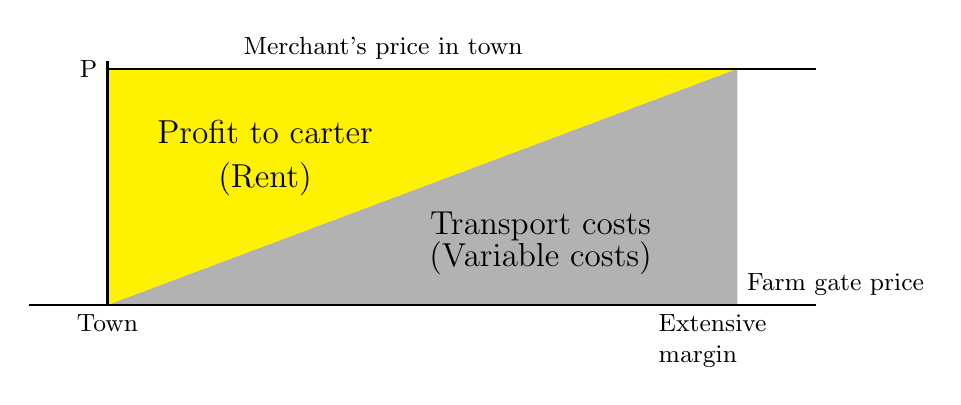
\begin{tikzpicture}[domain=0:2]
%\draw[thick,color=gray,step=.5cm, dashed] (-0.5,-.5) grid (3,3);
%\draw[line width=.01, green ] (0,0) -- (10,0) node[right  ] {Distance};
\node at (1,0) [below] {Town};
\fill[yellow]  (1,0) --(9,3)--(1,3) --cycle;
\fill[gray!60] (9,3) --(1,0)--(9,0) --cycle;

\draw[thick ] (1,3)node[left]{P}  -- (10,3);\node at (4.5,3)[above ] {Merchant's price in town} ;
\draw[thick ] (0,0)  -- (10,0); 

%\draw[thick,color=red] (1.5,0) -- (1.5,1) node[below right] {Fixed cost} -- (1.5,1.5) --(10,3.25)node[above left] {total cost};
\draw[thick] (1,0) -- (1,3.1) ;
\node[below,text width=2cm]at (9,0) {Extensive margin};
%\draw[ultra thick, blue,<-> ] (3,1.8) -- (3,2.5)node[left] {annual rent at a} -- (3,3) ; 
\node at (9,0)[above right] {Farm gate price};
\node  at (6.5,1){\large Transport costs};
\node  at (6.5,.6){\large (Variable costs)};
\node  at (3.,2.2){\large Profit to carter};
\node  at (3.,1.6){\large (Rent)};
\end{tikzpicture} 
    \caption{Transport costs, the yellow area, take a share of the profit for vegetables sold in the town}
    \label{fig:rent_ricardo}
    \end{center}
\end{figure}

In the figure \ref{fig:rent_ricardo}, total transport costs are shown as the yellow area. The area below the yellow triangle is profit for the carter. The carter makes a `profit' on the trip to the farm nearest to town, but there is a farm so far out  that transport costs eat up all the profit on the trip. That is as far as the carter will go\footnote{Note the similarity with Alonzo's urban model, illustrated in Fig \ref{Fig:rent_alonzo}.}. Ricardo termed this point the `extensive margin', the point at which there is no value for farming for the town. It is the limit for this use, and the profit there is zero. If the price goes up, the extensive margin moves out, and more land comes into production.

The land rent declines with distance from the town,\footnote{It also declines for less fertile land, where there is a higher cost of production.} At the extensive margin the land rent falls to zero. Even fertile land beyond the extensive margin will not be farmed because the product cannot be transported to market at a profit.\footnote{This simple example assumes that the land is uniformly productive and that there is only one product that can be marketed. Johann Heinrich von Th\"unen, in The Isolated state (Der isolierte Staat (1826)), provide a more complex analysis based on the same principles.} Transportation costs and the price of produce in town determine the size of the  rent triangle and therefore the amount of rent captured by the land-owning class.\footnote{The debate about the  `Corn Laws" that Ricardo  was engaged in was about whether Britain would allow wheat form Canada and Australia to enter, reducing the price of wheat and therefore reducing the income and influence of the land-owning class.} 

Together these two triangles/areas represent the ``produce of the earth'', but only the lower triangle is net income\footnote{ Termed the `\textit{produit net}' by the Physiocrats}. In modern supply and demand analysis it would be recognized as `producer surplus', the difference between what a producer gets for a good and what they would be willing to accept.

In Ricardo's case: the land owner delivers the grain to market and receives the merchant price. The profit is what the landowner could claim for the privilege of using the land %The profit now accrues to the landowner, and we call it land rent. For Ricardo, it was obvious that the land-owning class captured the land rent.
\footnote{In the modern economy, agricultural land rents may be captured by corporations,  either by owning the land or by controlling the supply chain.}  Landlord income is a locational land rent that exists because of the land's proximity to the market. 
 

%\subsection{A more explicit treatment}

Ricardo expounded a theory of land rent. While he did not write down a formal production function as later neoclassical theorists would, modern neoclassical production theory can be seen as having one of its origins in his work on classical economic theory.
In modern notation, Ricardo's model can be written:

\begin{equation} 
Y=F(K,L,N).
\label{Eqn:Prod1}
\end{equation} 

where $K$ is capital, $L$ is labour and $N$  is the natural resource  land.\footnote{This makes it a three factor model of production (cite us/lit) In principle any number of factors can be included.}  
Ricardo does not specify a functional form, but, %like mathematical neoclassical economists, 
he does assume diminishing returns to all factors. The landlord  receives the surplus generated by the land and the rest of the value of production goes to labour and to any capital employed in improving the land. 

The value of the land is the present discounted value of the surplus it generates, that is what it would be worth paying now, to capture the future rents from that land.


\subsection{Marx}


%Ricardo, agreeing with Malthus, essentially assumes that the wage is  just sufficient to reproduce the labouring class.\footnote{``In the natural advance of society, the wages of labour will have a tendency to fall, as far as they are regulated by supply and demand; for the supply of labourers will continue to increase at the same rate, while the demand for them will increase at a slower rate.''} He then explains the distribution of the fruits of labour on the land among the main classes of the economy.

 Marx shifted attention to the manufacturing economy in which the owners contributed the machinery, buildings, and even working capital to fund the workers until the product can be sold. %This contribution must be accumulated from their profits in the preceding cycle of production,  and has to be reinvested once the revenues of the current round have come in and the bills have been paid. Marx actually describes a circuit of capital from its form as money to its form as physical capital. 
As in Ricardo, however, labour is in surplus and capital is scarce. As in Ricardo the scarce factor owned by a special class - now the capitalists, is able to appropriate the is able to capture the surplus value. %Like Ricardo,  Marx saw the appropriation of surplus as without moral justification. 

Marx pointed to a new dynamic in capitalist systems - that productive capital is not fixed as land is, but  expands as surplus is reinvested. %He famously suggested that the expansion will eventually outrun the expansion of demand and the rate of return will fall, leaving capitalists unwilling to invest. % and creating a crisis. 

Marx gives the statement of the dynamic quality of the surplus
- work linking urban rents to the dynamic quality of the surplus in the urban system is in that tradition 
- how does the generative surplus gets distributed, its dynamics/the dynamics of the surplus. 
 
\subsection{Henry George} 


  Henry George, an influential American political economist,\footnote{Progress and Poverty: An Inquiry into the Cause of Industrial Depressions and of Increase of Want with Increase of Wealth: The Remedy (1879) book by social theorist and economist Henry George.}  returned to land rent with a new insight based on the emergence of the capitalist city: ``With the growth of population, land grows in value, and the men who work it must pay more for the privilege.'' For George the owners of urban land extract surplus in exactly the same way that owners of agricultural land in Ricardo's analysis. Where Marx saw the extravagant productivity of capital as the source of capitalist crises, George saw the extraction of wealth by land speculators as the mechanism that would bring on crises.
  
  Since land rent is not created by its owners, George argued that land rent should be seen as a social income - that it could be used to pay for all the needs of the community. The clearest statement of this view is found in Progress and Poverty: "We must make land common property." The same view was expressed by the Physiocrats who concluded  that ``ground rents'' should be the source of most or all taxes. They defined ground rent as that portion of all rent which is attributable only to the size and location of the parcel. George's analysis the `single tax' movement, which sought to shift all taxation to land  and resource rents.   
  
  In 1977, Joseph Stiglitz  showed, using a standard urban model, identified the conditions in which Henry George's "single tax" is  the only tax necessary to finance public expenditures.\footnote{Arnott, Richard J.; Joseph E. Stiglitz (November 1979). "Aggregate Land Rents, Expenditure on Public Goods, and Optimal City Size" (PDF). Quarterly Journal of Economics. 93 (4): 471–500. doi:10.2307/1884466. JSTOR 1884466. S2CID 53374401 }   The logic is fairly simple: if the public good increases productivity or the attractiveness of a city, attracting more people or businesses, land rents rise, and investment in the public good should proceed until the marginal cost of the public good is equal to the increase in land rent it brings. The result is now called the `Henry George theorem.'



The classical economists agreed that rents are unearned income. They did not emphasize, as George did, that land rents arise from labour's proximity to urban population and production.\footnote{To be fair, it was not lack of understanding, that the omission reveals, but rather lack of interest in explicitly examining urban land rent from residential or even industrial purposes.}% Ricardo von Thunen, Marx, Cantillon all grasped the notion of proximity to the market as part of the source land rent. The discussions seem to not gone farther than discussions of diffeerential and rents, however.  I just am not aware of them explicitly examining urban land rent for residential or even industrial purposes. 

%The need to be near a market or prodduction center is easily seen by considering a population at the carrying capacity of the land with individuals supporting themselves using purely local resources. There can be no land rent in this case. If a city rises that must be supplied from those still on the land, land close enough to the city will generate land rent. The value of the land is created by proximity to the city.



%  no separate and comprehensive data are provided on the amounts of land rents and subsoil rents charged and earned, because they are not officially regarded as part of value-added, and consequently are not included in the calculation of GDP (except for the value of productive lease contracts)     https://en.wikipedia.org/wiki/Differential_and_absolute_ground_rent#Rent_in_macro-economics    \href{https://en.wikipedia.org/wiki/Differential_and_absolute_ground_rent#Rent_in_macro-economics}{Wikipediat article on differential rent}

Stiglits is linking the capture of urban rents to productivity.

  \subsection{John Bates Clark and neoclassical distribution theory}
  Classical theories of distribution showed that ownership of a scarce and non-produced factor, land, was the  basis of rent extraction by the class of landowners. Profits were a bit puzzling in this context - Capital also earns its return from scarcity. Marshall pointed out, however, that scarcity profits (i.e., rent) would normally be competed away  as entrepreneurs entered the market in pursuit of those `excess' profits. He used the term `pseudo-rents' for these unearned but temporary incomes.\footnote{Alvin Saunders Johnson. Rent in Modern Economic Theory: An Essay in Distribution. AEA 3rd Series, Vol. 3, No. 4 (Nov., 1902), pp. 1-129 (129 pages)}

 John Bates Clark was one of the pioneers of marginalism and the neoclassical theory of  distribution.  The marginalist approach emphasized the rational decisions of economic agents in allocating their resources would lead them to allocate resources according to the value of the marginal product of the resource in production.  Initially a socialist like George, by 1986 he was praising the dynamical process of competition partly in opposition to the single tax movement George had initiated.  His (1891) ``Distribution as Determined by a Law of Rent,'' argued that, given  competition and homogeneous factors of production labor and capital, the division of the social product will be according to the productivity of the last (or marginal) physical input of units of labor and capital.\footnote{Responding to the "indictment that hangs over society" that it involves "exploiting labor," Clark wrote:

    It is the purpose of this work (his 1899 'Distribution of Wealth) to show that the distribution of the income of society is controlled by a natural law, and that this law, if it worked without friction, would give to every agent of production the amount of wealth which that agent creates. However wages may be adjusted by bargains freely made between individual men (i.e., without labor unions and other "market imperfections", the rates of pay that result from such transactions tend, it is here claimed, to equal that part of the product of industry which is traceable to the labor itself; and however interest (i.e., profit) may be adjusted by similarly free bargaining, it naturally tends to equal the fractional product that is separately traceable to capital.} 
 
Clark's analysis of income distribution does not contradict the classical view of rents, it simply displaces the analysis to the point where a competitive equilibrium prevails, and shifts attention away from the distribution of land rents. Rents are not earned by the marginal unit of land and  





\section{Neoclassical production theory}
The concept of a production function used by increasingly mathematical neoclassical economists and  rapidly developing statistical techniques  naturally led to attempts to identify the precise functional form that would describe the contributions of labour, capital, and income to output.
 
Mathematician Charles Cobb and Economist Paul Douglas came up with a specific and very convenient functional form\footnote{Cobb, C. W.; Douglas, P. H. (1928). "A Theory of Production"  American Economic Review. 18 (Supplement): 139–165. JSTOR 1811556. Retrieved 26 September 2016. The function had apparently previously been used by Knut Wicksell, Philip Wicksteed, and L\'eon Walras.} that captured much of what economists were talking about. The function is just a generalized arithmetic mean:
 
 \[Y=AK^\alpha L^\beta\]
 where $A$ is a constant scale factor, commonly called `Total Factor Productivity. This function becomes the workhorse of neoclassical growth theory in the second half  of the 20th century. Our urban model is a direct heir of those developments.

%The Cobb Douglas function has several convenient features. One is that the sum of the coefficents tells us the degree of returns to scale. If $\alpha+\beta = 1$, we have constant returns to scale,

%Another is that the coefficients of the factors, $\alpha$  and $\beta$ turn out to be the elasticities of output with respect to capital and labour respectively as well as the income share of the factor. These made it relatively easy for economists to combine national data on labour and capital stocks or income with output to test the model.

The Cobb–Douglas form was developed and almost immediately tested against statistical evidence in the USA by Cobb and Douglas between 1927–1947. It was  their widely circulated empirical work seems to have permanently associated this simple function with Cobb and Douglas for economists.

The Cobb-Douglas form captured  important regularities in the cross-sectional national data,\footnote{ A 2021 meta-analysis of 3186 estimates concluded that "the weight of evidence accumulated in the empirical literature emphatically rejects the Cobb-Douglas specification."Gechert, Havranek, Irsova, Kolcunova (2021), "Measuring capital-labor substitution: The importance of method choices and publication bias", Review of Economic Dynamics, doi:10.1016/j.red.2021.05.003, S2CID 236400765. More sophisticated models  such as the CES and translog functions have been developed  since.} 
but the estimates soon showed a systematic bias with time series. Essentially the value of the $A$ seemed to rise over time. Something that was not captured in the initial model  contributed to productivity over time: 
 \[Y=A(t)K^\alpha L^\beta\]



\section{MOVE SECTION BRINGING PRODUCTIVE LAND BACK IN Neoclassical production}

Ricardo analysis of land can be thourght of as:

\begin{equation} 
Y=F(K,L,N).
\label{Eqn:Prod1}
\end{equation} 
where $K$ is capital, $L$ is labour and $N$  is the natural resource  land.

Most modern neoclassical treatments of production have the same basic structure of the production function, but they simplify by omitting land: 

\begin{equation} 
Y=F(K,L).
\label{Eqn:Prod1}
\end{equation} 

    
Which makes sense for a number of reasons. The economy has shifted from agriculture to industry as well as
%Leaving land out of the model makes sense for a variety of reasons. 
And, according to the Ricardian theory, rent is a surplus above cost. It does not, therefore enter into price. Land is a fixed factor for society as a whole that is not consumed in  the process of production.  Furthermore, neoclassical treatments of production focus price determination based on the cost of the last unit used, the marginal  unit of input, while rents are generated on all of the inframarginal units, those units used earlier, which are more productive. The marginal unit of land generates no rents. In neoclassical analysis, the rents disappeared from view for this reason. This difference is at the heart of the distinction between classical and neoclassical economic theory. 

%John B. Davis. Ricardo's Theory of Profit and the Third Edition of the \textit{Principles}. Journal of the History of Economic Thought, 15, Spring 1993. °1993 by the History of Economic Society.
%``Questions arise, however, when one turns to exchange between a sector paying rent and one not.'' The Principles tells us that as cultivation is extended and exchange increases, profits fall while rents increase. 

Leaving land out, however, creates a problem in  the neoclassical growth theories we will examine below. Under the assumption of perfectly competitive goods and factors markets as well as marginal productivity pricing of capital and labor, neoclassical growth requires technical change to be generated outside the model because there are no resources left to innovate if both factors of production are paid their marginal product.\footnote{This follows from Euler’s theorem: if, for a given level of technology $\bar A$ output Y is produced according to a \textbf{constant returns to scale} and twice continuously differentiable function of capital and labor $F(K, L, \bar A)$, Euler’s theorem implies that $F_K K + F_L L=Y$, where $F_i$ is the marginal product of factor $i$. Payments to  capital and labor take up the entire national product and no resources are left to finance the production of technology-improving innovations. are paid their marginal product.} 
If, however, land is reintroduced, as it must be in an urban model, there must be rents and there is therefore as surplus available for innovation.
\footnote{An alternative and common approach is to assume imperfect competition, which may be based on increasing returns to scale, in which case firms with market power may achieve a surplus. ``Although seldom modeled outside the monopolistic competition framework, market incompleteness and imperfect competition are central to the new growth theories'' (Gilles Duranton, Growth and imperfect competition on factor markets: Increasing returns and distribution, European Economic Review, 44-2, 2000, 255-280), Similarly, Sjak Smulders and Theo van de Klundert conclude that ``Growth is higher in a more concentrated market provided that market power of firms is not too high,'' (Imperfect competition, concentration and growth with firm-specific R \& D, European Economic Review, 39-1, 1995,139-160).}
%I have not followed this track down to give references.

% ALSO Imperfect Competition and Total Factor Productivity Growth  AZZEDDINE M. AZZAM, ELENA LOPEZ and RIGOBERTO A. LOPEZ. Journal of Productivity Analysis. Vol. 22, No. 3 (November, 2004), pp. 173-184 (12 pages)

%Sjak Smulders and Theo van de Klundert.Imperfect competition, concentration and growth with firm-specific R & D European Economic Review. Volume 39, Issue 1, January 1995, Pages 139-160
% Duranton, Gilles (1997) Essays on growth: imperfect competition, labour supply and local public goods. PhD thesis, London School of Economics and Political Science.  http://etheses.lse.ac.uk/1471/1/U105715.pdf

%Alberto Bucci.  R&D, Imperfect Competition and Growth with Human Capital Accumulation, 2003. Scottish Journal of Political Economy. https://doi.org/10.1111/1467-9485.5004004. This paper studies the long-run consequences of imperfect competition on growth and the sectoral distribution of skills within an R&D-based growth model with human capital accumulation. We find that steady-state growth is driven only by incentives to accumulate skills. In the model imperfect competition has a positive growth effect, while influencing the allocation of human capital to the different economic activities employing this factor input. Contrary to general wisdom, the share of resources invested in R&D turns out not to be monotonically increasing in the product market power and its correlation with the equilibrium output growth rate is not unambiguous.

%NOTE URBAN COMPETITION PROVIDES INCENTIVES TO UPGRADE SKILLS!!!


% Both the Solow (1956) growth model and its Ramsey–Cass–Koopmans counterpart featuring an endogenous saving rate (Ramsey, 1928; Cass, 1965; Koopmans, 1965) see technical change as purely exogenous. In fact, under the assumption of perfectly competitive goods and factors markets as well as marginal productivity pricing of capital and labor, neoclassical growth requires technical change to be generated outside the model because there are no resources left to innovate if both factors of production. 

%  This follows from Euler’s theorem: if, for a given level of technology $\bar A$ output Y is produced according to a constant returns to scale and twice continuously differentiable function of capital and labor $F(K, L, \bar A)$, Euler’s theorem implies that $F_K K + F_L L=Y$, where $F_i$ is the marginal product of factor $i$. Hence, remunerating capital and labor takes up the entire national product, and no resources are left to finance the production of technology-improving innovations. Accordingly, the growth rate of technology will $\frac{\dot{A}}{A}=g_A$ is necessarily exogenous. %Focusing on balanced growth and 
% assuming that technical progress is labor augmenting (Uzawa, 1961), we can rewrite the production function as $F(K, AL$), where $AL$ is a measure of labor in efficiency units, or effective workers. Let k = K/(AL). Then, output per effective worker is y =Y/(AL)=f (k). Population grows at the constant rate n > 0 and, as we will assume throughout the whole paper, capital does not depreciate. The steady state of the Solow model solves

% $\frac{f(k_{ss}}{k_{ss}} = \frac{n+g_A}{s}kss s$

% Journal of Economic Surveys (2017) Vol. 31, No. 5, pp. 1272–1303 \c ECONOMIC THEORIES 1275


Classical rent re-appears in neoclassical theory as `economic rent' (``a money payment made for a factor of production that is over and above the minimum payment to keep it in its present use,'')  as quasi-or pseudo-rents (non-equilibrium rents that will be competed away in a competitive equilibrium according to Marshall.\footnote{see Lewis Cecil 4 Rent Under the Assumption of Exhaustibility, Quarterly Journal of Economics, May, 1914, Vol. 28, No. 3 (May, 1914), pp. 466-489}),  as consumer  and producer surplus in supply and demand analysis,  as rent profiles or Pseudo-rent curves in urban theory, as a major concern on resource economics, and the theory of rent-seeking. Economic rent is a surplus insofar as its payment is not necessary to ensure a supply of a particular factor of production. 


% HOUSING RENT IN THE NATIONAL ACCOUNTS
%   Owner-occupied housing is included in Peersonal Consumption Expenditure because the National Income and Producgt Accounts (NIPAs) treat the owner-occupant as if it were a rental business, or in other words, a landlord renting to him or herself. That is, BEA imputes a value for the services of owner-occupied housing (space rent) based on the rents charged for similar tenant-occupied housing, and this value is included in GDP as part of personal consumption expenditures. This imputation is necessary in order for GDP to be invariant when housing units shift between tenant occupancy and owner occupancy.


%Ricardo  clearly understood and used the concept of diminishing marginal product. This shows in his use of the terms ``extensive margin'' and ``intensive margin'' to explain the income of the landowner. He focussed on the difference between the cost of production on a unit of land and the revenue generated. The landlord would rent out all the land which generated at least enough to pay all the costs. Anything in excess of the costs could be charged as land rent to a tenant farmer.



%Clearly in his model there are two basic productive factors, land and labour. The landlord  receives the surplus generated by the land and the rest of the value of production goes to labour. 
Recent urban models, on the other hand, tend to ignore the production process and consider the locational implications of land and transportation costs location of people. Wealth distribution is often ignored. 


\chapter{Neoclassical growth theories}  

 \subsection{The Solow-Swann growth model}
In 1956 Robert Solow\footnote{A Contribution to the Theory of Economic Growth,  Robert M. Solow, The Quarterly Journal of Economics, Vol. 70, No. 1 (Feb., 1956), pp. 65-94. Stable URL: http://www.jstor.org/stable/1884513} provided a possible explanation, opening the field for a further series of refinements in an enterprise that became known as ``growth theory.''
\footnote{Solow and his contemporary, Edward F. Denison in his 1961 monograph, \textit{The Sources of Economic Growth in the United States}, were attempting to account for the main features of U.S. economic growth, not to provide a theory of economic development.}%   R.E. Lucas, Jr., On the mechanics of economic development.}

Solow argued ``As a result of exogenous population growth the labor force increases at a constant relative rate n,'' so
  \[L(t)= L_0e^{nt}\] 
If we insert this term into the production function 
 \begin{eqnarray}
 Y&=cK^\alpha (L_0e^{nt})^\beta\\
    &=c(e^{nt})^{\beta}K^\alpha L^\beta\\
  %  &=A(t)K^\alpha L^{1-\alpha} \label{Eq:Solow}
 \end{eqnarray}
we see that $A$ becomes
 \[A(t)=c(e^{nt})^\beta\]
and we have a version of the time-dependent term needed to  allow the model to track the data better. More than half  of the cross-country variation in income can be explained by per capita saving and population growth alone.



%???       It is no surprise that adding a variable allowed the model to track the data better. More  interesting is that the appearance of term $1-\alpha}$ in the scale factor $A$ suggests a spillover effect of human capital on the productivity of other factors.\footnote{Breton, T. R. (2013). "Were Mankiw, Romer, and Weil Right? A Reconciliation of the Micro and Macro Effects of Schooling on Income" (PDF). Macroeconomic Dynamics. 17 (5): 1023–1054. doi:10.1017/S1365100511000824. hdl:10784/578. S2CID 154355849.}  

%The estimated model explained 78\% of the variation in income across countries.
% the estimates of $\beta$ implied that\textbf{ human capital's external effects on national income are greater than its direct effect on workers' salaries.}%(\url{https://en.wikipedia.org/wiki/Solow\%E2\%80\%93Swan_model)}.  Theodore Breton provided an insight that reconciled the large effect of human capital from schooling in the Mankiw, Romer, and Weil model with the smaller effect of schooling on workers' salaries. He demonstrated that the mathematical properties of the model include significant external effects between the factors of production because human capital and physical capital are multiplicative factors of production.[20] The external effect of human capital on the productivity of physical capital is evident in the marginal product of physical capital:
%    \[ MPK={\frac {\partial Y}{\partial K}}=\frac {\alpha A^{1-\alpha }(H/L)^{\beta }}{(K/L)^{1-\alpha} }\]


Solow's 1956 paper stimulated a vast literature in the 1960s, exploring many variations on the original one-sector structure. % (per Lucas on mechanics), See Burmeister and Dobell (1970) for an excellent introduction and survey. 
In these models, saving and population growth rates determine the growth trend of the economy. An important  contribution of the neoclassical framework stems from its ability to quantify the effects of various influences on growth. The estimated influences of saving and population growth with the Solow model appear too large, however.%Ludcas on the mechanics of ec dev
\footnote{In 1992, N. Gregory Mankiw, David Romer %(not to be confused with Paul M. Romer, mentioned above and below) 
and David N. Weil analyzed Solow’s Model in their paper “Contribution to the Empirics of Economic Growth” and  showed that %Solow correctly predicts the directions of saving and population growth, but not the orders of magnitude. Furthermore they pointed out that, 
if the model was augmented by including human capital $H$, it would fit the data even better.   (Mankiw et al. 1992). Their equation was, in our notation   \[Y=A(t)K^\alpha H^\gamma L^\beta\label{Eq:Mankiw}\] They assume $\alpha+\gamma<1$ which implies decreasing returns to all capital.}

To understand the relation between saving, population growth, and income, it was necessary to go beyond the textbook Solow model, which assumed  diminishing returns to capital and labor separately and constant returns to both factors jointly,


 MISSED Mankiw et al equation 
 % The  model became\footnote{Because they work with time series, all the quantities are dated. We omit the time marker for notational simplicity.}

In 1988, Robert E. Lucas would observe that ``It seems to be universally agreed that the model ... is not a theory of economic development.   \dots while it is not exactly wrong to describe these differences (in GDP  growth rates) by an exogenous, exponential term like A(t) neither is it useful to do so. We want a formalism that leads us to think about individual decisions to acquire knowledge, and about the consequences of these decisions for productivity.''\footnote{Lucas,  Robert E. On the Mechanics of Economic Development. Journal of Monetary Economics 22, 1988 3-42} 

% NOTE for  K   
%If we replace the labor-capital technology of the Solow model with a land-labor technology of the same form, and treat labor as the mobile factor and land as the immobile, we obtain a model that predicts exactly the immigration flows that occurred and for exactly the reason - factor price differentials - that motivated these historical flows



One of the predictions of the neoclassical growth model, even  when the concept of capital includes human capital, is that without  continuing improvements in technology, per capita income growth eventually ceases on the equilibrium path. 
By treating technological change as exogenous, neoclassical growth theory could not focus on the fundamental forces which determine long-run growth of nations. Theorists got around the problem to some extent by assuming that technological progress occurs in an exogenous manner. 

The models that followed, starting with Arrow's 1962 model of `learning by doing', introduce human capital and learning in a variety of ways. This is a central insight. Human capital may enter  as a stock that accumulates in the firm or the sector (Arrow (1962), Levhari (1966), and Sheshinski (1967b)) (proxied by aggregate prior capital investment.)
%(Levhari-Sheshinski)as  the experience of workers, the number of units previously produced, 
or the amount of innovation in other firms and sectors. % ( King and Robson )


Identifying  plausible ways that human capital might affect development was relatively easy. Measurement of human capital presents great practical difficulties. To extract the implications of a particular path, it was also necessary to construct a tractable model, analyze its dynamic properties, and find proxy data to test the initial hypothesis.   A series of papers did exactly that.

Kenneth Arrow (1962) gave a dynamic interpretation to increasing returns by emphasizing 'Learning by Doing'. This was an early attempt to render technological progress endogenous in growth models by making the productivity of a given firm an increasing function of cumulative aggregate investment for the industry. Productivity rises with cumulative firm output.


 It is important to note that these models all open the possibility that governments can  promote growth through investment in education, research, technology transfer, and incentives for firms.

\subsection{Endogenous (neoclassical) Growth Models}
A new wave of research on economic growth was stimulated by Romer (1986) and Lucas (1988). In their models, returns to scale are external to single economic agents and internal to a sector or larger parts of the economy. We apply the same insight to urban models to incorporate the growth-enhancing effect of agglomeration. 

%Basically, two branches have developed, pioneered by Romer (1990) and Lucas (1988). CHECK THESE SOURCES

Paul Romer's 1986  model\footnote{ based on his 1983 thesis} describes `learning by investment'. In this model, the increase in total factor productivity depends on firms’ learning, or investment in knowledge accumulation through research, rather than output. He models the incentives for the production of knowledge explicitly. The production function  can be written

\[Y = A(R^T)R^\gamma  K^\alpha L^\beta) \]
Where $R(\equiv R_i)$ is the research effort of the specific firm, and $R^T=\sum_iR_i$ is the total research in the industry,  $R$ is a choice variable for the firm, which is to say, it decides how much to invest in research. 

A notable feature of this model is the spillover effect on all other firms of the firm's investment through the Total Factor Productivity term,  $A(R^T)$. \textbf{This is the logic of our own model of agglomeration effects in the city.}



In 1988 Lucas also argued that technical progress is not exogenous, but endogenous. He proposed a model that is very close technically to the similar models of Arrow (1962), Uzawa (1965)and Romer (1986). Following our notation, 
\[ Y = A(H^e) K^\alpha (HeL)^\beta \] 
where $H^e$ is the economy's average level of skill (human capital).  Improvements in skill in any firm  increase overall productivity.  $HeL$  can be understood as the `effective' labour force of the firm. It is a product of $L$, size of the workforce. $H$, is the skill level of the firm's workers, and $e$, is the fraction of work time spent working. $1-e$ is the fraction of worker time  spent in training. The  special feature is that $e$ is a choice variable for the firm.\footnote{It could as easily be a choice variable for workers in the aggregate model.} More time training increase $H$ but reduces $e$, so the firm faces a tradeoff.


The difference between Romer and Lucas style theories is that endogenous growth in the theory of Romer is caused by accumulating technology (or knowledge), while in Lucas it is through training (accumulating human capital)\footnote{Although it is not of direct concern for our work, it is useful to recognize that much of the emphasis in these models is on finding the conditions that can explain the observed long term  and growth over and above that driven by exogenous population or technology growth. }

%THIS NEXT PARAGRAPH A SIMPLE COPY. FIND SOURCE

Again we see the  internal effects of human capital, where the individual worker undergoing training becomes more productive, and an external or `spillover' effect which increases the productivity of the economy. 
The evidence supports the existence of significant learning spillovers in a variety of industries. Using survey data, Mansfield (1985) found that information about new processes and products in ten industries surveyed had widely diffused within a year. Spillovers have also been found in econometric studies: Irwin and Klenow (1994) find them in semiconductors; Thornton and Thompson (2001) in wartime shipbuilding; Lieberman (1989) in chemicals; Foster and Rosenzweig (1995) in the adoption of high-yielding seed varieties; and Conley and Udry (2007) in the adoption of best practices by Ghanaian pineapple farmers. 

\textbf{ NOTE for Kirsten:  Neoclassical  growth theory predicts that growth rates of different countries with same rates of saving and population growth and with access to the same technology will converge. In  endogenous growth theory there is no force leading to the convergence of growth rates of different countries with closed economies. If the logic extends to urban systems as we believe it does, growth rates of cities will also diverge.}

\subsection{Neoclassical Production Theory and the City}
%\href{https://www.yourarticlelibrary.com/economics/new-theory-of-growth-of-economic-development/38329}{New Theory of Growth of Economic Development}Supriya Guru

In all of these models, the unit of analysis is the nation,  or the firm. Lucas has suggested,\footnote{Journal of Monetary Economics 22 (1988) 3-42.  ON THE MECHANICS OF ECONOMIC DEVELOPMENT*
Robert E. LUCAS, Jr., University of Chicago, Chicago, 1L 60637, USA}
however, that `` a national economy is a completely arbitrary unit to consider.'' and that ``we know from ordinary experience that there are group interactions that are central to individual productivity and that involve groups larger than the immediate family and smaller than the human race as a whole.''  


As a result, ``following very closely the lead of Jane Jacobs, whose remarkable book The Economy of Cities (1969)'', Lucas goes on to suggest `` that the 'force' we need to postulate account for the central role of cities in economic life is of exactly the same character as the 'external human capital' I have postulated as a force to account for certain features of aggregative development.''  He concludes that if this is so, ``\textbf{\dots land rents should provide an indirect measure of this force (emphasis  ours)}, in much the same way that schooling-induced earnings differentials provide a measure of the productive effects of internal human capital. ''

This insight, which parallels ours, has not been adequately explored, in our view.  Allowing Lucas to expand on his observation, 


\begin{quotation}
    Her emphasis on the role of cities in economic growth stems from the observation that a city, economically, is like the nucleus of an atom: If we postulate only the usual list of economic forces, cities should fly apart. \textbf{The theory of production contains nothing to hold a city together.} (empahsis ours) A city is simply a collection of factors of production - capital, people, and land - and land is always far cheaper outside cities than inside. Why don't capital and people move outside, combining themselves with cheaper land and thereby increasing profits? Of course, people like to live near shopping and shops need to be located near their customers, but circular considerations of this kind explain only shopping centers, not cities. Cities are centered on wholesale trade and primary producers, and a theory that accounts for their existence has to explain why these producers are apparently choosing high rather than low-cost modes of operation.
\end{quotation}

This observation provides a natural link to the scaling literature on cities.


\section{Cities and the Scaling Literature}
Neoclassical production theory does not address the spatial structure of the economy. Why are there cities? What drives the historic transition from land-based agricultural society to a much denser urban society? 

In The Economy of Cities (1969) Jane Jacobs argued that when people come together in cities they make each other more productive. This is in essence, a theory of urban agglomeration that could be written
\begin{equation}\label{eq:LtoN}
Y = A(t) K(t)^\alpha L^\beta 
\end{equation}
where $L$ stands for the size of the urban labour force. Since urban labour force and population are closely correlated, the familiar model is  observationally equivalent to
\begin{equation}\label{eq:N2}
Y = A(t)N^{\alpha+\beta}
\end{equation}
\footnote{ To see why, let  $cN$ be labour employed by capital in firms, where $N$ represents the urban population and  assume a constant capital-labor ratio $1/d$. Replace $K$ with $dcN$
\[Y = A(t) (dcN)^\alpha (cN)^\beta) \]
But  $dc^\alpha$ and $c^\beta$  are simply  multiplicative constants that can be incorporated into the scale factor $A$, so  the function becomes 
\[Y = A(d, c,\alpha, \beta, t)N^{\alpha+\beta}\]
}

A model of a national economy that uses the number of urban dwellers would track as well using the number employed. As countries develop, cities account for an ever-increasing share of  national populations and an ever-increasing share of national income.  This is  even more likely when we recall that the principle insights coming out of neoclassical growth theory point to human capital and education as the mystery factor in growth and cities are where the most skilled workers concentrate and where the strongest educational institutions tend to be. The mysterious contribution to growth pursued in the previous sections might  actually be a consequence of urbanization.

We have conventional diminishing returns to scale  if we impose the standard neoclassical assumption, 
$\alpha +\beta <1 $.\footnote{
The required condition is that 
$Y(\delta K,\delta L< \delta Y(K,L)$. 
In the function that we use to illustrate the models, 
$Y(\delta K,\delta L)= \delta^{\alpha +\beta}Y < Y(K,L)$.} 
That leaves us with a question: what do we need for Equation~\ref{eq:N1} to represent Jacobs' observation?  

The answer lies in making the synergies that Jacobs point to explicit: we require $N$ to generate a spillover effect similar to those  identified in neoclassical growth theory. There are three obvious generic ways to introduce such a term: $N$ can augment $A$, $K$, or $L$, 

NEEDS ALIGNMENT
  
\[Y = A*N^\gamma K^\alpha N^\beta= AK^\alpha N^{\beta+\gamma}\]
\[Y = A (N^\gamma* K)^\alpha  N^\beta= AK^\alpha N^{\beta+\gamma^\alpha}\]
\[Y = A K^\alpha (N^\gamma* N)^\beta= AK^\alpha N^{\beta+\gamma}\]

Each of these yields a form of
\[Y = AN^\psi\]
where $\psi> \alpha +\beta$ and may be greater than one. 
The question now is whether we can find estimates of $\psi$.

The evidence we need comes from another field. Complex systems theory is concerned with identifying and characterizing common design elements that are observed across diverse natural, technological and social complex systems. It focuses on general principles  identified in complex systems across many fields such as biology, physiology, ecology, stock markets, multi-user online  networks, data systems, human settlements.and urban systems.

Scaling analysis is a tool developed in complex systems science to investigate how extensive properties of the system vary with a system's size.  or scale.  In urban science, there are now many studies of  the relationships between urban population size and  features like urban economic output,  area, growth, traffic congestion costs, and even social  indicators like crime and homicide rates. Our particular interest is in studies linking city population  and  economic output. 

The model used is familiar. Omitting subscripts for time, $t$ and city, $i$, \footnote{Bettancourt (2021) writes the model \[Y_i = Y_0(t)N_i(t)^\beta e^{\xi(t)}\]. }
\[Y = Y_0e^{n(t)}N^\beta\]
where $Y_0$ is an initial value. Notice that this looks exactly like the form that we saw in the 
Solow-Swan model with the transform from $K^\alpha L^\beta$ to $N$.  The interpretation is different because the model is used to estimate the parameter $\beta$ and $e^{n(t)}$ is described  as an error term of the form commonly used in estimating multiplicative time-series models. As a result estimates of $\beta$  can be used as estimates  of $\psi$.

\vspace{1cm}
\textbf{\Large COPY BOTTOM FIVE ROWS OF TABLE ON BETTANCOURT PAGE 67}  


\vspace{2cm}
The empirical scale factor is a feature of  a static urban system, but, as we have seen it is essentially a growth model. If the population rises, output must rise more than proportionately, but if the population responds to the share of output, the population should then rise. This is a 

Much of growth theory was concerned with identifying the dynamics of such systems and in particular with the implications for the growth of incomes. The growth models, however, were not spatial models, and therefore abstracted from land rents And distribution. They have nothing to say about the distribution of city product and the effect that distribution might have on growth.\footnote{Early models employ a macroeconomic savings function which usually has a fixed savings rate, with savings being reinvested in productive capital. } 

\vspace{2cm}


\section{Does this belong here? Model stages}

Our model has three stages: first, a production function, modeling how urban regions generate wealth,  second a spatial model of an urban housing market, and third, an analysis of distribution within that model 

In this section, we introduce the basic structure of the production side and connect it to the literature on urban scaling. The basic scaling result at the level of the city allows us to incorporate the effect of agglomeration in a standard  circular-city model in a simple way, avoiding the need to explicitly model labour markets and firms.\footnote{Explicitly modeling labour markets and firms is a natural way to specify the model more completely, but it would require introducing many ancillary assumptions and selecting among alternative models of agglomeration, when when we want to focus on distributional and growth-affecting features of the system.}

\begin{enumerate}
    \item to introduce  the productive nature of cities we basically assume the presence of scaling. Given  that the scaling literature gives us an estimate of the economies of scale in a production function this allows us to simplify the model and focus on the features of the urban system rather than on fully specifying a production system. In our model, the city  exhibits economies of scale with respect to population directly. 

     \item  productivity of the city to generates an economic value for land that gives rise to rents

    \item  the rental value of land structures the spatial structure of the city

    \item we exploit the rent model and transport costs to get  distributional consequences
\end{enumerate}

\section{Equilibrium city size  in terms of scale factor} 
At this point we can briefly describe how the discussion of this chapter relates to our overall modelling. There are four basic equations in the model. The first two link output and the wage to population. 






\subsubsection{population and output}
Equation one, following Bettencourt (p65) says that  urban productivity is proportional to population via a scale factor: 
\[Y\propto N^{\beta}\]  
\footnote{ In contemporary US cities productivity increases by about 11\% with each doubling of their population.  Urban Scaling and the Production Function for Cities Lobo J, Bettencourt LMA, Strumsky D, West GB (2013) PLOS ONE 8(3): e58407. https://doi.org/10.1371/journal.pone.0058407 },
and has both theoretical and empirical support. 

% \begin{tabular}{ll}
% $Y$ is &Aggregate urban output, or GDP \\
% %$\alpha$ & agricultural wage\\
% $G$ is&a `prefactor', possibly time dependent, an initial population\\
%  $N$ is& city population\\
% $ \beta$  is& scale factor, the elasticity of output with respect to city population .\\
% \end{tabular}\vspace{.5cm}

This is illustrated below for $\beta=1.13$.



\begin{figure}
    \begin{center}
    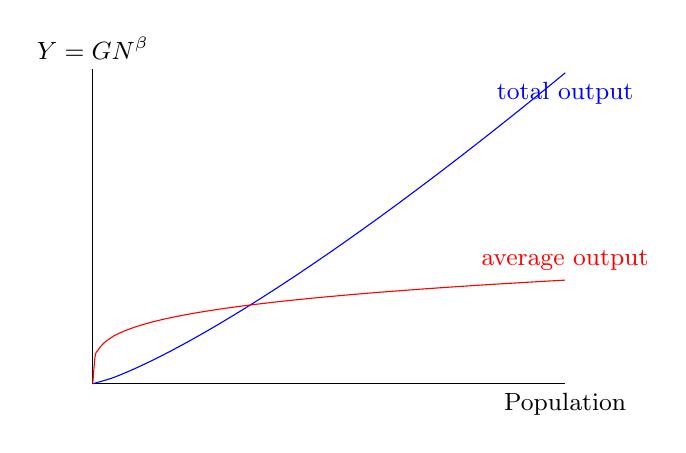
\begin{tikzpicture}
      \draw (0,4)node[above]{$Y= GN^{\beta}$}--(0,0) --(6,0)node[below]{Population};
       \draw[scale=1, domain=0:6, smooth, variable=\x, blue] plot ({\x}, {(\x/2)^1.25})node[below]{total output };% divide by 2 to get it on the plot
       %\draw (0,1)node[left]{$\alpha$}--(6,3.5)node[left]{$\alpha +\rho P$};
      \draw[scale=1, samples=200,domain=0:6, smooth, variable=\x, red] plot ({\x}, {(\x/2)^.25})node[above]{average output};% THis is the wage plot
           %   \draw[red] plot[samples=200, domain=-0:6] function {(\x/2)^.25};%node[above]{wage};
      %  \node [left] at (0,2){$w=\rho P$};
         % \draw [dashed](0,3)node[left]{$Y_i$}--(6,3);
    \end{tikzpicture}\vspace{.5cm}
    \caption{Urban productivity is proportional to population, $\beta=1.13$}
    \label{fig:scale_output}
    \end{center}
\end{figure}
 
 This figure illustrates a worry for me - the \textbf{average income} - {a proxy for the wage?) rises with $N$ but not more rapidly than transportation costs.
 
\subsubsection{Output and wage}
We need a combination of classical and neoclassical distribution theory.

City output is divided among the classes of society. Neoclassical theory suggests wages are allocated according to marginal product and classical theory suggests rents according to the pattern of ownership.

Equation one, in effect determines a wage, (Given the observed values for the scaling coefficients for total wages and labor, $bW < 1.15$ and $bL < 1$, )  although there are many possible distributional specifications and many possible labour market and firm structures. Bettencourt provides two  estimates,  1.11 and 1.35, for the scale factor for urban personal income in the Brazil and South Africa respectively.\footnote{A more recent  study supports the Bettancourt results for Chiin Wu W, Zhao H, Tan Q, Gao P. An Urban Scaling Estimation Method in a Heterogeneity Variance Perspective. Entropy (Basel). 2019 Mar 28;21(4):337. doi: 10.3390/e21040337. PMID: 33267051; PMCID: PMC7514821.} 

\subsubsection{Wage and city size}
The third determines the extent of the city. This comes form the Alonzo model discussed in chapter XXXXA. 

% PROBABLY REMOVE - FIGURE REPEATS
\begin{figure}
    \begin{center}
     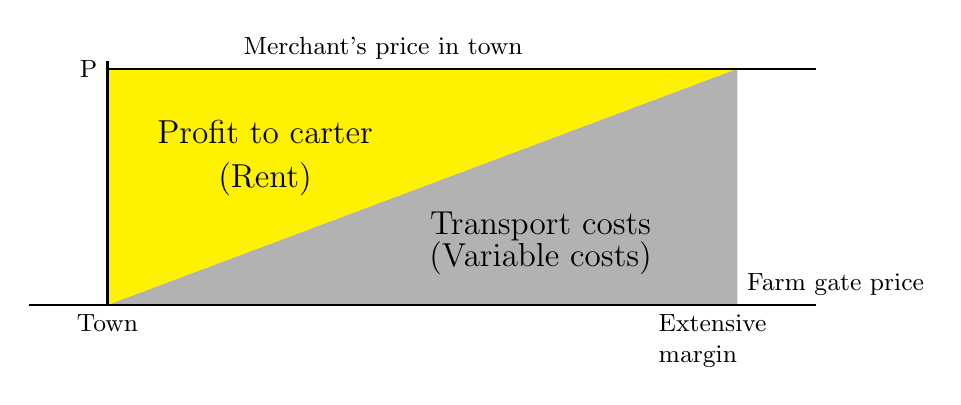
\begin{tikzpicture}[domain=0:2]
%\draw[thick,color=gray,step=.5cm, dashed] (-0.5,-.5) grid (3,3);
%\draw[line width=.01, green ] (0,0) -- (10,0) node[right  ] {Distance};
\node at (1,0) [below] {Town};
\fill[yellow]  (1,0) --(9,3)--(1,3) --cycle;
\fill[gray!60] (9,3) --(1,0)--(9,0) --cycle;

\draw[thick ] (1,3)node[left]{P}  -- (10,3);\node at (4.5,3)[above ] {Merchant's price in town} ;
\draw[thick ] (0,0)  -- (10,0); 

%\draw[thick,color=red] (1.5,0) -- (1.5,1) node[below right] {Fixed cost} -- (1.5,1.5) --(10,3.25)node[above left] {total cost};
\draw[thick] (1,0) -- (1,3.1) ;
\node[below,text width=2cm]at (9,0) {Extensive margin};
%\draw[ultra thick, blue,<-> ] (3,1.8) -- (3,2.5)node[left] {annual rent at a} -- (3,3) ; 
\node at (9,0)[above right] {Farm gate price};
\node  at (6.5,1){\large Transport costs};
\node  at (6.5,.6){\large (Variable costs)};
\node  at (3.,2.2){\large Profit to carter};
\node  at (3.,1.6){\large (Rent)};
\end{tikzpicture} 
    \caption{Transport costs, the yellow area, take a share of the profit for vegetables sold in the town}
    % \label{fig:rent_ricardo}
    \end{center}
\end{figure}

\begin{figure}
    \begin{center}
    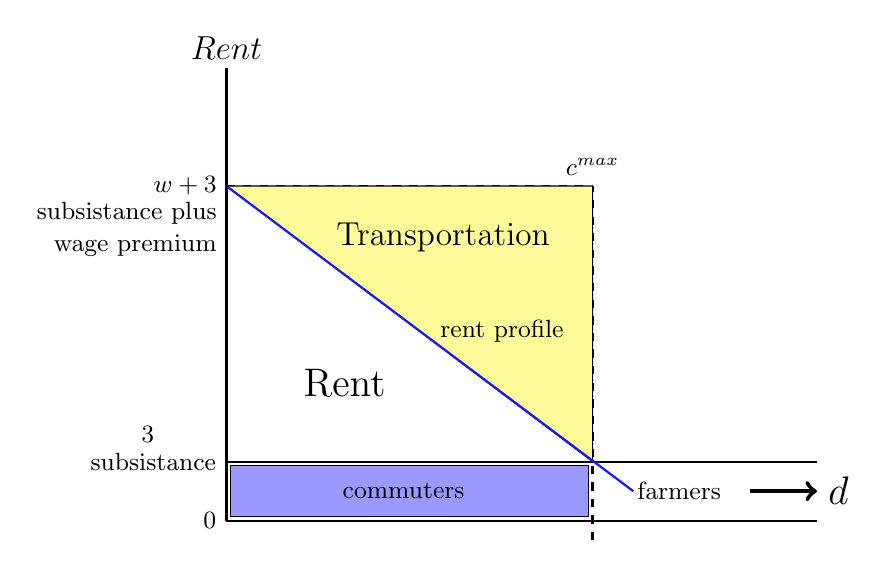
\begin{tikzpicture}[scale=.5]
\def\bndmax{5}        
\def\bndmin{0.2}
\def \n {10}  % height of y axis
\def \d {15}  % length  of x axis
\def \t {.75}  %  cost of transportation per unit x
\def \th {1}   %
\def \w {7}    %  wage premium
\def \om{1.5}%  omega =rural wage Zero for urban population
\def \azero{2}
\def \aprime {-.0}	
\tikzset{func/.style={thick,color=blue!90}}	
\draw [thick] (0,-\om) --(\d,-\om);  			% Zero for rural population
\draw [thick] (0,-\om)node[left]{$0$} --(0,\n);	% Y axis
\node at (0,\n+0.5){\large$Rent$};

\draw [thick] (0,0)node[left]{subsistance}--(\d,0);
\node a t(-2,.7) {$\omega$};
\node[left] at (0,\w){$w+\omega$};
\node[left] at (0,\w-.7){subsistance plus};
\node[left] at (0,\w-1.5){wage premium};	
\draw [dashed, thick](9.3,-2)-- (9.3,\w)node[above]{$c^{max}$};
\draw [dashed, thick](0,\w)-- (9.3,\w);
% solid color for commuters
\draw[fill=blue!40] (0.1,-0.1) rectangle (9.2,-\om+.1);
\draw[fill=yellow!40] (9.30,7.) -- (0,7)--(9.30,0.)--cycle;% Rent \w-.2
\draw[func,domain=0:\w/\t+1] plot [samples=200] (\x,{\w-\t*\x});
\node at (5.5,5.7){\large Transportation};
\node at (7,3.3){rent profile};		%Rent Profile	
\node at (3.,2){\Large Rent}; 		%Rent 
\node at (4.5,-\om/2){commuters};
\node at (11.5,-\om/2){farmers};
\draw [ ultra thick, ->](13.3,-\om/2)--(15, -\om/2)node [right] {\Large $d$};
\end{tikzpicture}
    \caption{A circular city with uniform transportation costs.}
    \label{fig:rent_alonzo}
    \end{center}
\end{figure}

A simple case is the circular city with uniform transportation cost, $t$. \[r^*= \frac{w}{t}\]% A more complex model might have density depend on location, for example, in the continous circular cityt\,
If transportation costs vary by  distance we might have something like this constraint on extent\[w=\int_0^{d*} t(d)dt.\]

This approach imposes an equilibrium condition on the model. It is unnecessary working with a citation of known extent and density. The analytic approach is easily extended to variable transportation cost, although at the expense of additional computational complexity.

\subsubsection{City extent and population}
Equation  four  closes the model by linking the extent of the city to the population. A simple case is the circular city with uniform population $d$, where $d$ is density per unit area and $r^*$ is the radius of the city: \[P=d\pi r^{*2}\] 
More generally, density might vary with for example, the distance $r$ from the centre of the city:
\[P=\pi \int_{0}^{r*}d(r)\,dr\] In a computational model a table of densities would provide the link.


\subsubsection{challenges}
maybe discuss some of the modeling challenges - division of income, lags, ???

\color{black}


\vspace{2cm}


\color{green}
 The growth of many cities was initially fueled by agricultural rents and resource exports. The industrial revolutions transformed many of these consumption cities into thriving production centers. 

while the ``origins'' of consumption cities can be traced to (i)
resource rents, (ii) rents from agricultural exports in countries with sufficiently high agricultural productivity, and (iii) ``premature'' deindustrialization.  Source:
%\href{https://www.brookings.edu/blog/future-development/2022/07/14/1622441/}
{Are cities engines of production or consumption, and does it matter?}








\subsection{Rent seeking}
  Rent-seeking is the act of growing one's existing wealth without creating new wealth by manipulating the social or political environment. Rent-seeking activities have negative effects on the rest of society. They result in reduced economic efficiency through misallocation of resources, reduced wealth creation, lost government revenue, heightened income inequality,


\color{black}
\chapter{Neoclassical Growth Theories} \label{chapter-growth}


The Cobb-Douglas form for representing production technology captured  important regularities in the cross-sectional national data,\footnote{ A 2021 meta-analysis of 3186 estimates concluded that "the weight of evidence accumulated in the empirical literature emphatically rejects the Cobb-Douglas specification."Gechert, Havranek, Irsova, Kolcunova (2021), "Measuring capital-labor substitution: The importance of method choices and publication bias", Review of Economic Dynamics, doi:10.1016/j.red.2021.05.003, S2CID 236400765. More sophisticated models  such as the CES and translog functions have been developed  since.} 
but the estimates soon showed a systematic bias with time series. Essentially the value of the $A$ seemed to rise over time. Something that was not captured in the initial model  contributed to productivity over time: 
 \[Y=A(t)K^\alpha L^\beta\]


 \section{The Solow-Swann growth model}
In 1956 Robert Solow\footnote{A Contribution to the Theory of Economic Growth,  Robert M. Solow, The Quarterly Journal of Economics, Vol. 70, No. 1 (Feb., 1956), pp. 65-94. Stable URL: http://www.jstor.org/stable/1884513} provided a possible explanation, opening the field for a further series of refinements in an enterprise that became known as ``growth theory.''
\footnote{Solow and his contemporary, Edward F. Denison in his 1961 monograph, \textit{The Sources of Economic Growth in the United States}, were attempting to account for the main features of U.S. economic growth, not to provide a theory of economic development.}%   R.E. Lucas, Jr., On the mechanics of economic development.}

Solow argued ``As a result of exogenous population growth the labor force increases at a constant relative rate n,'' so
  \[L(t)= L_0e^{nt}\] 
If we insert this term into the production function 
 \begin{eqnarray}
 Y&=cK^\alpha (L_0e^{nt})^\beta\\
    &=c(e^{nt})^{\beta}K^\alpha L^\beta\\
  %  &=A(t)K^\alpha L^{1-\alpha} \label{Eq:Solow}
 \end{eqnarray}
we see that $A$ becomes
 \[A(t)=c(e^{nt})^\beta\]
and we have a version of the time-dependent term needed to  allow the model to track the data better. More than half  of the cross-country variation in income can be explained by per capita saving and population growth alone.



%???       It is no surprise that adding a variable allowed the model to track the data better. More  interesting is that the appearance of term $1-\alpha}$ in the scale factor $A$ suggests a spillover effect of human capital on the productivity of other factors.\footnote{Breton, T. R. (2013). "Were Mankiw, Romer, and Weil Right? A Reconciliation of the Micro and Macro Effects of Schooling on Income" (PDF). Macroeconomic Dynamics. 17 (5): 1023–1054. doi:10.1017/S1365100511000824. hdl:10784/578. S2CID 154355849.}  

%The estimated model explained 78\% of the variation in income across countries.
% the estimates of $\beta$ implied that\textbf{ human capital's external effects on national income are greater than its direct effect on workers' salaries.}%(\url{https://en.wikipedia.org/wiki/Solow\%E2\%80\%93Swan_model)}.  Theodore Breton provided an insight that reconciled the large effect of human capital from schooling in the Mankiw, Romer, and Weil model with the smaller effect of schooling on workers' salaries. He demonstrated that the mathematical properties of the model include significant external effects between the factors of production because human capital and physical capital are multiplicative factors of production.[20] The external effect of human capital on the productivity of physical capital is evident in the marginal product of physical capital:
%    \[ MPK={\frac {\partial Y}{\partial K}}=\frac {\alpha A^{1-\alpha }(H/L)^{\beta }}{(K/L)^{1-\alpha} }\]


Solow's 1956 paper stimulated a vast literature in the 1960s, exploring many variations on the original one-sector structure. % (per Lucas on mechanics), See Burmeister and Dobell (1970) for an excellent introduction and survey. 
In these models, saving and population growth rates determine the growth trend of the economy. An important  contribution of the neoclassical framework stems from its ability to quantify the effects of various influences on growth. The estimated influences of saving and population growth with the Solow model appear too large, however.%Ludcas on the mechanics of ec dev
\footnote{In 1992, N. Gregory Mankiw, David Romer %(not to be confused with Paul M. Romer, mentioned above and below) 
and David N. Weil analyzed Solow’s Model in their paper “Contribution to the Empirics of Economic Growth” and  showed that %Solow correctly predicts the directions of saving and population growth, but not the orders of magnitude. Furthermore they pointed out that, 
if the model was augmented by including human capital $H$, it would fit the data even better.   (Mankiw et al. 1992). Their equation was, in our notation   \[Y=A(t)K^\alpha H^\gamma L^\beta\label{Eq:Mankiw}\] They assume $\alpha+\gamma<1$ which implies decreasing returns to all capital.} 
To understand the relation between saving, population growth, and income, it was necessary to go beyond the textbook Solow model.%, which assumed  diminishing returns to capital and labor separately and constant returns to both factors jointly, 


To understand the subsequent growth theories based on human capital, or what is sometimes called `effective labour' it is helpful to notice that Solo's formulation is unchanged if we substitute `labour times  skill' for $L$ in his model. both components of `labour times  skill,' or effective labour grow over time. The apparent effect of increasing labour supply could be, in fact, the combined effect of rising labour supply and increasing labour skill. Later studies would disentangle the two.

% MISSED Mankiw et al equation 
 % The  model became\footnote{Because they work with time series, all the quantities are dated. We omit the time marker for notational simplicity.}

In 1988, Robert E. Lucas would observe that ``It seems to be universally agreed that the model ... is not a theory of economic development.   \dots while it is not exactly wrong to describe these differences (in GDP  growth rates) by an exogenous, exponential term like A(t) neither is it useful to do so. We want a formalism that leads us to think about individual decisions to acquire knowledge, and about the consequences of these decisions for productivity.''\footnote{Lucas,  Robert E. On the Mechanics of Economic Development. Journal of Monetary Economics 22, 1988 3-42} 

% NOTE for  K   
%If we replace the labor-capital technology of the Solow model with a land-labor technology of the same form, and treat labor as the mobile factor and land as the immobile, we obtain a model that predicts exactly the immigration flows that occurred and for exactly the reason - factor price differentials - that motivated these historical flows



One of the predictions of the neoclassical growth model, even  when the concept of capital includes human capital, is that without  continuing improvements in technology, per capita income growth eventually ceases on the equilibrium path. 
By treating technological change as exogenous, neoclassical growth theory could not focus on the fundamental forces which determine long-run growth of nations. Theorists got around the problem to some extent by assuming that technological progress occurs in an exogenous manner. 

The models that followed, starting with Arrow's 1962 model of `learning by doing', introduce human capital and learning in a variety of ways. This is a central insight. Human capital may enter  as a stock that accumulates in the firm or the sector (Arrow (1962), Levhari (1966), and Sheshinski (1967b)) (proxied by aggregate prior capital investment.)
%(Levhari-Sheshinski)as  the experience of workers, the number of units previously produced, 
or the amount of innovation in other firms and sectors. % ( King and Robson )


Identifying  plausible ways that human capital might affect development was relatively easy. Measurement of human capital presents great practical difficulties. To extract the implications of a particular path, it was also necessary to construct a tractable model, analyze its dynamic properties, and find proxy data to test the initial hypothesis.   A series of papers did exactly that.

Kenneth Arrow (1962) gave a dynamic interpretation to increasing returns by emphasizing 'Learning by Doing'. This was an early attempt to render technological progress endogenous in growth models by making the productivity of a given firm an increasing function of cumulative aggregate investment for the industry. Productivity rises with cumulative firm output.


 It is important to note that these models all open the possibility that governments can  promote growth through investment in education, research, technology transfer, and incentives for firms.

\subsection{Endogenous (neoclassical) growth models}
A new wave of research on economic growth was stimulated by Romer (1986) and Lucas (1988). In their models, returns to scale are external to single economic agents and internal to a sector or larger parts of the economy. We apply the same insight to urban models to incorporate the growth-enhancing effect of agglomeration. 

%Basically, two branches have developed, pioneered by Romer (1990) and Lucas (1988). CHECK THESE SOURCES

Paul Romer's 1986  model\footnote{ based on his 1983 thesis} describes `learning by investment'. In this model, the increase in total factor productivity depends on firms’ learning, or investment in knowledge accumulation through research, rather than output. He models the incentives for the production of knowledge explicitly. The production function  can be written

\[Y = A(R^T)R^\gamma  K^\alpha L^\beta) \]
Where $R(\equiv R_i)$ is the research effort of the specific firm, and $R^T=\sum_iR_i$ is the total research in the industry,  $R$ is a choice variable for the firm, which is to say, it decides how much to invest in research. 

A notable feature of this model is the spillover effect on all other firms of the firm's investment through the Total Factor Productivity term,  $A(R^T)$. \textbf{This is the logic of our own model of agglomeration effects in the city.}



In 1988 Lucas also argued that technical progress is not exogenous, but endogenous. He proposed a model that is very close technically to the similar models of Arrow (1962), Uzawa (1965)and Romer (1986). Following our notation, 
\[ Y = A(H^e) K^\alpha (HeL)^\beta \] 
where $H^e$ is the economy's average level of skill (human capital).  Improvements in skill in any firm  increase overall productivity.  $HeL$  can be understood as the `effective' labour force of the firm. It is a product of $L$, size of the workforce. $H$, is the skill level of the firm's workers, and $e$, is the fraction of work time spent working. $1-e$ is the fraction of worker time  spent in training. The  special feature is that $e$ is a choice variable for the firm.\footnote{It could as easily be a choice variable for workers in the aggregate model.} More time training increase $H$ but reduces $e$, so the firm faces a tradeoff.


The difference between Romer and Lucas style theories is that endogenous growth in the theory of Romer is caused by accumulating technology (or knowledge), while in Lucas it is through training (accumulating human capital)\footnote{Although it is not of direct concern for our work, it is useful to recognize that much of the emphasis in these models is on finding the conditions that can explain the observed long term  and growth over and above that driven by exogenous population or technology growth. }

%THIS NEXT PARAGRAPH A SIMPLE COPY. FIND SOURCE

Again we see the  internal effects of human capital, where the individual worker undergoing training becomes more productive, and an external or `spillover' effect which increases the productivity of the economy. 
The evidence supports the existence of significant learning spillovers in a variety of industries. Using survey data, Mansfield (1985) found that information about new processes and products in ten industries surveyed had widely diffused within a year. Spillovers have also been found in econometric studies: Irwin and Klenow (1994) find them in semiconductors; Thornton and Thompson (2001) in wartime shipbuilding; Lieberman (1989) in chemicals; Foster and Rosenzweig (1995) in the adoption of high-yielding seed varieties; and Conley and Udry (2007) in the adoption of best practices by Ghanaian pineapple farmers. 

\subsection{Neoclassical production theory and the city}
%\href{https://www.yourarticlelibrary.com/economics/new-theory-of-growth-of-economic-development/38329}{New Theory of Growth of Economic Development}Supriya Guru

In all of these models, the unit of analysis is the nation,  or the firm. Lucas has suggested,\footnote{Journal of Monetary Economics 22 (1988) 3-42.  ON THE MECHANICS OF ECONOMIC DEVELOPMENT*
Robert E. LUCAS, Jr., University of Chicago, Chicago, 1L 60637, USA}
however, that `` a national economy is a completely arbitrary unit to consider.'' and that ``we know from ordinary experience that there are group interactions that are central to individual productivity and that involve groups larger than the immediate family and smaller than the human race as a whole.''  


As a result, ``following very closely the lead of Jane Jacobs, whose remarkable book The Economy of Cities (1969)'', Lucas goes on to suggest `` that the 'force' we need to postulate account for the central role of cities in economic life is of exactly the same character as the 'external human capital' I have postulated as a force to account for certain features of aggregative development.''  He concludes that if this is so, ``\textbf{\dots land rents should provide an indirect measure of this force (emphasis  ours)}, in much the same way that schooling-induced earnings differentials provide a measure of the productive effects of internal human capital. ''

This insight, which parallels ours, has not been adequately explored, in our view.  Allowing Lucas to expand on his observation about Jabobs, 


\begin{quotation}
    Her emphasis on the role of cities in economic growth stems from the observation that a city, economically, is like the nucleus of an atom: If we postulate only the usual list of economic forces, cities should fly apart. \textbf{The theory of production contains nothing to hold a city together.} (empahsis ours) A city is simply a collection of factors of production - capital, people, and land - and land is always far cheaper outside cities than inside. Why don't capital and people move outside, combining themselves with cheaper land and thereby increasing profits? Of course, people like to live near shopping and shops need to be located near their customers, but circular considerations of this kind explain only shopping centers, not cities. Cities are centered on wholesale trade and primary producers, and a theory that accounts for their existence has to explain why these producers are apparently choosing high rather than low-cost modes of operation.
\end{quotation}

This observation provides a natural link to the scaling literature on cities.


\section{Cities and the scaling literature}
Neoclassical production theory does not address the spatial structure of the economy. Why are there cities? What drives the historic transition from land-based agricultural society to a much denser urban society? 

In The Economy of Cities (1969) Jane Jacobs argued that when people come together in cities they make each other more productive. This is in essence, a theory of urban agglomeration that could be written
\begin{equation}\label{eq:LtoN}
Y = A(t) K(t)^\alpha L^\beta 
\end{equation}
where $L$ stands for the size of the urban labour force. Since urban labour force and population are closely correlated, the familiar model is  observationally equivalent to
\begin{equation}\label{eq:N2}
Y = A(t)N^{\alpha+\beta}
\end{equation}
\footnote{ To see why, let  $cN$ be labour employed by capital in firms, where $N$ represents the urban population and  assume a constant capital-labor ratio $1/d$. Replace $K$ with $dcN$
\[Y = A(t) (dcN)^\alpha (cN)^\beta) \]
But  $dc^\alpha$ and $c^\beta$  are simply  multiplicative constants that can be incorporated into the scale factor $A$, so  the function becomes 
\[Y = A(d, c,\alpha, \beta, t)N^{\alpha+\beta}\]
}

A model of a national economy that uses the number of urban dwellers would track as well using the number employed. As countries develop, cities account for an ever-increasing share of  national populations and an ever-increasing share of national income.  This is  even more likely when we recall that the principle insights coming out of neoclassical growth theory point to human capital and education as the mystery factor in growth and cities are where the most skilled workers concentrate and where the strongest educational institutions tend to be. The mysterious contribution to growth pursued in the previous sections might  actually be a consequence of urbanization.

We have conventional diminishing returns to scale  if we impose the standard neoclassical assumption, 
$\alpha +\beta <1 $.\footnote{
The required condition is that 
$Y(\delta K,\delta L< \delta Y(K,L)$. 
In the function that we use to illustrate the models, 
$Y(\delta K,\delta L)= \delta^{\alpha +\beta}Y < Y(K,L)$.} 
That leaves us with a question: what do we need for Equation~\ref{eq:N1} to represent Jacobs' observation?  

The answer lies in making the synergies that Jacobs point to explicit: we require $N$ to generate a spillover effect similar to those  identified in neoclassical growth theory. There are three obvious generic ways to introduce such a term: $N$ can augment $A$, $K$, or $L$, 

NEEDS ALIGNMENT
  
\[Y = A*N^\gamma K^\alpha N^\beta= AK^\alpha N^{\beta+\gamma}\]
\[Y = A (N^\gamma* K)^\alpha  N^\beta= AK^\alpha N^{\beta+\gamma^\alpha}\]
\[Y = A K^\alpha (N^\gamma* N)^\beta= AK^\alpha N^{\beta+\gamma}\]

Each of these yields a form of
\[Y = AN^\psi\]
where $\psi> \alpha +\beta$ and may be greater than one. 
The question now is whether we can find estimates of $\psi$.

The evidence we need comes from another field. Complex systems theory is concerned with identifying and characterizing common design elements that are observed across diverse natural, technological and social complex systems. It focuses on general principles  identified in complex systems across many fields such as biology, physiology, ecology, stock markets, multi-user online  networks, data systems, human settlements.and urban systems.

Scaling analysis is a tool developed in complex systems science to investigate how extensive properties of the system vary with a system's size.  or scale.  In urban science, there are now many studies of  the relationships between urban population size and  features like urban economic output,  area, growth, traffic congestion costs, and even social  indicators like crime and homicide rates. Our particular interest is in studies linking city population  and  economic output. 

The model used is familiar. Omitting subscripts for time, $t$ and city, $i$, \footnote{Bettancourt (2021) writes the model \[Y_i = Y_0(t)N_i(t)^\beta e^{\xi(t)}\]. }
\[Y = Y_0e^{n(t)}N^\beta\]
where $Y_0$ is an initial value. Notice that this looks exactly like the form that we saw in the 
Solow-Swan model with the transform from $K^\alpha L^\beta$ to $N$.  The interpretation is different because the model is used to estimate the parameter $\beta$ and $e^{n(t)}$ is described  as an error term of the form commonly used in estimating multiplicative time-series models. As a result estimates of $\beta$  can be used as estimates  of $\psi$.

\vspace{1cm}
\textbf{\Large COPY BOTTOM FIVE ROWS OF TABLE ON BETTANCOURT PAGE 67}  


\vspace{2cm}
The empirical scale factor is a feature of  a static urban system, but, as we have seen it is essentially a growth model. If the population rises, output must rise more than proportionately, but if the population responds to the share of output, the population should then rise. This is a 

Much of growth theory was concerned with identifying the dynamics of such systems and in particular with the implications for the growth of incomes. The growth models, however, were not spatial models, and therefore abstracted from land rents And distribution. They have nothing to say about the distribution of city product and the effect that distribution might have on growth.\footnote{Early models employ a macroeconomic savings function which usually has a fixed savings rate, with savings being reinvested in productive capital. } 

\vspace{2cm}

\section{Equilibrium city size  in terms of scale factor} 
At this point we can briefly describe how the discussion of this chapter relates to our overall modelling. There are four basic equations in the model. The first two link output and the wage to population. 


\subsubsection{population and output}
Equation one, following Bettencourt (p65) says that  urban productivity is proportional to population via a scale factor: 
\[Y\propto N^{\beta}\]  
\footnote{ In contemporary US cities productivity increases by about 11\% with each doubling of their population.  Urban Scaling and the Production Function for Cities Lobo J, Bettencourt LMA, Strumsky D, West GB (2013) PLOS ONE 8(3): e58407. https://doi.org/10.1371/journal.pone.0058407 },
and has both theoretical and empirical support. 

% \begin{tabular}{ll}
% $Y$ is &Aggregate urban output, or GDP \\
% %$\alpha$ & agricultural wage\\
% $G$ is&a `prefactor', possibly time dependent, an initial population\\
%  $N$ is& city population\\
% $ \beta$  is& scale factor, the elasticity of output with respect to city population .\\
% \end{tabular}\vspace{.5cm}

This is illustrated below for $\beta=1.13$.

\begin{figure}
    \begin{center}
    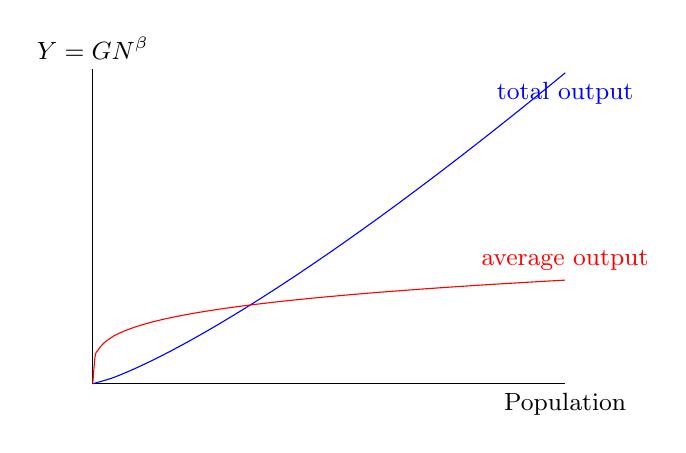
\begin{tikzpicture}
      \draw (0,4)node[above]{$Y= GN^{\beta}$}--(0,0) --(6,0)node[below]{Population};
       \draw[scale=1, domain=0:6, smooth, variable=\x, blue] plot ({\x}, {(\x/2)^1.25})node[below]{total output };% divide by 2 to get it on the plot
       %\draw (0,1)node[left]{$\alpha$}--(6,3.5)node[left]{$\alpha +\rho P$};
      \draw[scale=1, samples=200,domain=0:6, smooth, variable=\x, red] plot ({\x}, {(\x/2)^.25})node[above]{average output};% THis is the wage plot
           %   \draw[red] plot[samples=200, domain=-0:6] function {(\x/2)^.25};%node[above]{wage};
      %  \node [left] at (0,2){$w=\rho P$};
         % \draw [dashed](0,3)node[left]{$Y_i$}--(6,3);
    \end{tikzpicture}\vspace{.5cm}
    \caption{Urban productivity is proportional to population, $\beta=1.13$}
    \label{fig:scale_output}
    \end{center}
\end{figure}
 
 This figure illustrates a worry for me - the \textbf{average income} - {a proxy for the wage?) rises with $N$ but not more rapidly than transportation costs.
 
\subsubsection{Output and wage}
We need a combination of classical and neoclassical distribution theory.

City output is divided among the classes of society. Neoclassical theory suggests wages are allocated according to marginal product and classical theory suggests rents according to the pattern of ownership.

Equation one, in effect determines a wage, (Given the observed values for the scaling coefficients for total wages and labor, $bW < 1.15$ and $bL < 1$, )  although there are many possible distributional specifications and many possible labour market and firm structures. Bettencourt provides two  estimates,  1.11 and 1.35, for the scale factor for urban personal income in the Brazil and South Africa respectively.\footnote{A more recent  study supports the Bettancourt results for Chiin Wu W, Zhao H, Tan Q, Gao P. An Urban Scaling Estimation Method in a Heterogeneity Variance Perspective. Entropy (Basel). 2019 Mar 28;21(4):337. doi: 10.3390/e21040337. PMID: 33267051; PMCID: PMC7514821.} 

\subsubsection{Wage and city size}
The third determines the extent of the city. This comes form the Alonzo model discussed in chapter XXXXA. 

% PROBABLY REMOVE - FIGURE REPEATS
\begin{figure}
    \begin{center}
     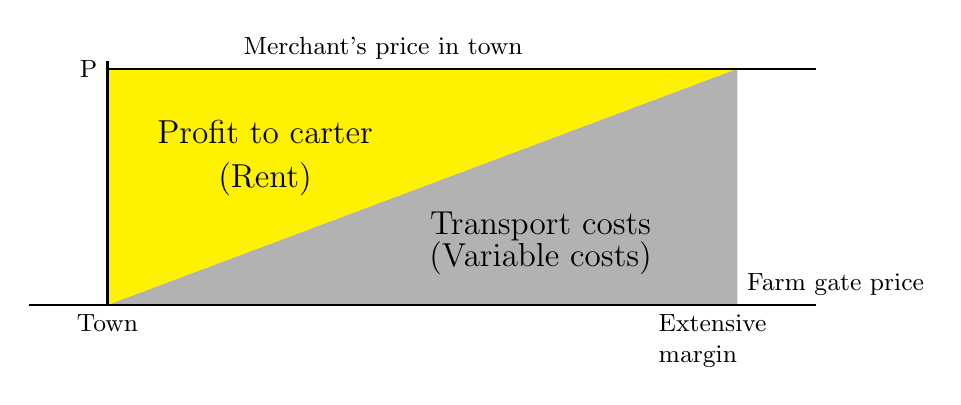
\begin{tikzpicture}[domain=0:2]
%\draw[thick,color=gray,step=.5cm, dashed] (-0.5,-.5) grid (3,3);
%\draw[line width=.01, green ] (0,0) -- (10,0) node[right  ] {Distance};
\node at (1,0) [below] {Town};
\fill[yellow]  (1,0) --(9,3)--(1,3) --cycle;
\fill[gray!60] (9,3) --(1,0)--(9,0) --cycle;

\draw[thick ] (1,3)node[left]{P}  -- (10,3);\node at (4.5,3)[above ] {Merchant's price in town} ;
\draw[thick ] (0,0)  -- (10,0); 

%\draw[thick,color=red] (1.5,0) -- (1.5,1) node[below right] {Fixed cost} -- (1.5,1.5) --(10,3.25)node[above left] {total cost};
\draw[thick] (1,0) -- (1,3.1) ;
\node[below,text width=2cm]at (9,0) {Extensive margin};
%\draw[ultra thick, blue,<-> ] (3,1.8) -- (3,2.5)node[left] {annual rent at a} -- (3,3) ; 
\node at (9,0)[above right] {Farm gate price};
\node  at (6.5,1){\large Transport costs};
\node  at (6.5,.6){\large (Variable costs)};
\node  at (3.,2.2){\large Profit to carter};
\node  at (3.,1.6){\large (Rent)};
\end{tikzpicture} 
    \caption{Transport costs, the yellow area, take a share of the profit for vegetables sold in the town}
    % \label{fig:rent_ricardo}
    \end{center}
\end{figure}

\begin{figure}
    \begin{center}
    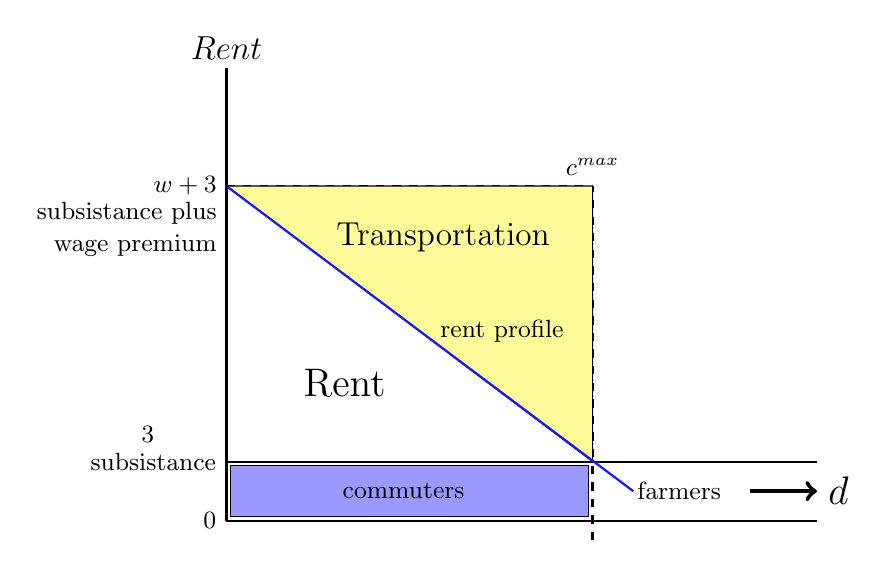
\begin{tikzpicture}[scale=.5]
\def\bndmax{5}        
\def\bndmin{0.2}
\def \n {10}  % height of y axis
\def \d {15}  % length  of x axis
\def \t {.75}  %  cost of transportation per unit x
\def \th {1}   %
\def \w {7}    %  wage premium
\def \om{1.5}%  omega =rural wage Zero for urban population
\def \azero{2}
\def \aprime {-.0}	
\tikzset{func/.style={thick,color=blue!90}}	
\draw [thick] (0,-\om) --(\d,-\om);  			% Zero for rural population
\draw [thick] (0,-\om)node[left]{$0$} --(0,\n);	% Y axis
\node at (0,\n+0.5){\large$Rent$};

\draw [thick] (0,0)node[left]{subsistance}--(\d,0);
\node a t(-2,.7) {$\omega$};
\node[left] at (0,\w){$w+\omega$};
\node[left] at (0,\w-.7){subsistance plus};
\node[left] at (0,\w-1.5){wage premium};	
\draw [dashed, thick](9.3,-2)-- (9.3,\w)node[above]{$c^{max}$};
\draw [dashed, thick](0,\w)-- (9.3,\w);
% solid color for commuters
\draw[fill=blue!40] (0.1,-0.1) rectangle (9.2,-\om+.1);
\draw[fill=yellow!40] (9.30,7.) -- (0,7)--(9.30,0.)--cycle;% Rent \w-.2
\draw[func,domain=0:\w/\t+1] plot [samples=200] (\x,{\w-\t*\x});
\node at (5.5,5.7){\large Transportation};
\node at (7,3.3){rent profile};		%Rent Profile	
\node at (3.,2){\Large Rent}; 		%Rent 
\node at (4.5,-\om/2){commuters};
\node at (11.5,-\om/2){farmers};
\draw [ ultra thick, ->](13.3,-\om/2)--(15, -\om/2)node [right] {\Large $d$};
\end{tikzpicture}
    \caption{A circular city with uniform transportation costs.}
    \label{fig:rent_alonzo}
    \end{center}
\end{figure}

A simple case is the circular city with uniform transportation cost, $t$. \[r^*= \frac{w}{t}\]% A more complex model might have density depend on location, for example, in the continous circular cityt\,
If transportation costs vary by  distance we might have something like this constraint on extent\[w=\int_0^{d*} t(d)dt.\]

This approach imposes an equilibrium condition on the model. It is unnecessary working with a citation of known extent and density. The analytic approach is easily extended to variable transportation cost, although at the expense of additional computational complexity.

\subsubsection{City extent and population}
Equation  four  closes the model by linking the extent of the city to the population. A simple case is the circular city with uniform population $d$, where $d$ is density per unit area and $r^*$ is the radius of the city: \[P=d\pi r^{*2}\] 
More generally, density might vary with for example, the distance $r$ from the centre of the city:
\[P=\pi \int_{0}^{r*}d(r)\,dr\] In a computational model a table of densities would provide the link.


\subsubsection{challenges}
maybe discuss some of the modeling challenges - division of income, lags, ???

\color{black}


\vspace{2cm}


\color{green}
 The growth of many cities was initially fueled by agricultural rents and resource exports. The industrial revolutions transformed many of these consumption cities into thriving production centers. 

while the ``origins'' of consumption cities can be traced to (i)
resource rents, (ii) rents from agricultural exports in countries with sufficiently high agricultural productivity, and (iii) ``premature'' deindustrialization.  Source:
%\href{https://www.brookings.edu/blog/future-development/2022/07/14/1622441/}
{Are cities engines of production or consumption, and does it matter?}




\subsection{Rent seeking}
  Rent-seeking is the act of growing one's existing wealth without creating new wealth by manipulating the social or political environment. Rent-seeking activities have negative effects on the rest of society. They result in reduced economic efficiency through misallocation of resources, reduced wealth creation, lost government revenue, heightened income inequality,


\color{black}
\chapter{Urban Land and Land Rent} \label{chapter-space}

\section{The Alonzo-Jacobs model}
In 1964, William Alonso published \textbf{Location and Land Use}, in which he described a model that specifically linked the urban wage premium to urban land rents and  became the central model in modern urban economics. 
We use an \textbf{Alonzo-Jacobs model} to explore the source and distribution surplus value, where the reference to Jane Jacobs links the wage premium to Jacobs-style  agglomeration effects that generate urban productivity.% and the wage premium. 

Ricardo had described a model with a central market for corn, producing corn took land and transporting corn to market was costly. Because there is one market price for corn, land with low transportation costs near the central market earns a rent. More distant land has lower value. In Alonzo's model there is central market and a single price for labour, producing labour takes land, and transporting labour to the market is costly. Alonzo simply re-presents Ricardo's conception of rent  mathematically for a different social system and production technology.  

The logic of the model is illustrated in the following figure. The height of the green bar on the left illustrates the premium for urban labour at the centre of an Alonzo circular city. The height red triangle at the left is the rent earned on land at the centre, which has no transportation costs.\footnote{The model says nothing about who gets the rent in the urban economy. For classical economists it was obvious that the agricultural rents went to the class of land-owners.} Transportation to and from the center costs $t$ times the distance $d$ from the center. Fuel, capital, and time costs are  all included in $t$. 


\begin{figure}
    \begin{center}
    
% Simple Alonzo model
%%%%%%%%%%%%%%%%%%%%%%%% PARTITIONING THE LABOUR SHARE
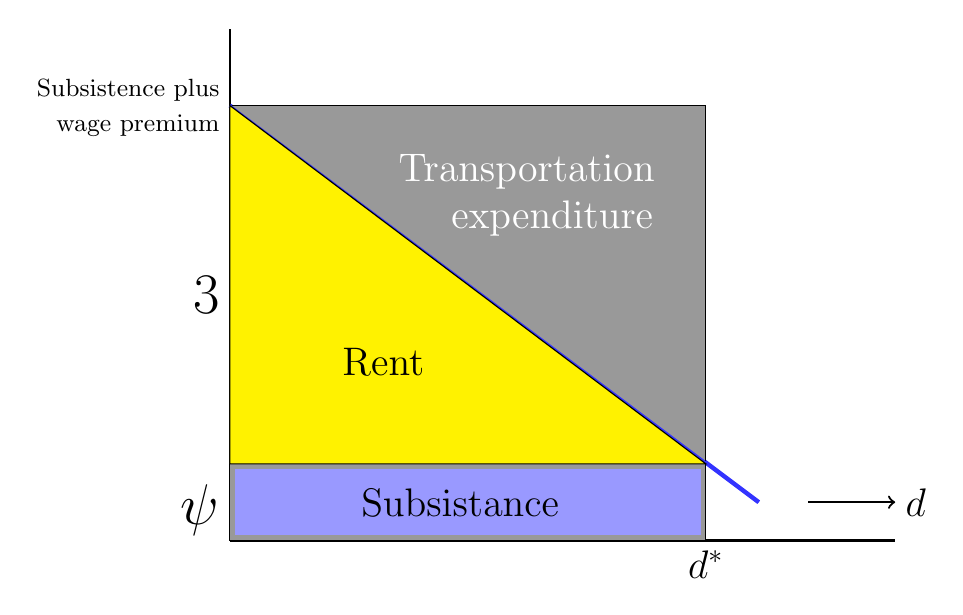
\begin{tikzpicture}[scale=.65]
\def\bndmax{5}        %https://tex.stackexchange.com/questions/68462/filling-a-complex-region-with-tikz
\def\bndmin{0.2}
\def \n {8.5}  % height of y axis
\def \d {13}  % length  of x axis
\def \t {.75}  %  cost of transportation per unit x
\def \th {1}   %
\def \w {7}    %  wage premium
\def \om{1.5}%  omega =rural wage Zero for urban population
\def \azero{2}
\def \aprime {-.0}	
\tikzset{func/.style={thick,color=blue!80}}	

% FIRST FIGURE just axes PARTITIONING THE LABOUR SHARE
\draw [thick] (0,-\om) --(\d,-\om);  			% Zero for rural population
\draw [thick] (0,-\om) --(0,\n); %node[above]{\Huge $w$};	% Y axis
%\node at (0,\n+0.5){\large $Rent$};

% \draw [thick] (0,0)node[left=.5]{Subsistence}--(\d,0);
%\node at(-2,1) {$\omega$};
\node[left=.25] at (0,3.3){\huge $\omega$};
\node[left=.25] at (0,-0.9){\huge $\psi$};
%\node[left=.25] at (0,3){$w+\omega$};
\node[left=.25] at (0,\w+.3){Subsistence plus};
\node[left=.25] at (0,\w-.4){wage premium};	

%\foreach \xi in {0,..., \n} \draw (\xi,0)--(\xi,-.1)node[below=1]{\small$\xi$};
%\foreach \yi in {1,...,\n} \draw (0,\yi)--(-.1,\yi)node[left]{$\yi$};
%\foreach \i in {1,4,9,16} {
%\node at (7,-\om/2){people scattered uniformly across the land  };

%SECOND FIGURE WITH AGGLOMERATION WAGE
%   \pause %  add urban production and net wage PARTITIONING THE LABOUR SHARE
%\draw[fill=white, white] (0.1,-0.1) rectangle (14,-\om+.1);
%\draw [fill=green!80] (-.25, 0) rectangle(.25, \w);
\node[right] at  (.25, \w/2){Added Productivity};
% \node[right, text width = 3cm] at  (10,9){Where does the increase in productivity come from?};
\draw [ thick, ->](11.3,-\om/2)--(13, -\om/2)node [right] {\Large $d$};

%  THIRD FIGURE  add wage profile PARTITIONING THE LABOUR SHARE
% \pause
%\node[right, white, fill=white,  text width = 3cm] at  (10,9){Where does the increase in productivity come from?};
\draw[func, domain=0:\w/\t+1,ultra thick] plot [samples=200] (\x,{\w-\t*\x}); %Net wageprofile  for 
%\node[right, white, fill=white] at  (.25, \w/2){Added Productivity};
%\node[right, fill=white, text width =3.5cm ] at  (1, \w/2){Declining wage  net \\of transportation\\ costs $T(d)$ };

%   FOURTH FIGURE     commuters PARTITIONING THE LABOUR SHARE
%\pause
%\draw[fill=blue!40] (0.1,-0.1) rectangle (9.2,-\om+.1);
%\node at (4.5,-\om/2){commuters};

%   FOURTH FIGURE    wage bill
%\pause %add total new value
\draw[fill=green!40] (0,-\om) rectangle(9.30,\w);% new product
\node at (4.5,\w/2){\Large urban wage bill};

%%   FIFTH FIGURE   distribution
%\pause
%\node at (9,\n){\Large Partitioning the Labour Share};

\draw[fill=black!40] (0,-\om) rectangle (9.30,\w);% new product repeat
\draw[func, domain=0:\w/\t+1] plot [samples=200] (\x,{\w-\t*\x}); %rent profile
\fill[blue!40] (0.1,-0.1) rectangle (9.2,-\om+.1);
\node at (4.5,-\om/2){\Large Subsistance};
\draw[fill=yellow,] (0.,0.) -- (0,7)--(9.30,0.)--cycle;% Rent \w-.2
\node at (3.,2){\Large Rent}; 		%Rent 
\node at (5.8,5.7)[white]{\Large Transportation};
\node at (6.3,4.8)[white]{\Large expenditure};
\node at (9.3,-1.5)[below]{\Large  $d^*$};
% \node at (4.8,\w)[above]{\huge $d^*$};
 \end{tikzpicture}
 

    \caption{}
    \label{fig:city_simple_alonzo}
    \end{center}
\end{figure}


% %%%%%%%%%%%%%%%%%%%%%%%% PARTITIONING THE LABOUR SHARE
The entire rectangle, $\omega$ $\times$ $d^*$, is the surplus generated by urban agglomeration. Urban land rent, which is the residual when transport costs are deducted from the wage premium, declines  with distance $d$ until, at the very edge of the city, $d^*$, t the cost of transportation  consumes the entire wage. Property values are simply the the present discounted value of the rent at any point.

At the bottom of the figure we illustrate the conventional `subsistence wage'  earned by a worker whether in the city or outside of the city.   In most analyses of urban spaces this living wage is simply ignored, since it is the wage premium that generates rents.  It is also common to assume that the labour market and production at the centre takes no space.   


Workers are attracted to the city by the wage premium, $\omega$,  which represents the share of the surplus generated by the city that goes to labour.  The grey triangle represents the amount of the surplus dissipated in travel costs.  

The extent  of the city  $d^*$ is a simply the distance at which total $rt$ transportation cost  is equal to the wage premium
\[d^* t= \omega\]
where $t$ is the unit cost of transportation. In the figure, $-t$ is the slope of the diagonal line dividing rent from transportation expenditure.



 \section{Implications and results from Alonzo's circular city}
 It is a beautifully simple model that accounts for many features of urban structure and urban history. In this section we describe some of the insights supported by the model. Extensions can incorporate variation in wages, density, transportation costs,  preference, and even building technology and codes. The limitations of the simple, continuous, equilibrium based versions described above can be overcome using agent-based models to model the evolution of complex and much more realistic urban systems. 

 \subsection{The magnitude of rents and transportation costs}
 From $w$, $t$ and population density we can derive population, wage bill, total rent, transportation costs. The figure above suggest that  half of the urban surplus is spent on transportation, but because the city is circular, the total value of rents can be represented as the volume  \[ V=\frac{1}{3}\pi  d^{*2} \omega \]
of a cone with radius $d^*$ and  height $\omega = td^*$. Substituting out either  $\omega$ or  $d^*$, we find that total rent is  proportional to the \textbf{cube} of either  $d^*$ or $\omega$. 

The total value of wage payments would appear as the volume of cylinder enclosing the cone\footnote{since the wage is the same for each unit of labour no matter where is t is produced (resides).}.  
$V=\pi r^2 \omega$


 \vspace{1cm}

\begin{figure}
    \begin{center}
    
\begin{tikzpicture}[scale=.5]
   %%%%%%%%%%%%%%%%%%%%%%%%%%%%%%%%%%%%%%%%%%%%%%%%
% definitions for schematic
\def\bndmax{5}        %https://tex.stackexchange.com/questions/68462/filling-a-complex-region-with-tikz
\def\bndmin{0.2}
\def \n {10}  % height of y axis
\def \d {12}  % length  of x axis
\def \t {.75}  %  cost of transportation per unit x
\def \th {1}   % theta?
\def \w {7}    %  wage premium
\def \om{1.5}%  omega =rural wage Zero for urban population
\def \azero{2}
\def \aprime {-.0}	
\tikzset{func/.style={thick,color=blue!90}}	

    %%%%%%%%%%%%%%%%%%%%%%%%%%%%%%%%%%%%%%%%%%%%%%%%
% definitions for Cone3
%\node at (0, 2.5){\input{SA_Cone3.tex}};
     \pgfmathsetmacro{\radiush}{9.7};%Cone base radius was 9.6
        \pgfmathsetmacro{\theight}{7.1}%Cone height (negative if you want a inverse cone)
        \pgfmathsetmacro{\cheightp}{.03}%Cut height in percent of cone height

        %Calculating coordinates
        \coordinate (center) at (0,0);
        \pgfmathsetmacro{\radiusv}{.2 * \radiush}; %HORIZONTAL RADIUS
        \coordinate (peak) at ($(center) + (0,\theight)$);     
        \pgfmathsetmacro{\sradiush}{\radiush * (1 - \cheightp)};%ADJUST FOR COVERAGE AT CORNERS
        \pgfmathsetmacro{\sradiusv}{.2 * \sradiush};
   %     \pgfmathsetmacro{\sradiusv} {\sradiusv -.1 };

\coordinate (antipeak) at ($(center) + (0,-\theight)$);  %thanks  %I added this
\coordinate (vert1) at ($(center)+(\radiush,-.2)$);
\coordinate (vert2) at ($(center)-(\radiush,.2)$);
%problem
   
\coordinate (svert1) at ($(vert1)!\cheightp!(peak) +(0.1,.75)$);
\coordinate (svert2) at ($(vert2)!\cheightp!(peak)+(.5,.75)$);  
    % \coordinate (svert3) at ($svert1+(0,\w)$);
    % \coordinate (svert4) at ($vert2)+(0,\w)$);  
    %  \coordinate (svert3) at ($svert1+(0,7)$ );  % Shifting up by W
    % \coordinate (svert4) at ($svert2 + (0,\w)$0;
   %%%%%%%%%%%%%%%%%%%%%%%%%%%%%%%%%%%%%%%%%%%%%%%%


 
%\draw[step=.5,black,thin] (-9.6,0) grid (9.6,7);
 
% Cone Drawing    
 \fill[ left color=red!70, right color=red!70,  opacity=20,middle color=red!20,shading=axis] (svert1) -- (peak) -- (svert2) arc (170:370:\sradiush cm and \sradiusv cm);

    % FAT GREEN BAR
 \draw [fill=green,opacity=80] (-.2, 0) rectangle(.2, \w);
 \node[above] at (0,\w){$\omega$};
 
%Uncomment this for top of cylinder
      \fill[inner color=gray!2,outer color=gray!40,shading=radial,opacity=.5] ($(center) + (.35,\theight)$ ) circle (9.4 cm and 1.55 cm );
      
        % \draw [thick]($(svert1) +(.3,-.3)$)-- ++ (90:\w-.2);
        % \draw [thick]($(svert2)-(.2,.3)$)-- ++ (90:\w-.2);
        %Lines, \h in percent of cone height
 def \sradiusv2 \sradiusv cm -.1 cm)
% Cylinder drawing
  \fill[ left color=black!50, right color=red!30,  middle color=red!30,shading=axis,opacity=.2]  (-9.05,.5) 
  arc (180:360:\sradiush cm and \sradiusv cm)-- ++(90:\w-.2) 
  arc (360:180:\sradiush cm and \sradiusv2 cm -.1 cm)--(-9.05,.5);  

   \node[above] at (0,\w){\Large $\omega$};
% TRY TO Make a cylinder
%\draw ($svert2 + (0,\theight)$) [arc (180:360:\sradiush cm and \sradiusv cm)]; 
%     \fill[left color=gray!70,right color=gray!70,middle color=gray!30,shading=axis] (vert1) -- (svert1) arc (0:-180:\sradiush cm and \sradiusv cm) -- (vert2) arc (180:360:\radiush cm and \radiusv cm);

% DASHED LINE AT BACK OF CONE
\foreach \h in {0.03}{   %.38,.34,.30, .7
            \pgfmathsetmacro{\rh}{-\radiush * (1 - \h)}
            \pgfmathsetmacro{\rv}{.2 * \rh}
            \draw[black!70,densely dashed] ($(svert2)!\h!(peak)-(.3,.9)$) arc (370:170:\rh cm and \rv cm);%$(vert2)!\h!(peak)$)
        }
  %      \draw[opacity=.90, line width=.05cm, green] (0,0)--(0,{\theight - .05});
%     \foreach \h in {0, .38,.34,.30, .7}{
%            \pgfmathsetmacro{\rh}{\radiush * (1 - \h)} %            \pgfmathsetmacro{\rv}{.2 * \rh}
%            \draw[black!70,densely dashed] ($(antipeak)!\h!(vert2)$) arc (180:360:\rh cm and \rv cm);
%   }
%  \draw[red] (antipeak) arc (30:60:3);
%  \draw[dashed, thick] arc (0:-180:\sradiush cm and \sradiusv cm) -- (vert2) arc (180:360:\radiush cm and \radiusv cm);
%%%%%%%%%%%%%%%%%%%%%%%%%%%%%%%%%

% %\foreach \xi in {0,..., \n} \draw (\xi,0)--(\xi,-.1)node[below=1]{\small$\xi$};
% %\foreach \yi in {1,...,\n} \draw (0,\yi)--(-.1,\yi)node[left]{$\yi$};
% %\foreach \i in {1,4,9,16} {
% %\node at (7,-\om/2){people scattered uniformly across the land  };

% %SECOND FIGURE WITH AGGLOMERATION WAGE
% %  add urban production and net wage
% %\draw[fill=white, white] (0.1,-0.1) rectangle (14,-\om+.1);

% \node[right, text width=4cm] at  (3, \w+1){Added Productivity due to agglomeration};
% %\node[right, text width = 3cm] at  (10,9){Where does the increase in productivity come from?};
 \draw [ thick, ->](0,0)--(2.5, 0)node [right] {\Large $d$};


% \draw[thick] (0,0) -- ++ (50:2.6cm);  %   diagonal for perspective
% \draw[thick] (0,0) -- ++ (230:2.35cm); 

% %  THIRD FIGURE  add RENT profile in blue

% %\node[right, white, fill=white,  text width = 3cm] at  (10,9){Where does the increase in productivity come from?};
% \draw[func, domain=0:\w/\t+1,ultra thick] plot [samples=200] (\x,{\w-\t*\x}); %Net wageprofile  for 
% %\node[right, white, fill=white] at  (.25, \w/2){Added Productivity};
% %\node[right, fill=white, text width =3.5cm ] at  (1, \w/2){Declining wage  net \\of transportation\\ costs $T(d)$ };
% %\node[right, fill=white, text width =3.5cm ] at  (4,9){Declining wage  net \\of transportation\\ costs  };
% %
% %\node at (0, 1.5){\includegraphics{\input{SA_Cone3.tex}} };
% %\node at (0, 2.5){\input{SA_Cone3.tex}};

% %   FOURTH FIGURE     commuters
% %\pause
% %\draw[fill=blue!40] (0.1,-0.1) rectangle (9.2,-\om+.1);
% \node at (4.5,.4*\om){commuters};


\end{tikzpicture}
    \caption{}
    \label{fig:city_conical}
    \end{center}
\end{figure}




 \vspace{1cm}
and total transport costs are 
$\frac{2}{3}\pi  d^{*2} \omega).$
With uniform density, population is proportional to the square of  $d^{*2}$ while rents and  transportation costs are proportional to the cube. 

\subsection {Changing transportation costs}

Another application of the model is to the effect of a transportation revolutution. Urbanists agree that before the railroad and the automobile the extent of a city was roughly determined by how far a person could walk in about an hour. The time and effort cost of transportation determined the size of cities. The advent of first rail transportation and then the automobile radically changed the size, productivity, and population distribution of cities

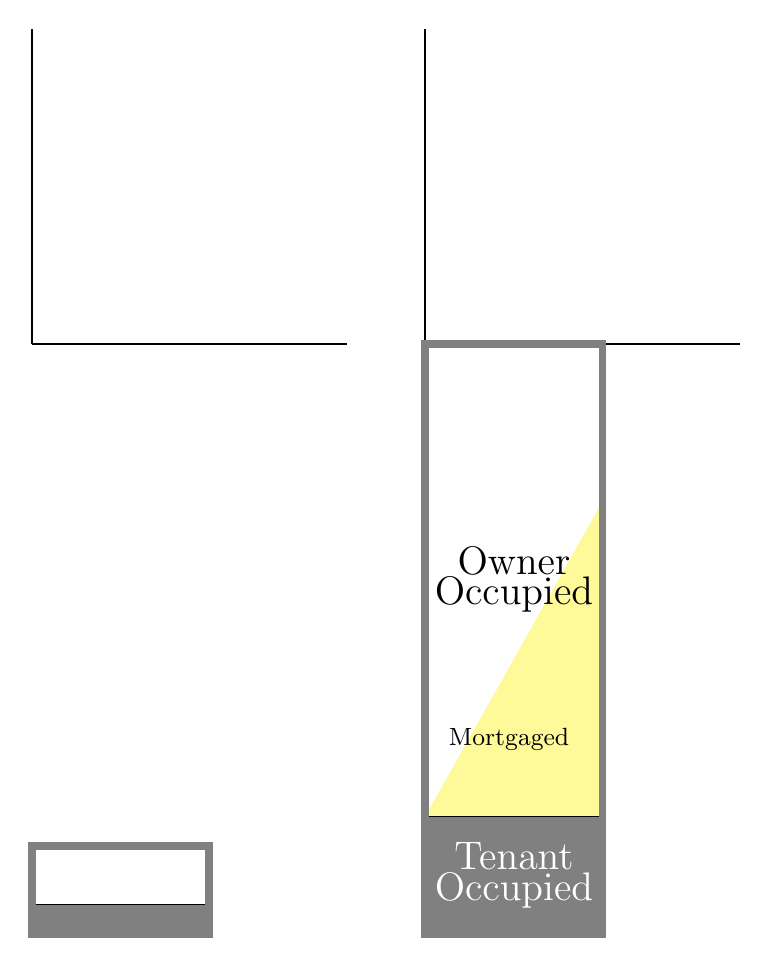
\begin{tikzpicture}[scale=.5]
\draw[thick](0,0)--(0,8);
\draw[thick](0,0)--(8,0);

\begin{scope}[shift={(0, -15cm)},scale=1.5]%population
\draw [fill=gray,] (0,0) rectangle (3,.5); %TENANT
\draw[line width= 1mm, black!50] (0,0) rectangle (3,1.5);
\end{scope}
\begin{scope}[shift={(10cm, 0)}]
\draw[thick](0,0)--(0,8);
\draw[thick](0,0)--(8,0);
\end{scope}

\begin{scope}[shift={(10, -15cm)},scale=1.5]%population
\draw [fill=gray,] (0,0) rectangle (3,2); %TENANT
\draw [fill=yellow!40] (0,2)--(3,2)--(3,7.33); --cycle;% 
\draw[line width= 1mm, black!50] (0,0) rectangle (3,10);
\node at (1.5,6)
    [text width=2.4cm, align=center]
    {\baselineskip=20pt\Large Owner Occupied};
\node at (2,3.3)
    [text width=2.4cm]
    {\baselineskip=20pt Mortgaged};
\node at (1.5,1)
    [text width=2.4cm, align=center, white]
    {\baselineskip=20pt\Large Tenant Occupied};
\end{scope}
 \end{tikzpicture}
 

It is easy to see that the transportation cost revolution brought about by first street cars and later automobiles made much larger cities possible.  The average walking pace is 2.5 to 4 mph, and new transportation technologies raises this rate by a factor of between five and ten, increasing potential urban area by between twenty-five and  one hundred times. 

It  also affected social structure and left indelible marks of the form of cities developing at the time and after.In North America, with large amounts of land, it generated massive urban sprawl, but also made land available for a growing `middle class.' Ultimately it generated congestion and rising transportation cost that began to limit urban growth. 

\section{Adding Jacobs-style agglomeration effects}
Belderbos, Ikeuchi and  \cite{} examine the simultaneous effects of spillovers due to R\&D by universities and by firms 
Rising urban productivity in Japan are significant. 

will raise the wage, attracting more workers. If they are added in suburbs at the edge of the city (Ricardo's extensive margin) virtually all of the wage premium they receive is dissipated in transportation costs. Closer to the centre,  land rents rise. Owner-occupiers capture the increase as property value appreciation. Tenants are likely to be faced with higher rents.      

If agglomeration is the source of productivity gains, however, the new workers increase the urban premium, further increasing land values and attracting more workers. 



The rural population consists of uniformly distributed efficient mix of rural capital producers and workers, all of whom receive $\omega$.%\footnote{This does nothing but fix the price of produced capital in terms of the rural wage.} 



 Owners of urban firms are  conventional  capitalists, who may earn excess profit if they can capture an unearned surplus from labour.  Any unearned surplus increases the return to urban capital relative to rural capital, resulting in continuous expansion of the urban economy. Continuous growth in turn results in continuously rising urban land prices and hence housing costs. We ignore the distributional implications of this feature of the model, and focus instead on the part of value produced by the city that appears as land rent. 
  
\section{Net land rent} 
The simple graphical model we consider above is revealing, but it leaves out many important features of the urban system. The only costs included are the transportation costs for the individual.  Since urban services and  a substantial fraction of urban amenities are financed through the public sector a more complete model must include both servicing costs and property taxation. The relevant rent profile from an economic point of view is NET of all service costs. From a finance point of view it is net of tax liabilities.

%%%%%%%%%%%%%%%%%%%%%%%% PARTITIONING THE LABOUR SHARE
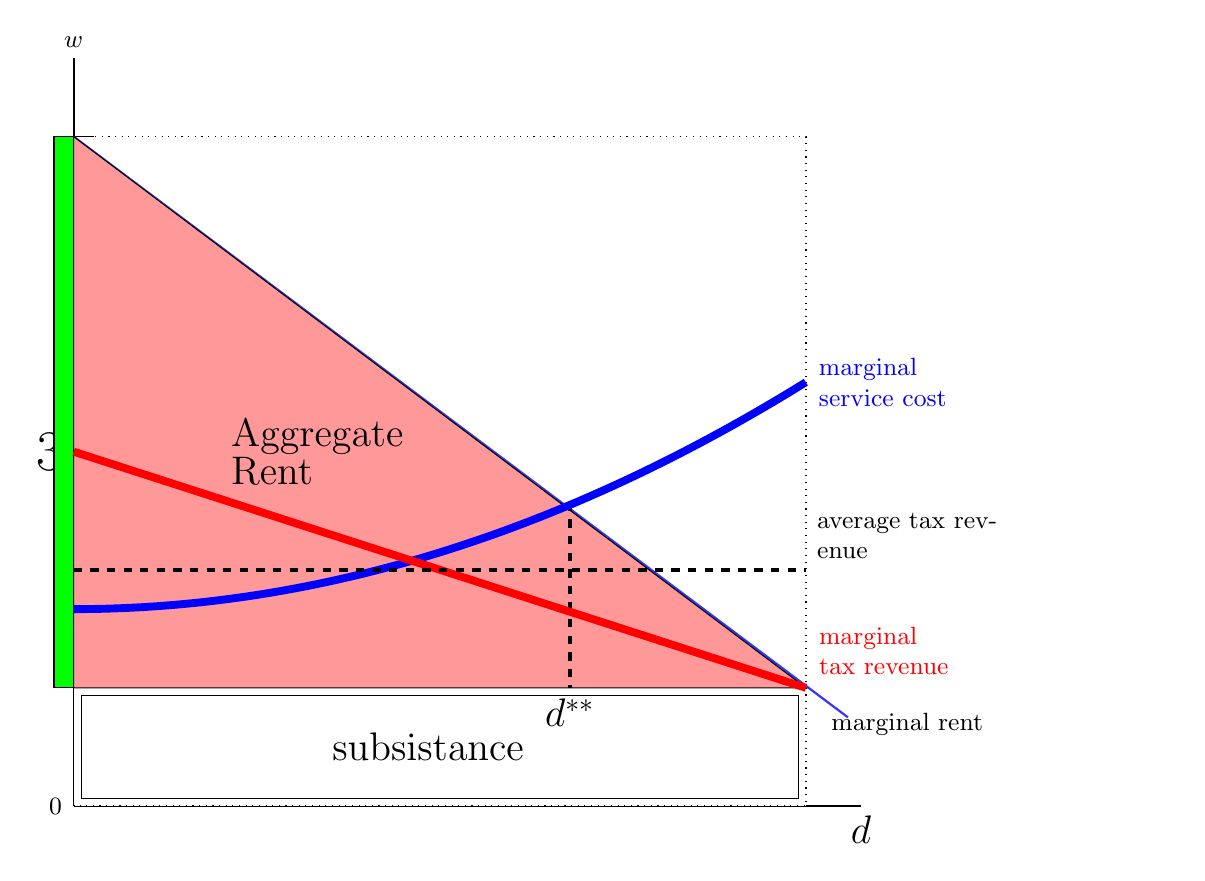
\begin{tikzpicture}[scale=1]
\def\bndmax{5}        %https://tex.stackexchange.com/questions/68462/filling-a-complex-region-with-tikz
\def\bndmin{0.2}
\def \n {8}  % height of y axis
\def \d {10}  % length  of x axis
\def \t {.75}  %  cost of transportation per unit x
\def \th {1}   %
\def \w {7}    %  wage premium
\def \om{1.5}%  omega =rural wage Zero for urban population
\def \azero{2}
\def \aprime {-.0}	
\tikzset{func/.style={thick,color=blue!80}}	
\draw [thick] (0,-\om) --(\d,-\om)node[below]{\Large$d$};  			% Zero for rural population
\draw [thick] (0,-\om)node[left=.5]{$0$} --(0,\n)node[above]{$w$};	% Y axis

%\draw [thick] (0,0)node[left=.5]{ subsistance}--(\d,0);
\node[left=.25] at (0,3){\huge $\omega$};
%\node[left=.25] at (0,\w+.3){subsistence plus};
%\node[left=.25] at (0,\w-.4){wage premium};	

\draw[fill=white, white] (0.1,-0.1) rectangle (14,-\om+.1);
\draw [fill=green] (-.25, 0) rectangle(.25, \w);
\node[right] at  (.25, \w/2){Added Productivity};
%\draw [ thick, ->](11.3,-\om/2)--(13, -\om/2)node [right] {\Large $d$};
\draw[fill=blue!40] (0.1,-0.1) rectangle (9.2,-\om+.1);


\draw[fill=black!0, dotted] (0,-\om) rectangle (9.30,\w);% new product repeat
\draw[func, domain=0:\w/\t+.5] plot [samples=200] (\x,{\w-\t*\x}); %rent profile
\draw[fill=blue!0] (0.1,-0.1) rectangle (9.2,-\om+.1);
\node at (4.5,-\om/2){\Large subsistance};
\draw[fill=red!40,] (0.,0.) -- (0,7)--(9.30,0.)--cycle;% Rent \w-.2
\node[text width=2cm] at (3.,3){\Large Aggregate \\Rent}; 		%Rent 
%\node at (5.8,5.7)[]{\Large Transportation};
\node at (6.3,4.8)[white]{\Large expenditure};
\draw[ line width=.5mm, dashed] (6.3,2.35)--(6.3,0)node[below ]{\Large$d^{**}$};

\draw[func, domain=0:9.3, line width=1mm,blue, text width=2cm] plot [samples=200] (\x,{1+\x^2/30})node[right]{marginal\\ service cost};
\draw[ line width=1mm, red] (0,3)--(9.3,0)node[above right, text width=3cm ]{marginal\\tax revenue};
\node at (9.5, -.2)[below right, text width=2cm]{marginal rent};

\draw[ line width=.5mm, dashed] (0,1.5)--(9.3,1.5)node[above right, text width=2.5cm ]{average tax revenue};

%GRID
%\draw[step=1cm,gray,very thin] (0,0) grid (10,10);

 \end{tikzpicture}


 
Two stylized facts should be noticed. The first is that the marginal cost of servicing generally  rises with the distance from the centre.  Figure
%~\ref{}
illustrates the general form of servicing costs, but not  the relative scales of rent and servicing costs. When this observation is combined with the `Henry George Theorem" () the conclusion is that the optimal size of the city  is at  $d^{**}$, where marginal service cost intersects with the marginal increase in total urban rent. 


The second stylized fact  is that property taxes, which are generally  fixed as a share of property value, decline as the distance from the centre increases.Figure %~\ref{} 
illustrates the general form of tax liabilities, although it does not  accurately represent their relationship top rent or  servicing costs.  This implies that in many or most urban situations the residents at the outer edges pay less than the average amount in property tax per unit of land, but cost  the community budget more than the average amount. In essence, the central city subsidizes the suburbs. (ref Perverse Cities)
This arrangement is both economically inefficient and unfair, but it has been built into the fiscal structure of cities largely as a result of automobile-based urban growth. It is likely that this fiscal misallocation saps some of the potential productivity growth of cities.

Both effects are more variable and than the simple model suggests.  One  conclusion urban theorists draw based on variants of the Alonzo model is that because property owners in the low-density urban margin are subsidized,  the subsidy is likely to create serious fiscal problems for municipalities in the long term and result in serious inefficiency in land use. 



\section{Class structure}\label{Sec:ClassStucture}

\begin{center}
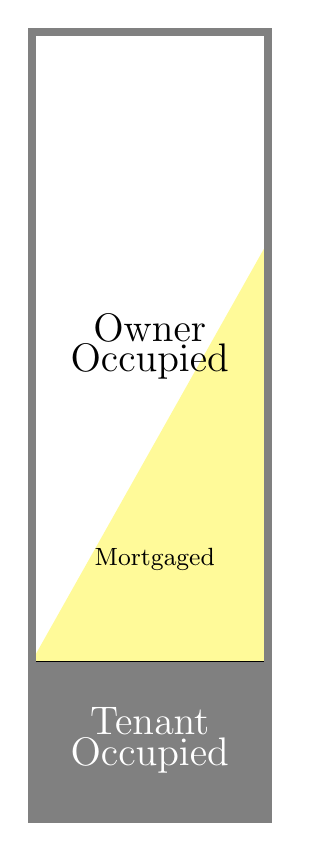
\begin{tikzpicture}{scale=.5}
%   \coordinate (planning) at (-5,1);%PREFACE
% \coordinate (economics) at (5,.75);%
%  \coordinate (geography) at (-.5,-2); %history
% \coordinate (finance) at (0,5); %  
\draw [fill=gray,] (0,0) rectangle (3,2); %TENANT
\draw [fill=yellow!40] (0,2)--(3,2)--(3,7.33); --cycle;% MORTGAGE %Calculation. 80\%owner, so  8 above the tenant line. 2/3*8=5.333. 5.333+2=
\draw[line width= 1mm, black!50] (0,0) rectangle (3,10);

\node at (1.5,6)
    [text width=2.4cm, align=center]
    {\baselineskip=20pt\Large Owner Occupied};
\node at (2,3.3)
    [text width=2.4cm]
    {\baselineskip=20pt Mortgaged};
\node at (1.5,1)
    [text width=2.4cm, align=center, white]
    {\baselineskip=20pt\Large Tenant Occupied};
\end{tikzpicture}
\end{center}

Figure: Housing Tenure 



At the stage illustrated in Figure~\ref{Fig:Rent1},  (Alonzo city suburbanized with owner occupiers) the model has three spatially segregated ``classes.'' Capitalists live in some spaceless utopia, urban workers commuting and earning wages $\omega + w$ reside in the urban commuter-shed and  %There may be a band surrounding the city or persons who do not commute but enjoy urban consumption amenities. 
\chapter{Financialization}

The focus of this thesis on a topic. that falls in the overlap  between least three academic  disciplines, Economics, Urban Geography, and Planning. The central and shared concern in this area is with geographic space.

Figure 1: The common concern of three fields
topic 
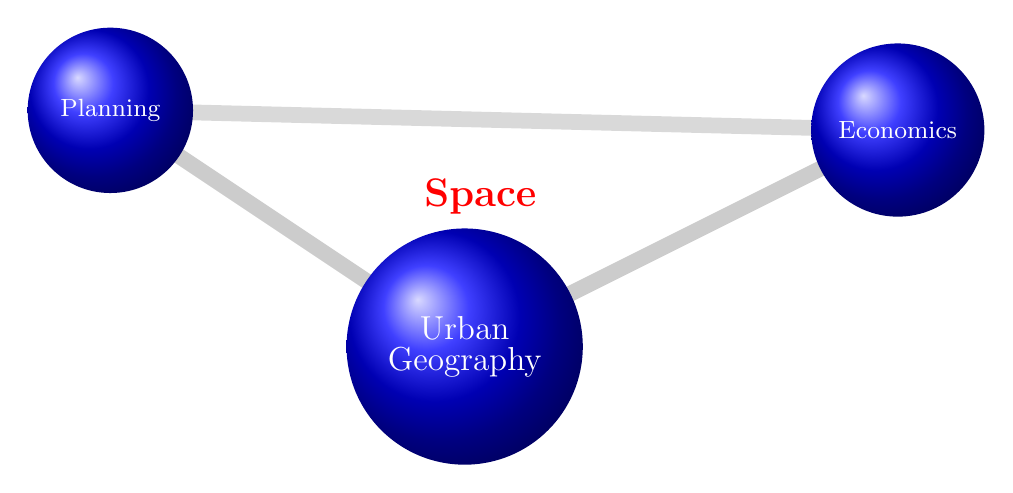
\begin{tikzpicture}{scale=.5}
% find color cotrol for ball. Tind way to stop line short of node
\coordinate (planning) at (-5,1);%PREFACE
\coordinate (economics) at (5,.75);%
 \coordinate (geography) at (-.5,-2); %history
\coordinate (finance) at (0,5); %

\draw [line width=2mm, black!15, ] (planning)--(economics);
\draw [line width=2mm, black!20, ] (geography)--(economics);
\draw [line width=2mm, black!20, ] (geography)--(planning);

%\draw [line width=2mm, black!25, ] (geography)--(finance);
%\draw [line width=2mm, black!20, ] (planning)--(finance);
%\draw [line width=2mm, black!20, ] (finance)--(economics);

\node [circle,shading=ball, minimum width=2.1   cm, white, align=center] (ball) at (planning) {Planning};
\node [circle,shading=ball, minimum width=2.2cm, white, align=center] (ball) at (economics) {Economics};
\node [circle,shading=ball, minimum width=3 . cm, white, align=center] (ball) at (geography)[text width=2cm] {\large Urban\\ Geography};

%\node [circle, shading=ball, minimum width=2.4cm, white, align=center] (ball) at (finance)[text width=2cm] {Finance};

\node at (-.3,-.1) [red] {\Large \textbf{Space}};
\end{tikzpicture}

A simple economic principle, the theory of rent, provides an organizing principle for the three disciplines. Rent theory has a long history in economics, going back to thinkers such as Richard Cantillon (1680s-1734), François Quesnay (1694–1774), the marquis de Mirabeau (1715–1789) and Anne-Robert-Jacques Turgot (name physiocrat) and Adam Smith (1723-1790) and received its classic statement in Ricardo (1772-1823). Nearly contemporaneous thinker, Johann Heinrich  von Th\"unen (1783-1850) developed a planning model to guide the location of economic activities for an urban-agricultural society.  A version of that model  was reinvented in urban geography by XXX. Alonzo\footnote{We use a version of the well-established model of Alonso (1964), Muth (1969) and Mills (1967), and formalised by Wheaton (1974),}

We link the Alonzo model with more recent work on growth theory starting with Robert Solo's XXX and with the endogenous growth models of Lucas () and draw on Jane Jacobs's insight that endogenous urban growth  is. now driving economic development. Jacobs's insight is empirically supported by recent work in the complexity literature on urban scaling by XXXX ()
\vspace{2cm}


Figure 2 with names

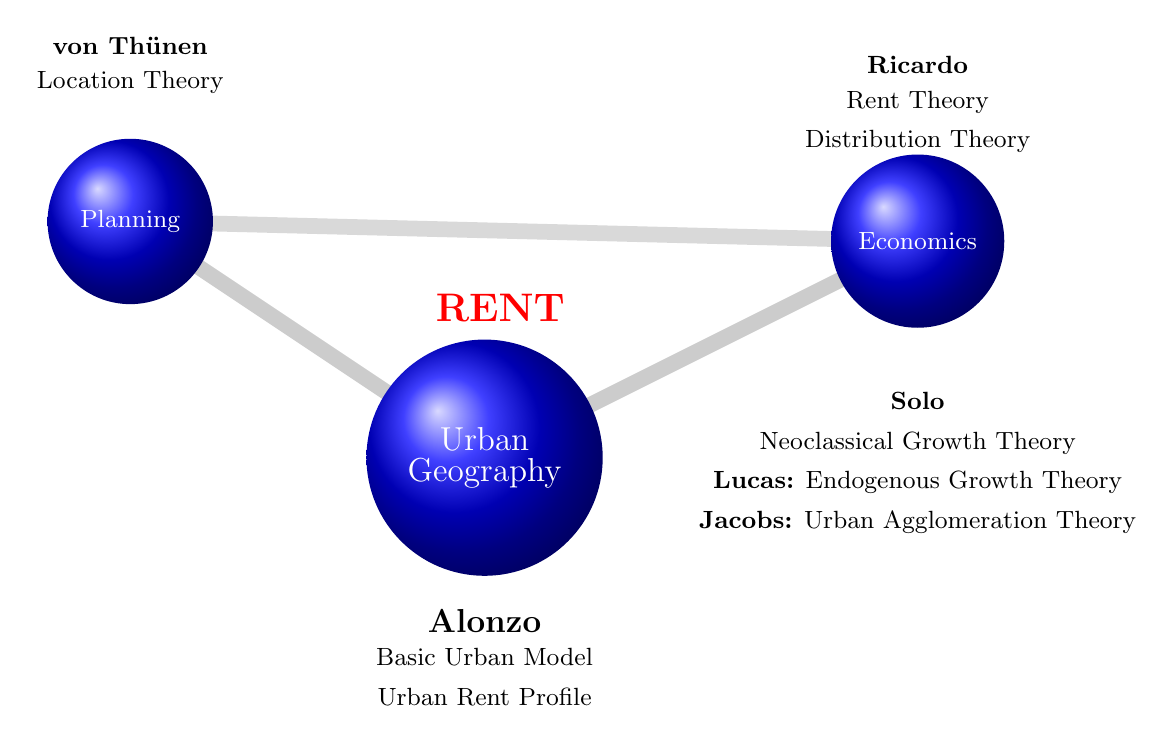
\begin{tikzpicture}{scale=.5}
% find color cotrol for ball. Tind way to stop line short of node
\coordinate (planning) at (-5,1);%PREFACE
\coordinate (economics) at (5,.75);%
 \coordinate (geography) at (-.5,-2); %history
\coordinate (finance) at (0,5); %

\draw [line width=2mm, black!15, ] (planning)--(economics);
\draw [line width=2mm, black!20, ] (geography)--(economics);
\draw [line width=2mm, black!20, ] (geography)--(planning);

%\draw [line width=2mm, black!25, ] (geography)--(finance);
%\draw [line width=2mm, black!20, ] (planning)--(finance);
%\draw [line width=2mm, black!20, ] (finance)--(economics);

\node [circle,shading=ball, minimum width=2.1   cm, white, align=center] (ball) at (planning) {Planning};
\node [circle,shading=ball, minimum width=2.2cm, white, align=center] (ball) at (economics) {Economics};
\node [circle,shading=ball, minimum width=3 . cm, white, align=center] (ball) at (geography)[text width=2cm] {\large Urban\\ Geography};

%\node [circle, shading=ball, minimum width=2.4cm, white, align=center] (ball) at (finance)[text width=2cm] {Finance};

\node at (-.3,-.1) [red] {\Large \textbf{RENT}};

% new stuff
\node at (planning) [above=2cm] {\textbf{von Th\"unen}};
\node at (planning) [above=1.5cm] {Location Theory};

\node at (economics) [above=2cm] {\textbf{Ricardo}};
\node at (economics) [above=1.5cm] {Rent Theory};
\node at (economics) [above=1.0cm] {Distribution Theory};

\node at (economics) [below=1.8cm] {\textbf{Solo}};
\node at (economics) [below=2.3cm] {Neoclassical Growth Theory};
\node at (economics) [below=2.8cm] {\textbf{Lucas:} Endogenous Growth Theory};
\node at (economics) [below=3.3cm] {\textbf{Jacobs:} Urban Agglomeration Theory};


\node at (geography) [below=1.8cm] {\textbf{\large Alonzo}};
\node at (geography) [below=2.3cm] {Basic Urban Model};
\node at (geography) [below=2.8cm] {Urban Rent Profile};
\end{tikzpicture}

Labasis of the wealy and pokliticval poiwer of nd rent was historically the 

Figure 3: space and value

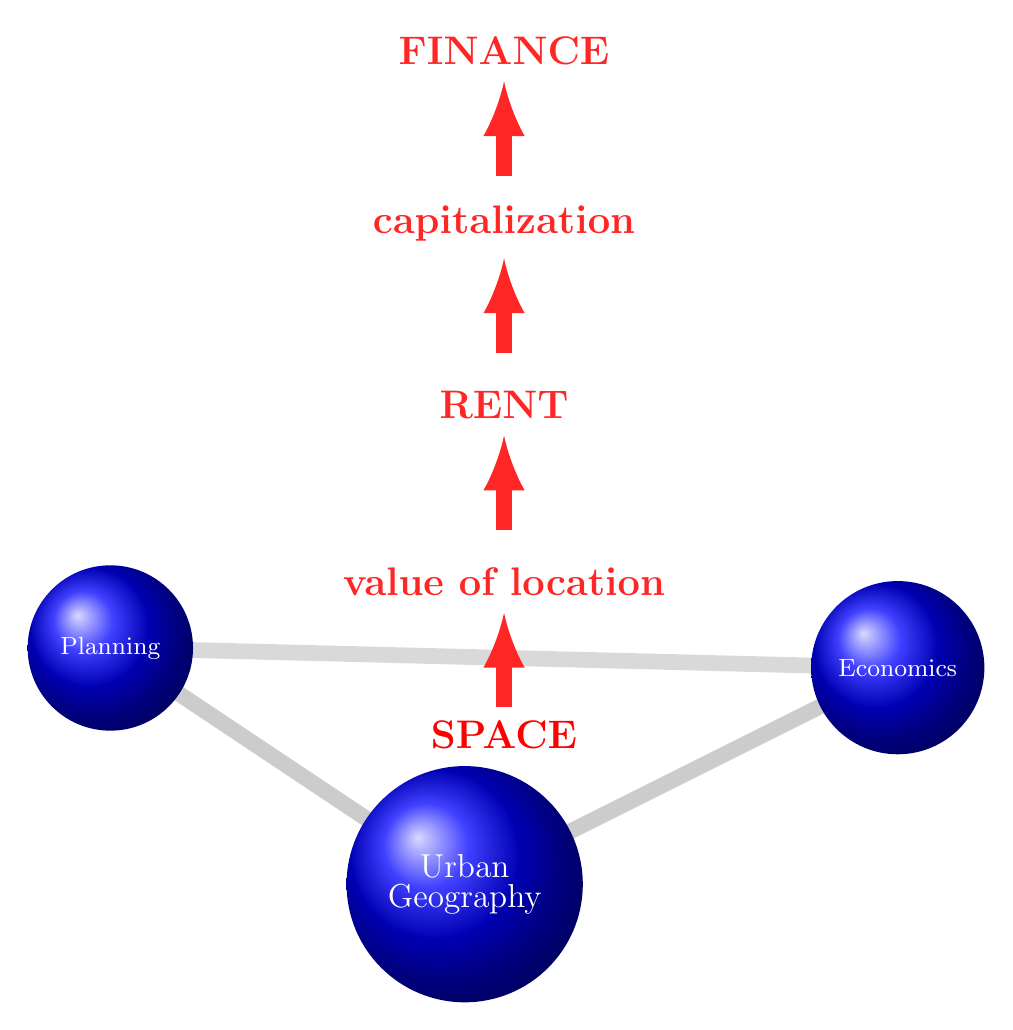
\begin{tikzpicture}{scale=.5}
% find color cotrol for ball. Tind way to stop line short of node
\coordinate (planning) at (-5,1);%PREFACE
\coordinate (economics) at (5,.75);%
 \coordinate (geography) at (-.5,-2); %history
\coordinate (finance) at (0,5); %

\draw [line width=2mm, black!15, ] (planning)--(economics);
\draw [line width=2mm, black!20, ] (geography)--(economics);
\draw [line width=2mm, black!20, ] (geography)--(planning);

%\draw [line width=2mm, black!25, ] (geography)--(finance);
%\draw [line width=2mm, black!20, ] (planning)--(finance);
%\draw [line width=2mm, black!20, ] (finance)--(economics);

\node [circle,shading=ball, minimum width=2.1   cm, white, align=center] (ball) at (planning) {Planning};
\node [circle,shading=ball, minimum width=2.2cm, white, align=center] (ball) at (economics) {Economics};
\node [circle,shading=ball, minimum width=3 . cm, white, align=center] (ball) at (geography)[text width=2cm] {\large Urban\\ Geography};

%\node [circle, shading=ball, minimum width=2.4cm, white, align=center] (ball) at (finance)[text width=2cm] {Finance};
\draw [line width=2mm, red!85, -latex ] (0, 7)--++(0,1.2)node[above=-.1] {\Large \textbf{FINANCE}};
\draw [line width=2mm, red!85, -latex ] (0, 4.75)--++(0,1.2)node[above=-.1] {\Large \textbf{capitalization}};
\draw [line width=2mm, red!85, -latex ] (0, 2.5)--++(0,1.2)node[above=-.1] {\Large \textbf{RENT}};
\draw [line width=2mm, red!85, -latex ] (0, .25)--++(0,1.2)node[above=-.1] {\Large \textbf{value of location}};
\node at (0,-.1) [red] {\Large \textbf{SPACE}};
\end{tikzpicture}



We further link the model of urban rents to emerging concerns about the financialization of the housing market. The key insight we offer is that the financialization  of the housing sector is a  form of rent-seeking that must have detrimental effects on urban development and on the well-being of urban residents.


\vspace {2cm}
Figure 4 with finance

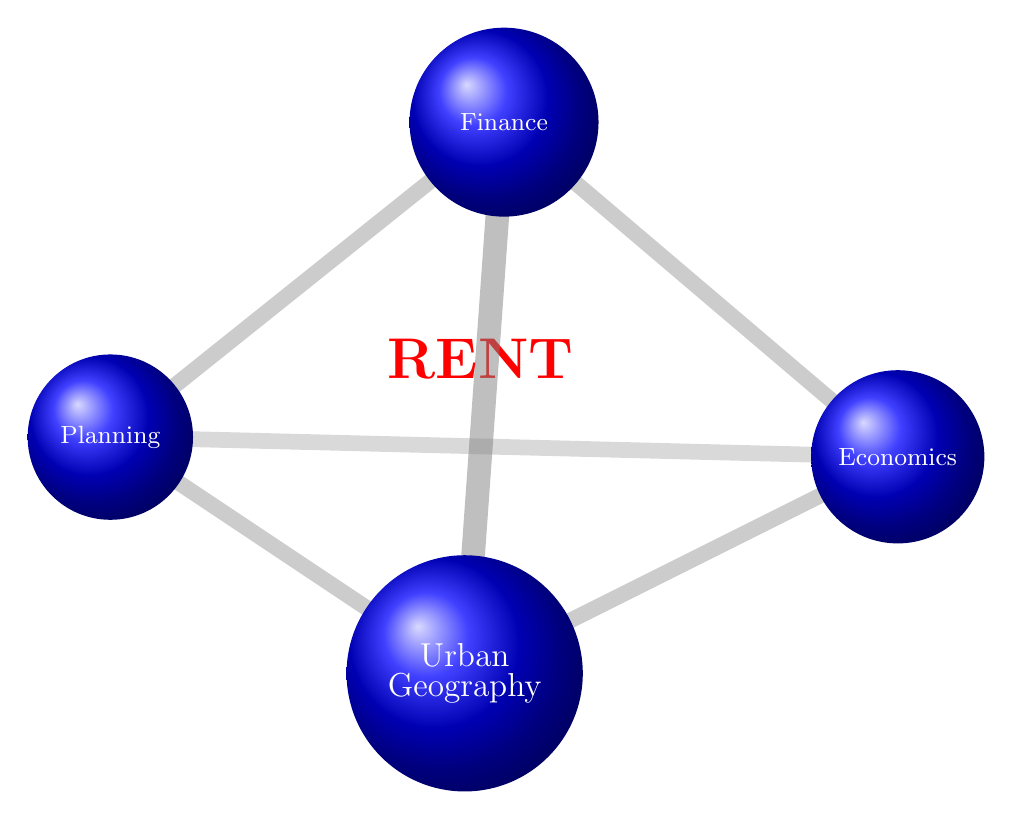
\begin{tikzpicture}{scale=.5}
% find color cotrol for ball. Tind way to stop line short of node
\coordinate (planning) at (-5,1);%PREFACE
\coordinate (economics) at (5,.75);%
 \coordinate (geography) at (-.5,-2); %history
\coordinate (finance) at (0,5); %

\draw [line width=2mm, black!15, ] (planning)--(economics);
\draw [line width=2mm, black!20, ] (geography)--(economics);
\draw [line width=2mm, black!20, ] (geography)--(planning);

\node at (-.3,2) [red] {\huge \textbf{RENT}};

\draw [line width=3mm,  black!50,opacity=.5 ] (geography)--(finance);
\draw [line width=2mm, black!20, ] (planning)--(finance);
\draw [line width=2mm, black!20, ] (finance)--(economics);

\node [circle,shading=ball, minimum width=2.1   cm, white, align=center] (ball) at (planning) {Planning};
\node [circle,shading=ball, minimum width=2.2cm, white, align=center] (ball) at (economics) {Economics};
\node [circle,shading=ball, minimum width=3 . cm, white, align=center] (ball) at (geography)[text width=2cm] {\large Urban\\ Geography};

\node [circle, shading=ball, minimum width=2.4cm, white, align=center] (ball) at (finance)[text width=2cm] {Finance};


\end{tikzpicture}


\vspace {2cm}
Figure 4 with finance

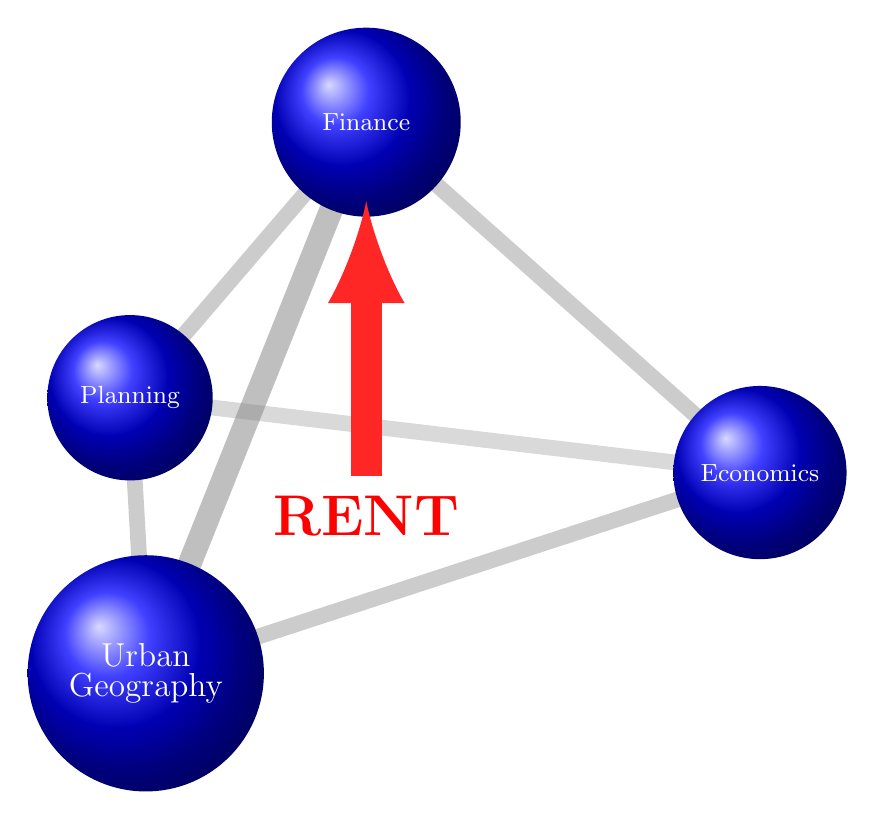
\begin{tikzpicture}{scale=.5}
% find color cotrol for ball. Tind way to stop line short of node
\coordinate (planning) at (-3,1.5);%PREFACE
\coordinate (economics) at (5,.55);%
 \coordinate (geography) at (-2.8,-2); %history
\coordinate (finance) at (0,5); %

\draw [line width=2mm, black!15, ] (planning)--(economics);
\draw [line width=2mm, black!20, ] (geography)--(economics);
\draw [line width=2mm, black!20, ] (geography)--(planning);

\node at (.0,0) [red] {\huge \textbf{RENT}};

\draw [line width=3mm,  black!50,opacity=.5 ] (geography)--(finance);
\draw [line width=2mm, black!20, ] (planning)--(finance);
\draw [line width=2mm, black!20, ] (finance)--(economics);

\node [circle,shading=ball, minimum width=2.1   cm, white, align=center] (ball) at (planning) {Planning};
\node [circle,shading=ball, minimum width=2.2cm, white, align=center] (ball) at (economics) {Economics};
\node [circle,shading=ball, minimum width=3 . cm, white, align=center] (ball) at (geography)[text width=2cm] {\large Urban\\ Geography};

\node [circle, shading=ball, minimum width=2.4cm, white, align=center] (ball) at (finance)[text width=2cm] {Finance};
\draw [line width=4mm, red!85, -latex ] (0, .5)--(0,4);


\end{tikzpicture}



\vspace{2cm}

\section{Financialization and Urban Land Rents}
%BASED ON Financialization_of_the_Housing_Market.tex

Financialization is the process by which financial institutions, markets, etc., increase in size and influence. More specifically it is the process by which future streams of revenue and speculative gains are systematically captured by individuals and institutions with financial assets. Financialization of the housing market is the increasing control of the stock of urban land and housing in order to capture the scarcity rent generated by the people of the city.  

Mortgages, for example, are a financial instrument that allows lenders to  participate in housing purchases in the present in exchange for a future flow of payments.  The mortgage does not create housing, but it enables the prospective buyer to become the nominal owner of an asset that produces a stream of benefits. The stream of benefits from secure housing near a source of income generally greatly exceeds a buyer's current assets. The mortgage enables the  transfer of ownership because it makes it possible to transfer the rights to the future income of the buyer to the mortgage holder who then, in effect, is the actual owner until the terms of the mortgage are fulfilled.  If the mortgagee fails make those payments the mortgage holder  takes over the asset. 

The mortgage itself is both an financial instrument that enables a purchase and a financial asset that can be bought and sold. When we consider urban housing, it is the right to future income generated by capital, labour and the the city itself through the agglomeration effects that drive productivity. It is an instrument that indirectly captures a share of the urban rents. As productivity rises, wages rise, rents rise, property prices rise and mortgages rise. 

About 80\% of Canadian homes are owner-occupied and about a third of the  value of the homes is held as mortgages. Approximately two-thirds of the net land rents associated with housing therefore accrue to owner occupiers. {\color {red}CHECK THESE NUMBERS } 

For urban theory and policy formation it is important to distinguish between financial instruments that enable production of real assets and instruments like the mortgage that facilitate the transfer of real assets. Housing developers borrow to purchase land for development and builders borrow to finance construction. While important, the financial instruments involved are not driving the financialization of housing.  The size of the loans involved is affected by the amount of land purchased and the potential rents earned by that land, the degree of non-occupant ownership is not affected.






  a productive asset is acquired as a financial asset it remans productive. %African land or land in Northern Ontario acquired by holding companies may even be made more productive. 
The goal of such investments, however, is generally to achieve a capital gain over time. Financial analysis is essentially about rates of return on financial capital invested. The opportunity for capital gains  attracts financial capital to the housing market.%Financial managers have no interest is n in assets that are not expected to increase in value. 
\footnote{.} 

Financialization of urban housing benefits  a globally distributed rentier class of urban landholders. We will make this more explicit below the incentive structure deriving the further financialization of the housing market.

\section{Literature on theory and evidence}
{\color{red}There is substantial evidence that the financialization of urban housing is underway in Canadain cities

PROVIDE EVIDENCE 	mention theories?}


Two questions arise when we observe growing participation of global capital in the urban housing system: 
\begin{enumerate}
\item How far will the financialization of urban land go? 
\item That are the implications for the urban economy and the welfare of the urban population? 
\end{enumerate}

We can demonstrate  that  in the absence of policy interventions, differential access to finance capital ensures that capital owners acquire an increasing share of urban land over time and capture the growing  land rents  from urban productivity growth. Growing wealth inequality emerges within a simple, widely accepted model of the urban land market. In the limit,  urban residents are tenants, and new residents  without capital do  not receive any of the increases in rents arising from the growing productivity of the city. 

%The first question therefore is reduced to which capital holders will increase their share of urban land and whether there is any reason to expect the process of financialization process to stop or reverse itself.




\section{The incentives for financialization}%\label{Sec:RentAndClass}

  

%Instead, drawing on the ideas of Jane Jacobs, Lucas proposes the city as the unit of analysis .Lucas, Robert (1990), "Why Doesn't Capital Flow from Rich to Poor Countries?," American Economic Review Papers and Proceedings v. 80, no. 2 (May) pp. 92-96.  
%Jacobs, Jane  (1969), The Economy of Cities (New York: Random House).  
% The Death and Life of Great American Cities \cite{Jacobs61}




\section{The rate of return on a property purchase}


ADD TABLE WITH VARIABLE DEFINITIONS
 
 In this section we develop a model of the return to investment in urban housing/land. We'll assume that all agents are speculating on potential capital gains as well as on the use values they get from a property.  We will also assume that the use value is captured by the stream of rental values, whether a home is owner occupied or  held by an investor as a financial asset. To keep the analysis simple without loss of generality we will consider a one-period investment.
 
 The speculator  invests a down payment, $D$, and gets back at time $T$ the  increased price $(1+\dot p)P_0$, plus rents, minus any costs and minus the mortgage with interest.\footnote{We have applied this model to explore the effect of a vacancy tax in Beirut.  Fort that analysis we  added a use-value, $U$ in place of rent for expatriate owners to represent using the property - say one month a year - when they are not renting the property and a \textbf{vacancy tax}, $T$ at rate $t$ to affect the speculator's  decision. \cite{Al-Shihabi}}


\begin{eqnarray*}
V  	&=& capital\ gain - Interest\ due  	+ Rent  - operating\ cost -taxes\\
% 	&=& \delta P_T-D \qquad \qquad \quad - (1+\delta r)M \quad	 + R  	-C\\
% 	&=& \delta P _T \qquad-(P_0-M) \quad- (1+\delta r)M 	 + R  	-C\\
%	&=& \delta (1+\dot p)  P_0 -(P_O -M)  -(1+\delta r)mP_0  + R  -C\\
%	&=& \delta (1+\dot p)  P_0 -P_O + M \qquad -(1+\delta r)mP_0  + R -C\\
%	&=&( \delta (1+\dot p)-1)  P_0  + mP_0 \quad -(1+ \delta r)mP_0  + (\rho-\kappa)P_0\\	
%	&=& \left(  \delta (1+\dot p)-1    + m \quad - m(1+\delta r)  + (\rho-\kappa)\right)P_0\\'
%	&=& \left(  \delta (1+\dot p)-1    + m \quad - m-\delta rm  + (\rho-\kappa)\right)P_0\\
&=& \delta(P_T- (1+r)M) \qquad \qquad 	 + R  	-C   - T\\
&=& \delta((1+\dot p)  P_0- (1+r)mP_0)   + \rho P_0  	-\kappa P_0 - tP_0\\
&=&( \delta((1+\dot p)  - (1+r)m) \ + \rho   	-\kappa -t) P_0
\end{eqnarray*}

This is the  net present value of buying, and selling after one period. It has  6 exogenous parameters, $\delta, \dot p, r, m, \rho, \kappa$ and $t$.   Operating revenue and costs $\rho, \kappa$ and $t$ are expressed as  present values. Both the  share of the price  that can be mortgaged, $m$, and the interest rate  and $r$ are functions of the agent's wealth. $\delta$ may be correlated with wealth as well. 

The rate of return $v$ is the value of the gain, $V$, divided by  the size of the downpayment, $D$. 
%The rate of return is $v = \frac{V}{D}$. %For expat investors, we get a \textbf{decision rule}:\begin{enumerate}
%\item  if $v \geq a$ (with some private use?) with no rent,  don't bother renting. 
%\item If $v(no\ rent\ and\ tax) < a\geq v(with\ rent)$,  then  rent. 
%\item If $ v(with\ rent) \le a $,  then sell 
%\end{enumerate}\
\begin{eqnarray}
v&=&( \delta((1+\dot p)  - (1+r)m) \ + \rho   	-\kappa - t ) \frac{P_0}{D}   \nonumber\\
		&=&( \delta((1+\dot p)  - (1+r)m) \ + \rho   	-\kappa - t ) \frac{P_0}{P_0-mP_0}   \nonumber\\
		&=&\frac{ \delta(1+\dot p  - (1+r)m) \ + \rho   	-\kappa - t } {1-m} \label{Eqn:DecisionRule}
\end{eqnarray}






%%%%%%%%  VVVVVVVVVVVVVVVVVVVVVVV   This section May 18 to cut?  V
%%%%%%%%  ^^^^^^^^^^^^^^^^^^^^^^^^^^^^^^^  This section May 18 to cut?  V

%\begin{enumerate}
%
%\item  the buyer and seller calculate the value of the property  differently. 
%
%\item  the  buyer and seller may have different expectations of the path of prices and therefore the stream of rents.
%%There are two standard ways that expectations are modelled
%%	\begin{enumerate}
%%	\item \textbf{Adaptive expectations.} Expectations are largely based on what has happened in the past. 
%%	Under normal conditions most people people have relatively weak incentive to get forecasts about inflation correct, and lack the resources and time to purchase expert advice. 
%%	Recent price trends are easily available and likely to be the main source of  information.
%%	\item     \textbf{Rational expectations.} Expectations are based on a model of the future economy. 
%%International investors and banks employ economists and other experts to  forecast prices, exchange rates, and trends in the economy.
%%	\end{enumerate} 
%\end{enumerate}
% Why would  discount rates differ between identical workers? Buyers and sellers are not identical in wealth, obviously. 
%%We could implement the first  explanation either by generating expectational errors based on functional class or wealth. 

%As expected
%\begin{enumerate}
%\item A large $m$ magnifies the return. (downpayment is smaller)
%\item A lower mortgage interest rate increases the return because of interest on the mortgage
%\item A lower discount rate $\delta$ reduces the subjective rate of return
%\item Higher expected price appreciation increases the attractiveness of investment
%\item Higher rents makes the unit more profitable if rents are being collected
%\item Lower costs increase profits
%\item Lower tax rates decrease holding costs and increase the value of the investment
%\end{enumerate}
The implications of Equation~\ref{Eqn:DecisionRule} are significant for the evolution of the urban land market and class structure. They suggest strongly that large wealth-holders will get higher expected and actual rates of return on land than those with  lower wealth holdings,\footnote{Case and Schiller ``%The ratio of construction costs to price, changes in adult population and
 ... increases in real per capita income all are positively related to excess returns or price changes over the subsequent year.''} and that the managers of large pools of capital will have an even greater advantage. 
 
 Make list of effects variable by variable. describe derivatives
 
Consistent with the empirical evidence, net returns for investment are increasing with wealth. 
%
%\begin{enumerate}
%\item Given the  common rule that mortgage payments cannot exceed some fraction of disposable income, the wealthy will be able borrow larger amounts and at lower interest rates that the less wealthy. At any distance from the centre they will be able to make a higher bid.
%
%\item The cost of capital is known to differ for rich and poor. Say, for example, the cost of borrowing, $r_i$ for agent $i$ if the base lending rate is $\bar{r}$
% \[ r_i = (A + B \frac{\bar{W}}{W_i})\bar r\]
%where $\bar{W}$ is mean wealth and $W_i$ is individual wealth. Figure~\ref{Fig:BorrowingCost} illustrates the effect.\footnote{Fr\'ed\'erick Demers found that the response of housing investment to interest rates has become more pronounced over time. Modelling and Forecasting Housing Investment: The Case of Canada,  Research Department, Bank of Canada, Ottawa, Ontario, Canada K1A 0G9 fdemers@bankofcanada.ca} 
%
%\begin{figure}[htbp]
%\begin{center}
%\chapter{SAPriceOfCapital}

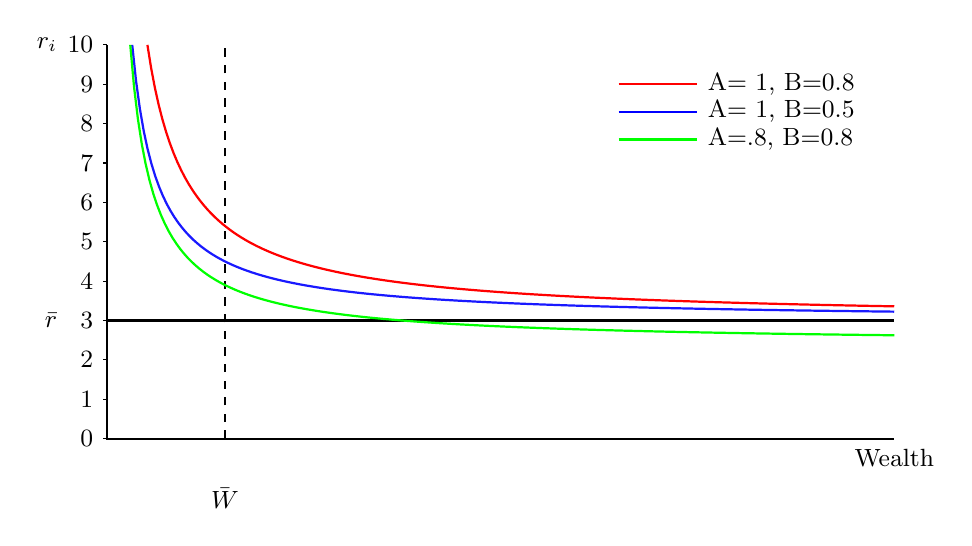
\begin{tikzpicture}[scale=.5]
%\def\bndmax{5}        %https://tex.stackexchange.com/questions/68462/filling-a-complex-region-with-tikz
%\def\bndmin{0.2}
\def \Y {10}  % height of y axis pecent
\def \W {20}  % length  of x axis
\def \Wbar {3} % jmeam wealth
\def \omega {3}
\def \A {1}  %was .5
\def \B {.5}
%Equation   \[ r_i = (A + .5 \frac{\bar{W}}{W_i})\omega\]
\def \Wmin{.63}  %This sets the lower limit fo the 
\def \Wmin{(\B*\Wbar)/(\Y/\omega-\A)} %function to keep in in bounds
	
\tikzset{func/.style={thick,color=blue!90}}	

\draw [thick] (0,\Y)node[left=.5cm]{$r_i$} -- (0,0)--(\W,0)node[below]{Wealth};  	% Axes
\draw [thick] (0,\omega)node[left=.5cm]{$\bar r$} -- (\W,\omega);  	% Axes
\draw [thick,dashed] ( \Wbar,0)node[below=.5cm]{$\bar{W}$} -- (\Wbar,\Y);  	% Axes

\foreach \yi in {0,...,\Y} \draw (0,\yi)--(-.1,\yi)node[left]{\small$\yi$};

\draw[func,domain=\Wmin:\W] plot [samples=200] (\x,{(\A+\B*\Wbar/\x)*\omega});
\def \A {.8}
\draw[func,domain=\Wmin:\W, green] plot [samples=200] (\x,{(\A+\B*\Wbar/\x)*\omega});

\def \A {1}
\def \B {.8}
\draw[func,domain=\Wmin:\W, red] plot [samples=200] (\x,{(\A+\B*\Wbar/\x)*\omega});

\draw [red,  thick](13, 9)--(15,9)node [right, black] {\small A=\ 1,\ B=0.8};
\draw [blue,  thick](13, 8.3)--(15,8.3)node [right, black] {\small A=\ 1,\ B=0.5};
\draw [green, thick](13, 7.6)--(15,7.6)node [right, black] {\small A=.8, B=0.8};
 \end{tikzpicture}
% Figure of cost of borrowing
%\caption{Borrowing cost for  $A=1$  $B=0.5$ (blue);  $A=1$  $B=0.8$ (red);  $A=.8$  $B=0.8$ (green);}
%%\caption{Hypothetical wealth-dependent borrowing cost}
%\label{Fig:BorrowingCost}
%\end{center}
%\end{figure}%
%
%\item If agents discount at their borrowing rate, wealthier agents may have a lower subjective rate of time preference and therefore value properties more highly. 
%\end{enumerate}

The implication is that those with more capital will be at an advantage in the urban housing  market. Tax treatment of income and capital gains as well as interest deductability will influence Equation~\ref{Eqn:DecisionRule}'s strength and who benefits most. 

There are some additional implications

%\begin{enumerate}
%\item  expecting greater price appreciation raises expected profitability. The wealthy and financial corporations  are likely to have better price forecasts than  the occasional home buyer.
%\item higher expected  rents may result from expecting greater price appreciation raises expected profitability or greater willingness to raise rents for tenants
%\item There may be scale economies in maintenance  of rented housing
%\item There may be opportunities to shelter income with land held for investment (speculative) purposes
%\end{enumerate}

These items suggest that financial corporations may have advantages relative to individual investors. Combined with better access to capital and interest deductability, it is reasonable to expect that financial corporations, which essentially pool the purchasing power of wealth holders, increasingly dominate urban land markets. %A recent report claimed 15\% of Tioron0's land transa

In the limit it appears that wage income will never be sufficient to support home ownership in growing cities. 
Overall, this suggests rising housing prices are not a bubble because speculation decouples use-value from price setting. %


These observations about  the rate of return on urban capital raise a set of very interesting issues.  


\begin{itemize}
\item The effect of increasing the urban workforce is to increase the marginal products of  both capital and labour throughout the urban economy. This premium on production in cities is positive when $\Lambda'$ is greater than zero.
 \item  As long as $\Lambda'>0$ cities will  grow, potentially leading to the ``catastrophic agglomeration''  that has been noted in other models.  %(\cite{FujitaKrugmanVenables, BaldwinMartin, Krugman1991, Gurwitz2019}).  City size could be bounded, in which case the city system would grow by increasing the number of cities. This appears to depend on the model features and parameters. 
\item Cities will draw investment away from rural and remote areas.
\item Cities will draw labour away from rural and remote areas. 
\item Even in competitive markets capital captures  scale benefits until an entry equilibrium is achieved.
\item Landowners  capture the agglomeration benefits that are not dissipated in transportation costs.
\end{itemize}

These appear to be features of the economy we observe.


\section{The long-run evolution of complex urban systems}

It is clear that cities city systems and city economies are complex systems. Complex systems are sensitive to scale and tend to generate emergent properties over time. In the history of cities we discern a series of transitions arising out of growing size and complexity. There is no reason to  think that evolution has stopped. In fact our analysis has focussed on a significant transition that is currently underway. The transformation of cities as humans become an urban species has had a series of stages, each of which was tied to production technologies and largely determined social relations of the period.

Early cities were built on 
 




DOES THIS GO TO THE MODEL CHAPTER?

The model is we employ consistent with the theories of Ricardo and Henry George in locating the ground of urban exploitation and class in the capacity to extract social surplus through land ownership, and differs from the standard Marxian analysis in its reliance on access to financial capital rather than control of productive physical capital. The paper concludes that given existing land ownership patterns which encourage speculative investment, housing prices must rise and income inequality must increase. 



We  incorporate Jacobs-style agglomeration economies (\cite{Beaudry:2009ua, Panne:2004vb, JacobsEofC})  similar to the way the  Solo-Swan model incorporates  labour-augmenting technical change using a simple Cobb-Douglas production function.  We bypass the complexity of modelling firms  by allowing population increases  to directly increase urban wage premium.\footnote{The transmission of productivity increases arising from agglomeration effects  to the urban wage through firms, can be modelled in many ways. The agglomeration effects are external to the firm and therefore likely to be unexpected. If  firms underestimate the marginal product of labour, labour productivity will be greater than expected, output will be higher than planned output, and revenue and profits will therefore be higher than expected. Excess demand will attract more productive capital which in turn will demand more labour,  Rising labour demand drives up the wage. The agglomeration effect driving growth is essentially a public good in which individual firms will under-invest. This raises an policy challenge that we leave for others.} %, It is straightforward to compute the rate of excess return for  this model. 
%We insert the production function  into a standard Alonso-style model of a city economy (\cite{Alonso64}). 
In the background, individual firms have decreasing returns, but the presence of agglomeration economies external to firms but internal to the city gives the urban economy as a whole increasing returns to scale. \footnote{These effects can be large. Irwin and Klenow  studied learning in chip production focusing  on the key issue of spillovers. They found learning rates of 10 to 27 per cent, averaging 20 per cent. They indicated that a good part of learning is internal, and that national spillovers were no greater than international spillovers. "... a firm learns three times as much from an additional unit of its own cumulative output as from another firm's cumulative output, regardless of the other firm's country of location. However, rest-of-world cumulative production is typically more than three times any given firm's cumulative production. This means that the absolute contribution of world cumulative production to each firm's experience outweighs the absolute contribution of its own cumulative production. In this sense, spillovers are substantial." (pp. 1217-1218).} 


Rural producers in our model pay a constant wage $\omega$. This is a convenient simplification, not a necessary feature of the model. The urban production sector pays a wage premium $w$.\footnote{
HirschWage (a citation) observe that, ``Following GlaeserMare (a citation),  a  large  empirical  literature  has  investigated differences in wages across labor markets of different sizes. The general finding of this literature is that a significant urban wage premium exists. and that this premium consists both of a level effect and a growth effect that arises as workers gain urban work experience''. } As in the standard circular city model the constraint on growth is provided by transportation costs, which limits the size of the commuter-shed and therefore the labour force at any wage. 




 
 \begin{tikzpicture}%[scale=.8]
    \tikzstyle{every node}=[font=\small]
%\draw[help lines,step=.5] (0,-11) grid (11,11);

\coordinate (aa) at (-1.5,7.5);%PREFACE
\coordinate (a) at (-1,10);%
 \coordinate (b) at (1.5,7); %history
\coordinate (c) at (6,10); %
\coordinate (d) at (9,9);%
\coordinate (ee) at (-4,7);%
  \coordinate (e) at (-1.5,5); %Community label
\coordinate (f) at (9.5,7.7); %???    PLAN
\coordinate (g) at (9,5); %Economics label
\coordinate (h) at (4.5,7);%tenure
\coordinate (ii) at (-4,4);%
   \coordinate (i) at (1,4);  
\coordinate (j) at (3,3.5);%whatis
\coordinate (k) at (6,4);%
 \coordinate (l) at (6.5,3.5);%joint
\coordinate (mm) at (-1.9,1);%coops
 \coordinate (m) at (1,1);%community grey circle
  \coordinate (n) at (3,1); %
  \coordinate (o) at (9.5,1); %efficiency
				 \coordinate (oo) at (6.5,1);%
				  \coordinate (o1) at (10.7,2);	 \coordinate (o2) at (10.7,0);%Propositions
\coordinate (p) at (9,-1.5);%externalities
				
\coordinate (qq) at (-4,-2);
\coordinate (q) at (-1,-1);%innovation
 \coordinate (r) at (3.2,1.2);%trans
  \coordinate (s) at (3.2,-1.2);%capital
 \coordinate (t) at (6.5,-2);%pubgoods
\coordinate (AA) at (-2,-5);%
 \coordinate (A) at (1,-5);%
\coordinate (B) at (3.7,-4); %
\coordinate (C) at (4.2,-4);%forestryEC
\coordinate (D) at (-1,3);%foresters
\coordinate (EE) at (-1,-8); \coordinate (E) at (1,-8); \coordinate (F) at (3,-8); \coordinate (G) at (6,-8); \coordinate (H) at (10,-4);%Policy
\coordinate (II) at (-4,-11);  \coordinate (I) at (1,-11); \coordinate (J) at (3,-11); \coordinate (K) at (6,-11); \coordinate (L) at (10,-11);
%\coordinate (M) at (coordinate); \coordinate (N) at (coordinate); \coordinate (O) at (coordinate); \coordinate (P) at (coordinate);
%\coordinate (Q) at (coordinate); \coordinate (R) at (coordinate); \coordinate (S) at (coordinate); \coordinate (T) at (coordinate);
% \fill[red, fill opacity=.8] (0,0) circle (4cm);
\fill [gray, fill opacity=0.2] (m) node [text width=2cm, black, opacity=1] 				(community)	{} circle (3cm);
\fill [gray, fill opacity=0.1] (oo)  node [text width=2cm, align=left, black, opacity=1] 		(econ) {} circle (3.5cm);
\node at (e) [ ] 		(comLtabel) {COMMUNITY};
\node at (g) [ ] 		(ecLabel) {ECONOMICS};
				%\draw (0,3.2,1) node [text width=1.5cm, text centered] {$Economics$};
			%\draw [fill=red, fill opacity=0.3]  (aa) node [ text width=2cm, black, opacity=1] 									(preface)		{PREFACE: Why, claims} circle (1.4cm);
\node [circle, draw,  fill=gray, opacity=.5,, text width=1.5cm] at			 (aa) 		(preface)		{PREFACE};
\node [] at			 (f) 		(plan)		{\Huge PLAN};
			%\draw [fill=blue, fill opacity=0.35] (b)node [text width=2cm, align=center, black, opacity=1] 			(history){History: New is Old} circle (1.2cm);
\node[circle, draw, text width=1cm, align=center, black, opacity=1]at 	(b)(history){History} ;
			%\draw [fill=pink, fill opacity=0.5] 		(h) node [text width=2cm, black, opacity=1] 								(tenure) 	{\color{black}tenure} circle (1.2cm);
\node[circle, draw,  text width=1cm, align=center, black] at 				(h) (tenure) 	{tenure} ;
\node[circle, draw,  text width=1.5cm, align=center]at							 (j) (whatis) 	{\color{black}What is Community Forestry} ;
\node[regular polygon, regular polygon sides=6, draw, align=center]at (l) (joint) 	{\color{black}Joint\\  products} ;


%\node[circle, draw,  text width=2cm, align=center]at (h) (tenure) 	{\color{black}tenure} ;

%\draw [fill=red, fill opacity=0.5] (j) node [text width=2cm, black, opacity=1] 												(whatis)		{What is Community Forestry}circle (1.4cm);
%\draw [fill=orange, fill opacity=0.5] 	(l) node [text width=2cm, black, text opacity=1] 	               		(joint)	{Joint products}											 circle (1.2cm);
%\draw [fill=green, fill opacity=0] (1,5)node [text width=2cm,red, opacity=1] {Policy and change} circle (1.4cm);
%\draw (q) node [text width=1.3cm, align=center, black, opacity=1] (small)	 {Innovation} circle (1.1cm);
\node[circle, draw,  text width=1.3cm, align=center] at							 (q) (small)	 {Innovation} ;

\draw 	(mm) node [text width=1.3cm, align=center, black, opacity=1] 	(coops) 	{Coops} circle (.8cm);
%\draw [fill=orange, fill opacity=0.5] 	(s) node [text width=2cm,  align=center, black, text opacity=1] (capital) {Human \\and social \\capital} circle (1.2cm);
\node[regular polygon, regular polygon sides=6, draw, align=center] at (s) (capital) {Human \\and social \\capital} ;
%\draw [fill=gray, fill opacity=0.5] 			(o) node [text width=2cm, black, text opacity=1] 						(efficiency)	{Efficiency} circle (1.2cm);
\node[regular polygon, regular polygon sides=6, draw, align=center] at (o) (efficiency)	{Efficiency};
\draw [fill=gray, fill opacity=0.75] (o1) node [text width=.3cm, white, text opacity=1] (	P1)  {P1} 		circle (.5cm);
\draw [fill=gray, fill opacity=0.75] (o2) node [text width=.3cm, white, text opacity=1] (P2) {P2} 			circle (.5cm);

%\draw [fill=orange, fill opacity=0.5] (p) node [text width=2cm, black, opacity=1]					(externalities)	 {externalities} 			circle (1.2cm);
%\draw [fill=orange, fill opacity=0.5] (t)node [text width=2cm, align=center, black, opacity=1] (pubgoods) {public goods} 		circle (1.4cm);
%\draw [fill=orange, fill opacity=0.5] (r) node [text width=2cm, black, opacity=1] 							(trans)	{transaction costs} 		circle (1.1cm);
\node[regular polygon, regular polygon sides=6, draw, align=center] at (p) (externalities)	 {extern\\-alities};
\node[regular polygon, regular polygon sides=6, draw, align=center] at (t) (pubgoods) {public\\ goods} ;
\node[regular polygon, regular polygon sides=6, draw, align=center] at (r) (trans)	{trans\\ -action\\ costs};



%\draw [fill=yellow, fill opacity=0.15] 	(C) node [text width=2cm, black, opacity=1] 							(forestryEC){forestry \\ economics} circle (1.4cm);
\node[regular polygon, regular polygon sides=6, draw, align=center, fill=gray!.25] at (C) (forestryEC){forestry \\ economics};
\draw [] 	(D) node [text width=1.1cm, black, opacity=1] 							(foresters)	{foresters} circle (.8cm);

  %%%%%JOINT PRODUCTS  AND TRANSACTION COSTS
%\draw [fill=orange, fill opacity=0.5] (G) node [text width=2cm, black, opacity=1] 								{efficiency} circle (1.4cm);
  %%%%%%%%%%%%%%%%%%%%  POLICY CHANGE
\draw [fill=gray, fill opacity=0.1] 		(H)    node [text width=2cm, align=center, opacity=1] 										{Policy and change} circle (1.4cm);
%ADDITIONAL TOPICS
%\draw (J) node [text width=6cm, text centered] {Economic Development };
%\draw ()--();

\draw [gray, line width=2mm,-> ](preface)--(whatis);
\draw  [darkgray, line width=1mm,<- ](history)--(whatis);
\draw  [black, line width=1mm,-> ](tenure)--(whatis);
\draw  [black, line width=1mm,-> ](history)--(tenure);

\draw [gray, line width=2mm,-> ](whatis)--(joint);
\draw [gray, line width=1mm,-> ](joint) to [bend right=25](efficiency);
\draw  [gray, line width=1mm,-> ] (joint) to [bend left=20](capital);
\draw [gray, line width=1mm,-> ](joint) to [bend right=20](externalities);
\draw [gray, line width=1mm,-> ](joint) to [bend left=25](trans);
\draw  [gray, line width=1mm,-> ](joint)->(pubgoods);
\draw  [gray, line width=.5mm,-> ](capital) to[bend left=25](small);
\draw  [gray, line width=.5mm,-> ,dashed](joint) to[bend left=7](forestryEC);
\end{tikzpicture} 
 
 system analysis is a problem-solving technique that breaks down a system into its component pieces, and how well those parts work and interact to accomplish their purpose . (Wikipedia)

The field of system analysis relates closely to requirements analysis or to operations research. It is also "an explicit formal inquiry carried out to help a decision maker identify a better course of action and make a better decision than they might otherwise have made."[2] 

The discipline of what is today known as policy analysis originated from the application of system analysis when it was first instituted by United States Secretary of Defense Robert McNamara.

practitioners of system analysis can be called upon to document existing systems 

Systems engineering is an interdisciplinary field of engineering and engineering management that focuses on how to design, integrate, and manage complex systems over their life cycles. At its core, systems engineering utilizes systems thinking principles to organize this body of knowledge. 

The systems engineering process must begin by discovering the real problems that need to be resolved, and identifying the most probable or highest impact failures that can occur — systems engineering involves finding solutions to these problems. 

The systems engineering process must begin by discovering the real problems that need to be resolved, and identifying the most probable or highest impact failures that can occur — systems engineering involves finding solutions to these problems. 



\part{Model and Results}
\chapter{Model}
\label{Sec:Model}


Agents purchase homes though a housing market.
In real life, a housing is a market where the product is land with various properties on them. Land value is affected by various elements including proximity to natural features like lakes and mountains, proximity to human-built feature like communities, businesses and amenities, as well a developments and additions on the property itself. 

There is also a layer of policy and rules that determine the land value. For example the city sets zoning rules that allow for certain kinds of uses and disallows others and charges taxes and fees which are factored into the cost structure.

The market is made up of a set of agents who engage directly in the market, including buyers, sellers, renters, investors, developers. 
It also includes others who affect it indirectly including policymakers and those who affect the policy contexts (such as activists, developers, etc), and labour.

%MAIN VERSION HERE IN OVERLEAF UNTIL MOVED BACK

%We build a spatially explicit agent model where agents work in one location and have transportation costs to travel to work. 

This work integrates a model of production and labour into a standard spatial model of the city. 
In this chapter, we introduce an analytic model of production and a labour market in a stylized circular city. 
We develop a spatial model with a labour market and agglomeration effects consistent with the literature as our base model. 
% Extended appropriately, this basic model could be used for planning.
We take a step beyond integrating labour markets in a city, to studying the distributional effects: who gets the surplus, what does that mean for the class structure, and ultimately the productivity of cities? 
% In this section we introduce the production function, introduce the labour supply and the urban model, the source of the surplus, then we calculate profit, consider who gets the profit, and from there we draw our conclusions.. then we calculate the urban surplus, and consider who gets it. 
%In subsequent sections we relax assumptions and look at how the interaction between the production of social wealth in cities interacts with housing and the extraction of rent to drive patterns in a richer model with heterogenous agents interacting over space and time. 
In the next chapter we will integrate a version of this production model in a spatially explicit agent based model with financialized investment. 

This model has two parts, first a production function, modelling how urban regions generate wealth, and second a model of an urban housing market. 
In this section, we introduce the basic structure of the model and examine the effect of agglomeration, using a circular city model.  
\textbf{The model has a Solow-Swan style production model with agglomeration effects using a Cobb-Douglas production function that incorporates Jacobs-style labour-augmenting agglomeration economies 
%(Beaudry and Schiauerova 2009, Panne 2004, J. Jacobs 1969), 
in the way neoclassical growth theory incorporates labour-augmenting technical change.}
It then integrates the production function with an Alonso-style urban model of a city economy (Alonso 1964). 
It is a model of a productive economy since the centre is productive and demands labour.

% Alternative phrasing 
%We integrate a labour market into a spatial urban model, set up to explore rent, and implications for the distribution of wealth.
%This model has two parts, first a production function, modelling how urban regions generate wealth, and second a model of an urban housing market. In this section introduce the labour supply and the urban model, we model the production function, then we calculate profit, consider who gets the profit, and draw conclusions. % The work draws on the Alfonso/Von Thünen model of the concentric city and Dawn Parker and Filatova's work in agent based modelling of housing markets (see http://jasss.soc.surrey.ac.uk/12/1/3.html 2009).% We begin with a simple model of a circular city with urban agglomeration effects. In subsequent sections we will use an agent based model to relax assumptions to look at how the interaction between the production of social wealth in cities interacts with housing and the extraction of rent to drive patterns for individuals over space and time.

The result is a simple model in which marginal productivity determines the wage, the wage determines the size of the city, the size of the city determines the labour supply, and labour supply determines marginal productivity. 
The model is constructed so that there is neither land rent nor capitalist exploitation in the rural economy. 
This special case allows us to examine the distribution of the social surplus generated by agglomeration economies and the effect of financialization.

In the simplest model, the central place pays a uniform wage, $w$ to all employees, who have identical preferences and transportation costs. $w$ is an attribute of individual residents. Residents  purchase or rent equal quantities of land at differing locations $l$ for identical housing.  

There are transportation costs $T$ that depend on distance from the  central place, so land close to the central place is more attractive than land farther from the central place.  

The equilibrium concept is that a market with identical individuals with identical incomes and transportation costs will result in identical utilities. The result is that land rent must decline with distance from the central place to offset rising transportation cost. 

The size of the city is determined by population and lot size. Income and transportation costs will interact with lot size. The basic model can be initialized by matching the number of properties to the size of the population. 



DOES THIS GO TO THE MODEL CHAPTER?

The model is we employ consistent with the theories of Ricardo and Henry George in locating the ground of urban exploitation and class in the capacity to extract social surplus through land ownership, and differs from the standard Marxian analysis in its reliance on access to financial capital rather than control of productive physical capital. The paper concludes that given existing land ownership patterns which encourage speculative investment, housing prices must rise and income inequality must increase. 



We  incorporate Jacobs-style agglomeration economies (\cite{Beaudry:2009ua, Panne:2004vb, JacobsEofC})  similar to the way the  Solo-Swan model incorporates  labour-augmenting technical change using a simple Cobb-Douglas production function.  We bypass the complexity of modelling firms  by allowing population increases  to directly increase urban wage premium.\footnote{The transmission of productivity increases arising from agglomeration effects  to the urban wage through firms, can be modelled in many ways. The agglomeration effects are external to the firm and therefore likely to be unexpected. If  firms underestimate the marginal product of labour, labour productivity will be greater than expected, output will be higher than planned output, and revenue and profits will therefore be higher than expected. Excess demand will attract more productive capital which in turn will demand more labour,  Rising labour demand drives up the wage. The agglomeration effect driving growth is essentially a public good in which individual firms will under-invest. This raises an policy challenge that we leave for others.} %, It is straightforward to compute the rate of excess return for  this model. 
%We insert the production function  into a standard Alonso-style model of a city economy (\cite{Alonso64}). 
In the background, individual firms have decreasing returns, but the presence of agglomeration economies external to firms but internal to the city gives the urban economy as a whole increasing returns to scale. \footnote{These effects can be large. Irwin and Klenow  studied learning in chip production focusing  on the key issue of spillovers. They found learning rates of 10 to 27 per cent, averaging 20 per cent. They indicated that a good part of learning is internal, and that national spillovers were no greater than international spillovers. "... a firm learns three times as much from an additional unit of its own cumulative output as from another firm's cumulative output, regardless of the other firm's country of location. However, rest-of-world cumulative production is typically more than three times any given firm's cumulative production. This means that the absolute contribution of world cumulative production to each firm's experience outweighs the absolute contribution of its own cumulative production. In this sense, spillovers are substantial." (pp. 1217-1218).} 


Rural producers in our model pay a constant wage $\omega$. This is a convenient simplification, not a necessary feature of the model. The urban production sector pays a wage premium $w$.\footnote{
HirschWage (a citation) observe that, ``Following GlaeserMare (a citation),  a  large  empirical  literature  has  investigated differences in wages across labor markets of different sizes. The general finding of this literature is that a significant urban wage premium exists. and that this premium consists both of a level effect and a growth effect that arises as workers gain urban work experience''. } As in the standard circular city model the constraint on growth is provided by transportation costs, which limits the size of the commuter-shed and therefore the labour force at any wage. 



\section{A circular city}

%Call it a radial city?
Following the Alonzo model [], firms are located at the centre of a circular city, the central business district. Residents residents live, spread across the space, and can take jobs and commute to work.
%In the simplest version, firms concentrate at the city centre. Workers are spread over space and pay transportation costs to commute.

Firms produce goods to sell. They can produce more goods by hiring additional workers. 
There is an agglomeration effect, which means firms can also produce more goods by operating in a city with more people, because of the connections and interactions between people (CITE). 
The simple circular city can be extended to to produce other forms, including polycentric cities and hierarchies of cities at the cost of additional computational complexity. The simple case we examine will allows us to focus on the general, and neglected, distributional features of this class of models.

\subsection{Labour supply}

%The wage  determines how far people can travel, since it pays for subsistence, that surplus can go to travel, so the higher the wage, the farther workers travel for work. \note{Maybe } 

Workers in the countryside receive a subsistence wage, $\psi$, which could come from work in the local community, living off the land, family support, social support, or something else. % cite other models with subsistence wage.


% It is convenient in this model to use a Cobb-Douglas utility function that has the property that a fixed fraction of income is spent on housing.  We can start with the assumption that earnings are fixed for the lifetime at the one-period wage, $w$. Then total spending on housing is $\beta Y, \beta <1$ and $ Y=w$. Let the transportation cost for a specific location $l$ be $T(l)$. The  equilibrium price at that location will be $P(l)= \beta Y-T(l)$.


? It is convenient but not necessary to assume that land outside of the residential limit is costless. It is common to assume a fixed price for agricultural land. There is no fixed boundary and the size of the city is determined by the utility that can be achieved in competing regions of competing


Firms pay a wage premium, $w$, over the subsistence wage to attract workers. 
When workers take a job, they give up the subsistence income and instead receive the wage from their employer. 
The total wage employers pay is thus the subsistence wage plus the urban wage premium  $\psi + w$.
Specifying the model in terms of a wage premium simplifies the link to the production side and the treatment of household choice.

The urban wage premium determines how far people can travel. The higher the wage, the farther workers travel for work. 
Workers will go to work if the wage premium is greater than the cost of travel, $\tau$ per unit distance. 
Wage and transportation cost therefor determine the radius of the circular city, which determines the size of the labour force which affects urban productivity.  The cost of travel is therefore an important variable in the development of urban productivity. 

%Living close to work has value to workers because it saves the cost of transportation. 
%We assume workers receive a subsistence wage, $\psi$, in the countryside, which could come from work in the local community, living off the land, family support, social support, or something else. % [MAYBE ADD This follows xyz's approach, and makes it possible to explore resident's choice to work]. 

%If the cost of transportation is $\tau$ per unit distance, then t
The farthest workers will travel to work is thus $\frac{w}{\tau}$, which defines the radius of the commuter shed. Thus a worker, located at a distance $d$ from work, paying as much as $w-\tau d$ in rent, would still choose to work, and the maximum distance that workers will commute is the radius of the commuter shed. Given a uniform lot size $s$, with one worker per unit land, the labour available is the area of the city. In the circular city, this is the area of the circle divided by the lot size
\begin{equation}
                 L%=  \frac{\pi}{s}(c^{max})^2	
			=\frac{\pi}{s}  \left(\frac{w}{\tau}\right)^2
			=\frac{\pi}{\tau^2 s} w^2, \label{Eqn:LabourSupply}
\end{equation}
which increases with the square of the wage. This is the equilibrium urban labour supply curve.

As in the standard circular city model the constraint on city size and hence growth is provided by transportation costs, which limit the size of the labour force at any wage. 
% Rising transportation costs can become the limit on firm or city expansion. 

%To get wage, we can write thee  inverse labour supply function  is
%\begin{equation}
%	w= (\frac{ \tau^2s}{\pi})^{0.5} L^{0.5},	%\label{Eqn:InverseLabourSupply}
%\end{equation}

 % TODO:  FOOTNOTE the transportation cost/distance relationship appears to be non-linear in many cases. While the linear model connects with the established literature, we likely want to explore the implications of more empirically grounded curve (e.g. Alain Bertaud, 2015)
% More generally, if we were to introduce variations in lot size and housing types  we would want the integral of the worker density function. In our ABM version  of the model we simply count the workers within the commuter shed.

% DETAILS AND ALTERNATIVE PHRASING  
% MARGINAL PRODUCT The marginal product of labour is monotonically declining, ensuring a labour market equilibrium, to connect with the analytic tradition of economic modelling by ensuring there is an equilibrium level of production.  While adding more labour may always adds some value, the rate at which it adds value drops off. 
% If the marginal product increased, then a firm that got large enough would out compete smaller firms, hire all labour, always be able to produce more wealth by hiring more people, and would always produce more wealth by hiring people than by firing people. This doesn't happen. 
% Perhaps, the firm hires employees who best fit its needs first, but to grow, eventually it must hire less selectively. Finding markets may get harder with growth. Perhaps expansion adds additional costs, building a parking lot, administration, acquiring a larger building. Whatever the explanation, the marginal product of labour declines. 

% Frictional unemployment usually just refers to people moving between jobs. When people look for jobs, it may take time to get them. The analytic model offers an equilibrium solution with full employment. In the agent based model this assumption does not hold, workers are laid off, and take time to find new employment.
% labour adjustment costs include moving costs for the employee or hiring, firing, or training cost for the firm. (there might be a hiring, firing, or training cost on the firm side, or on the employee side: expected time to employment costs, moving costs, etc.)
% The assumption of monotonically embedded marginal product of labour is embedded in the production function, so it applies in the analytic and agent models. This appears in the requirement that the sum of the exponents in the Cobb Douglass are less than one without agglomeration effects. Agglomeration effects can push the sum above one. When the exponents add up to less than one, there are diminishing returns to scale.  Exploring alternatives would involved exploring other formulations of the production function.

% $mvp(x) = p(x)$ where x can be labour, capital or any other factor, falls out of the function when you introduce profit maximization. Continuity and differentiability assumed but it is a convenient approximation-- take away assumptions you typically get a close approximation.

%We have a two factor model of production with labour and capital.  







\subsection{Production}

Firms produce goods which they sell in a commodity market\footnote{For simplicity, assume firms produce a variety of perfectly substitutable commodities which are exported and locally consumed at a fixed price in a large market. Note increasing product variety may produce a consumption agglomeration economies as in \cite{FujitaKrugmanVenables}.}. Demand for the urban product is perfectly elastic which means producing more won't affect the product's price; and there are decreasing returns to scale, which means each new worker increases output by less than the last worker did. 
  
We use a two factor model of production, where production, is a function of capital and labour. The firm maximizes profit by setting the marginal value of the product of each factor equal to the unit cost per factor. We model agglomeration with a Solow-Swan style term for labour augmenting technical change. In the Solow-Swan model 

 \begin{equation} 
Y(t)=K(t)^{\alpha }(A(t)L(t))^{\beta }
\label{Eqn:Solow-Swann}
 \end{equation}
where $Y$, $K$ and $L$ are aggregate output, capital, and labour, respectively,  $A$ is the term the Solow-Swan model introduced for technology, that can capture the growth of labour productivity over time, $\alpha$ is the elasticity of output with respect to capital, $\beta$ the elasticity of output with respect to effective labour, and $t$ time. If $\beta=1-\alpha$, this is a constant returns to scale (CRS) production function at the firm level.

% In the Solow-Swan model all factors of production are fully employed, and initial values $A ( 0 )$, $K(0)$, and $n( 0 )$  are given. The number of workers, i.e. labor, as well as the  level of technology grows exogenously at rate %s are $n$ and it   $g$,% respectively:     $L(t)=L(0)e^{nt}$     $A(t)=A(0)e^{gn}$ 
 
This model uses a similar functional form to look at  the effect of population density increasing % productivity. %how density increases in in  % It models how population increases productivity. $\Lambda(n)n$ is  ``effective labor'' 
 the productivity of labour, rather than technology growing productivity over time. With labour augmenting agglomeration, $\Lambda(n)$, in place of technology, the equation becomes 

\begin{equation} 
Y=K_i^{\alpha }(\Lambda(n)n_i)^{\beta }.
\label{Eqn:Prod1}
\end{equation} 
where $n_i$ is the number of workers at the firm, the labour, and $n$ is the urban population. The agglomeration factor increases with population. It multiplies labour because agglomeration scales the productivity of workers. 

A natural functional form of the agglomeration effect for illustrative purposes n is $\Lambda(n) = n^\gamma$. Then:

\begin{eqnarray}
 Y&=K^{\alpha }(n^{\gamma}n)^{\beta}  \nonumber\\
 Y&=K^{\alpha }n^{\beta(1 + \gamma)}.
 \label{Eqn:Prod2}
\end{eqnarray}
If $\gamma=0$ there are not agglomeration effects. Notice that  this formulation implies it is possible to have increasing returns to scale for the urban economy even with a production function at the firm level with decreasing returns to scale: the return to the total economy $\alpha + \beta(1 + \gamma)$ can be greater than one, even if $\alpha +\beta$ is less than one. %.\label{Fn:PSI}}  
(CITE Appendix: Excess Returns)

Assume $\Lambda(1)=1$ so the agglomeration effect has no influence with one person in a multiplicative function like the Cobb-Douglas, and %$\die
FIX die ${\Lambda}{n}>0$, so it is increasing with population.

%%%%%%%%%. ***WHY
If $\beta=1-\alpha$, this is a constant returns to scale (CRS) production function. Without agglomeration effects, $T(n)=1$,  Then  \textbf{$\mathbf{L(n) = T(n) n}$} 

% Without agglomeration effects, $\Lambda(n)=1$,  Then  \textbf{$\mathbf{L(n) = T(n) n}$} }

% Firms will purchase the time of workers to capture the product of their effective labour % and enjoy the product of effective labour. %was If labour markets are competitive, it will set 
%$\die{Y}{L}=w$.
%*** DEFINE EFFECTIVE LABOUR, COMPETITIVE MARKET
% Effective labour is the productive output from labour. As soon as you introduce agglomeration economies, labour becomes a more complex phenomena. There is the benefit of the single worker which should be perfectly declining on that nice concave production function and there is the diagonal movement as a result of increasing productivity because you keep adding people to the market. That means that your productivity of the worker isn't' just attached to the worker and your plant. It has this other component.. 'effective labour' -- the output including the A term.
% Labour always depends on the human capacity, technology, tasks aside so it is always complicated
%Capital is always complicated too it has dates, whether you can get the inputs for it, whether they're produced nearby etc.. -- 

%** ``The notion that your labour force is on average more productive when there are more people around is pretty dramatic and it's very much not part of the basic model that we use. Our starting point is that's the fundamental feature of cities, and what does that do with financial capital and what does that do to distribution and that's not been explored.

%Competitive market- everybody is a price taker they don't assume.
%price takers don't assume anything you do affects other producers or suppliers .. so you act in terms of account your internal prices and costs.
%Take into account any one else's behaviour
%the easy way to see that is assume prices are fixed - all that's required to get the behaviour.

%* have a few other things like free exit and entry, perfect information etc -- to get the efficiency result. - (or to ensure price taking)

%Monopolists knows that increasing output will require a reduction in price-- and take into account how consumers will apply and take it into account.
%No externalities imperfect information etc.. ensure efficiency but aren't needed, all you need is price taking for individuals to only pay attention to their own costs and their own benefits. 

%competitive markets many sellers, many buyers, monopoly single seller, monopsony - single buyer, intermediate cases - monopolistic competition - with some market power but not complete - duopoly- some inefficiency depending on the behavioural model because in the duopoly case they may be able to take advantage of the behaviour of buyers.
% Start with perfect competition, then introduce monopolistic competition is most likely.. but it's more difficult to handle. e.g. with brand names, people have some preference for some feature of your particular good so you can price it higher even though you may loose some marginal people. Firms compete on brand name and reputation, not the pure cost effect.
% In the spatial economy, goods are deferentially interchangeable. Put them on a line and firms pick a place along they line. Firms are in competition but are competing on a line-.. spatial model moved over to characteristic space.. -- looking at this would involve overlaying another space - the characteristic space on the physical space. .. There are also local places with local grocery stores. Polycentric stores have effectively monopolistic competition in real space. - like a named cafe downtown has the same.
% Market power means you can price above marginal costs. Need free entry to get rid of it. -- it doesn't drive out profit - profits can be sustained over longer.
% Monopolist can charge a higher price but pays competitive price for all inputs including labour. If a firm also had a monopoly on offering jobs, they could drive down wages.

%Firms calculate what the next worker is worth to them. That's what they're willing to pay for labour. 
%This is the labour demand function based on the marginal product which is declining. When a firm has only a few workers, it is high on that demand function, and has to move down. It cuts workers. If it's too low, it expands and hires. Note this says something about the geometry of what employers could pay. Firms can't pay workers more than they can earn in the long term, unless that money comes from somewhere, but they could push down wages and extract more profit, invest more in other factors of production, etc

To maximize profit 
% firms set the marginal value product of labour, $p\die{Y_i}{n_i}$, equal to the wage. 
in a competitive market, firms offer a wage equal to marginal value of labour, 
%$p\die
FIX p die ${Y_i}{n_i}$, where $i$ indicates the $i^{th}$ firm. In the analytic model, there is no frictional unemployment, there are no labour adjustment costs.\footnote{Note: we do not assume equilibrium conditions in the agent model, however our approach is to stay close to the analytic tradition, relaxing assumptions to clarify what drives each results, and connect the work with classical and neo-classical theory.}. % For instance in the agent model, employees are simply laid off and seek work, so there is unemployment, but there are not labour adjustment costs for firms.}. For convenience, price per unit is one. 

A labour market equilibrium exists if the marginal product of labour, is monotonically declining, which it is with a Cobb Douglas production function, and $\alpha + \beta<1$ 
Population would be expected to adjust much more slowly than firm wages, so labour supply should converge. The case where there are increasing returns at the city level introduces interesting dynamics, explored in appendix CITE % 'furthur discussion' appendix.

%To ensure there is a labour market equilibrium to study in the analytic model, the marginal product of labour declines monotonically, 
%***ILLUSTRATE AND CLARIFY
%If you see it as just supply and demand .. 
%Supply demand with fixed product and everything’s neat
%Agglomeration changes everything,.. firms are underestimating each time they add a worker, the value that’s going to be produced. They benefit from an agglomeration effect and that’s where they interesting dynamics are coming from..
% we know that there is a marginal product of labour for a firm that it should be able to figure it out.. can the person on the shop floor figure out whether it's worth hiring another person.. we can talk about it, add details etc. We have a declining marginal product of labour. Because of transportation costs, we have a rising cost of getting labour so they cross and there is an equilibrium. There are adjustment questions like which adjusts quickly, how fast people move in, how fast firms decide to hire etc, but we know that there is in principle and equilibrium and that it is in principle a stable equilibrium (DIAGRAM STROGATS) although there are complications with this-- some argue these market equilibria never make sense- true in lots of way, but useful for analysis. 
% The question is then, what happens in our city? Do you get a growth dynamic? What seems to be the case is that if all the firms add workers then the marginal value of the product of all the workers they have goes up, which means they are making more profit which means if they are making more profit they want to hire more workers? Does it ever converge? Likely eventually, but it's got a very powerful dynamic.  If you add other features like more products being created in the city, which is part of this agglomeration process you can start seeing, if you exhaust one source of growth, we know that there are others, that simplification is just firms of the same sort hiring workers of the same sort is wrong. so we need to add the local service sector, we need to add the possibility of creating new products and those depends on the number of workers and so depend on further agglomeration effects. What does this mean? For the purpose of the model, we'd want to strengthen the agglomeration effect relative to what they are for specific firms or industries..

Population/workforce, $n$, and the wage will be determined endogenously in competitive markets. 


 \subsection{Rent}
\label{Sec:Rent}

%``We model how land rent is captured by landowners and how that affects wealth creation and the development of the city. 

%Land is a monopoly good \note{talk about what you mean by monopoly good?} 
The supply of land at any distance from the center is inelastic. 
Its value comes from proximity to the productive urban centre, not from the value of improvements made to the property. 
% Reference sections on development which is different, and the contribution of amenity % Because supply is fixed for urban land, and the landowner has a monopoly claim on rents, the rents that can be depend on wages and amenity rather than the cost of improvements made to the property.
% The source of rents is the free gifts of nature, the coming together of people to create value in cities, and the concentration of public amenity in cities. 
In the circular city with linear transportation costs, the maximum rent for living closer to work is at distance $r$, from the center, is $w-\tau r$.  is Workers could pay that much and it would still be worthwhile to commute to work. 

Rents go to landowners. %the owners of a given property. 
Landowners therefore capture a fraction of the wage premium generated by agglomeration.

If workers own their own homes, rents go to them. If others own the land, they capture them. %\note{REPHRASE? rent is  extracted from the coalition of capital and workers.} % Rents may also be taxed, could be shared between multiple owners, etc. 
%The rents are captured by landowners.  The capture of rents by landowners is common buy not necessary. 
In principle the gains from urban productivity and amenity can be allocated as social wealth through shared ownership, as is often done on a small scale with cooperatives and land trusts, distributed to all citizens through something like a social wealth fund, or captured in taxes or fees as Henry George suggested. 
%The rents would otherwise go to labour and capital.

% Agglomeration benefits get extracted by landowners. Labour gets only their marginal value they don't get any of the surplus. They don't even keep always their marginal value.
the dynamic story is that the class of landowners eventually becomes financial capital.
PLOT RENTS HERE

The value of land increases over time. Those who purchase land earlier claim a share of the growing value of the city. % As the city grows, they own an increasingly valuable asset.
 
%In this model, workers are the initial owners, but they build this wealth which becomes a source of capital that can support them.

EQUATION FOR THE SHARE THEY CAN CAPTURE


\subsection{Demographics}

Workers can leave the workforce and retire, and new people can come into the city. Land value rise as the city grows, so newcomers pay more for housing near the centre.

In the case in which individual workers purchase houses and then sell them on retirement, the housing market drives the creation of classes on its own. A strictly random process in which agents have a range of ages and sell at retirement creates a structural advantage where workers who arrive earlier in the city and own land, benefit from their own labour but also get to claim a share fo the productive output of the city as it grows. % those who begin work later. % to a division in wealth
%the emergence of a class of those who came early and those who came late.
%Early agents may also rent out their land. Could it be though of as a pyramid scheme?

In the classical language, someone is exploited if someone else gets a share of the value of their labour. %(REPLACE WITH MORE PRECISE DESCRIPTION). 
 Employers capture a share of the value of workers' labour, so they exploit workers under this definition.
Those who own land early in a growing city are also capture a share of everybody's production. Since they capture a share of the productivity of others working in the city, through the rents, they are also exploiters, they form a kind of hybrid class. %Rents could be captured directly through renting out the property after they retire away from the city,  or by selling the property at a higher value than they bought it. 

% MARGINALIST DISTRIBUTION
%we've been paying some people less than the market wage so our profits our higher. this is what it would be if we paid everybody
% FOOTNOTE - RELATIONSHIP with marginalist distribution story ******** TODO Does the marginalist approach assume they are not exploited? Is it an experiment in examining the case where production is non-exploitative? 
% In a sense if labour gets the marginal value of their product, are they exploited. It's a matter of interpretation.  -It has an attraction 
%Clark tried to make an ethic of this. if everyone is being paid the marginal product of their labour. We know that's an efficient outcome. If it's efficient, is it also fair
%Is it possible someone's taking out an extra large fair. Yes. Not fair for simple classical reason that labour has been exploited in the past and that the current owner ship is a result of exploitation. The ownership of land introduces a kind of exploitation-- clearly exploitation if you claim that. 
%Lot's of marxists didn't like Henry George making it a locational question, they wanted to keep it located in the factory.
% You could - well what value did they create -- in line with those other-- could interpret.. 
%What is the average value, because every worker is not just marginal, they're also average/identical. What is the value created by the whole of the workforce. Should they be paid the marginal value or the average value of their work.
%
%The avg value -- declining.. 
%The demand for labour is declining--  
%Every infra marginal worker has been paid less than the avg contribution 
%Every infra marginal workers should - 
%every marginal worker should get the average wage.. that's fair.
%
%Get to the margin - that's what you pay.. that's what the next worker is worth to the firm. .. 5th' worker is paid more than the 10th. should it be averaged out and paid to all workers? paid to worker, or should the difference between top and the marginal goes to the firm- -- that's profit.. pay everyone the marginal value and keep the rest as profit.. 
%Effective labour has a higher marginal product.. - even higher - higher for the firm.. - but they don't have to pay the workers that... firms only have to pay enough to get their marginal individual cost down to the wage. The problem there is if they're making more profit they want to expand the workforce, but that wage only supports a certain size of city -- they've got off raise the wage a bit.. so they face an upward sloping supply curve for labour=-- that's why you know there's an equilibrium.. declining product and upward sloping supply so they cross.
%
%(all the profit you earn on the way could be redistributed)

\chapter{Land Market}

Urban productivity %and amenity
drives land values through the housing market.%Agents purchase homes to live in. The value of the the proximity to work and to amenity drives shapes the what agents are willing to pay. 
% These prices shape the relationship between housing markets and the wealth of households.
Our goal is to look at the relationship between housing markets, financialized investment, and production. % and labour markets. 
To explore this relationship, we integrate the model of production developed above with a spatially explicit agent based land market. % in which heterogenous individuals and institutions buy and sell properties given their individual goals, resources and available information. We integrate this housing market with % within this model of individual and institutional actors in a spatially explicit property market, a model of production and employment.

We examine the effect of housing on wealth inequality by looking at 
%We explore the wealth forming dynamics of the urban agglomeration effect by modelling 
a city in which agents work in the city and leave their jobs when they reach retirement age. They may choose to rent or sell their home. %?They may chose whether to stay in the city, if there is sufficient amenity value for them, to rent their house, or to sell it. % Todo can agents choose not to retire? Can they keep working? Do they get the subsistence wage on retirement? Do they need to leave the city to get it? 
New agents enter the city to work. 
Agents fund their retirement from savings, as well as returns on their home if they own one. Savings may be invested in a pension fund, or in local property,  depending on expected risks and returns. % either in the stock market, or in pensions.
A financial institution manages the pension, investing in the market or in property.
%Institutional and individual investors can access debt. %We also consider a case where outside money can come under institutional management, not just local retirement savings. A parameter controls the inflow of additional money beyond local investment in the pension fund. 

% There is an outside world in two respects. There is a market for the urban product produced by firms, and a financial market that agents can invest in.
% Lots of simple extensions e.g. 2 cities with immigration, differentiated labour, products, market power, neighbourhood effects (see extensions map/typology), we focus on those elements central to seeing the structure of the resilience dynamics of the wealth/housing effect. Consider adding density, to look at how it interacts with agglomeration effects. (integrating with transportation effects is very neat)
 
 If there is a housing market, agents can move. %In the analytic case above, the population stays in place, and travels to work if it is worthwhile given the transportation costs. 
%Those who come to the city will be those for whom the benefits the city offers make it worthwhile to  whether that's building their network, accessing markets, accessing amenity, learning, finding specialized employment, or increased wages. In this model 
The demand for labour drives urban growth. % The housing market depends on how many people from the periphery are completing to claim places in the city. TODO IF ANY RURAL AGENT COULD MOVE IF THE CITY HAS ADDITIONAL DEMAND FOR LABOUR, HOW DO WE DECIDE WHICH DO? Could use a parameter for immigration (or how 'hot' the market is) and in the simplest case (corresponding to how many agents from outside are looking at the housing/rental market), have the inflow match. % Agents have debt and there is an undifferentiated labour market
 % We may. 
 
Figure xyz traces the flow. In each time step agents firms update wages and job availability, agents decide whether to work and whether to buy and sell homes.
 % Schedule: Multi step by breed
 % Steps Labour
 % step - workers: market/production, enter market to buy, list properties real estate agent matches agents - has bids 
 % bidding - workers and firm consider properties and make bids (2nd step or spread over 2 steps)
 % negotiation - sellers consider and accept bids (or real estate agents manage negotiation)
%Buyers evaluate their need for housing.
% Agents decide whether to enter the housing market as a renter or a buyer.


 
Worker agents from outside the city can always consider moving and accepting a job. % QUESTION - how to manage the flow of new agents?
%, or can make more from rents and moving away (with a non-differentiated workforce)
% They need to approximate housing prices to know if it makes sense to work. Do they use past prices?
% 
% 
The higher their need, the more houses an agent considers, and the more willing they are to negotiate on price. % Buyers rank their housing need on a scale of one to ten. 
% Maybe later: Buyers could consider neighbourhood pressures, demographic changes, changes in job location, desire for amenity etc. in their assessment of housing need. 
Buyers then consult with a financial agent to determine the maximum mortgage and interest rate they'd qualify for based on their income. This gives an upper bound to the range of homes they may consider. 

Next buyers request a selection of homes to consider from a real estate agent. Those with higher need for housing look at more homes. The real estate agent offers a selection of homes based on the agent's requirements. A randomness parameter determines how many divergent houses are also considered. When the parameter is 1, the selection of homes is fully randomized, When it is 0, the agent sorts all available homes and offers those which fit the agents budget, space, and other requirements best.

Finally agents rank all the homes offered and place bids.  For simplicity of implementation, they place bids on all homes they consider. They place the most competitive bids on those homes they prefer. If they have higher urgency they place strong bids on more homes. 
A utility function/algorithm specifies agents preferences over the attributes that matter. - algorithmic continuous. lexographic- any traits. 

Finally Variables from last time also affect desire and urgency in the next time step. If there is a good fit/price ratio, their assessment of desire increases. If they dislike what they see, their desire decreases -- they settle for what is there. 



%Calculate willingness to pay
%Consider options
%Place bids
%
%Calculate willingness to pay (urgency/position on the market)
%Assess need for housing
%- Urgency of need Unhoused, sold house or served notice? 
%- Family or demographic changes
%- Financial viability of current situation
%Assess financial situation
%Get Max mortgage and max carrying cost given income and wealth from a bank
%Get options from real estate agent
%Place bids based on xy
%Consider options
%Place bids
%
%
%
%BUYER
%
%Enter market to buy
%Decide level of urgency (or decide with prospect theory - functional form for optimism/urgency/time to choose)
%(income/wealth)
%Maximum mortgage 
%Maximum carrying cost
%Household attributes - household size, employment location, amenity
%Current housing
%
%Realtor gives list of houses to look (real estate search -e.g. price range)
%Place offers - low if can't afford, higher if market is tight
%If failed, consider renting or buying next time.




\begin{figure}
    \begin{center}
 \tikzstyle{decision} = [diamond, draw, fill=blue!20, 
     text width=4.5em, text badly centered, node distance=3cm, inner sep=0pt]
 \tikzstyle{block} = [rectangle, draw, fill=blue!20, 
     text width=5em, text centered, rounded corners, minimum height=4em]
 \tikzstyle{line} = [draw, -latex']
 \tikzstyle{cloud} = [draw, ellipse,fill=red!20, node distance=3cm,
     minimum height=2em]
%
 \begin{center}
 \begin{tikzpicture}[node distance = 2cm, auto]
     % Place nodes
     \node [block] (need) {Assess need for housing};
     \node [block, below of=need] (finance) {Assess financial situation};
     \node [block, below of=finance] (alternatives) {Select homes to consider};    
     \node [block, below of=alternatives] (bid) {Place bids on homes};    
     % Draw edges
     \path [line] (need) -- (finance);
     \path [line] (finance) -- (alternatives);
     \path [line] (alternatives) -- (bid);        
 \end{tikzpicture}   
 \end{center}
    \caption{}
    \label{fig:code_worker_choice}
    \end{center}
\end{figure}



\section{Financialized capital}

%Individuals and institutions play a role in the housing market through credit markets and direct investment.Agent's access credit shapes worker's ability to purchase homes. Credit is offered by institutions.
% Agents may be able to foresee future growth. %They may even over invest if they follow market trends and bubbles form. 
% They can claim a share of the urban wealth as it grows over time by owning the land. 

If the return on housing investments is competitive with alternative investments, capital from institutions and individuals will flow into housing. Institutional investors can purchase housing.  Individual households can also allocate a larger share to housing to capture the returns.
% If the return on investment in housing is competitive with alternative investments, can purchase housing for it's financial return. They can rent housing and sell the asset with appreciation later. We examine the conditions in which this increased demand can drive up prices in the market. 
% Capturing future growth of the city, depending on their foresight - how much does it take to block individuals from gains-- Regime.
% both institutional investors and individual agents can purchase additional housing for it it's return on investment even though they don't need it as a place to live. 
% Use value vs rent value. 
%Institutional investors can purchase housing as an investment. Individuals with more wealth may invest 
Households may, for example purchase a larger house than they need, purchasing additional units to rent out, or keep a house after retiring rather than downsizing.  % and individuals with sufficient means can purchase larger homes than they need to benefit from appreciation, or purchase additional units to rent to others. 
% Investors can also purchase housing to claim a share of the future productivity of the city. Individuals and groups can put extra money into housing. Institutional housing providers can buy up the housing supply.
% HYPOTHESIS FEEDBACK LOOP -- FINANCIALIZED INVESTMENT --
%The rise in spending on housing as a proportion of income can be driven by both rising prices (cutting into quality of life) and increasing investment to claim a share of the returns.  -- disaggregate and show the geometry -
% Test how linear is this relationship? 

%With financialization, in the case where 
If financialized buyers can access a better interest rate, they can consolidate ownership, capture rents, drive class differentials, and amplify wealth inequality. % This appears to be the case as lenders offer wealthier and larger entities lower interest rates. % We expect to observe in this class of models larger, likely power law-distributed, wealth effects.

%There is a supply of money- if there's too much for other investments, some will flow here- e.g. excess liquidity.



\subsubsection{Size of mortgage available, $m_i$}
\[m_i= \frac{0.25Y_i}{r_i}\]
where $r_i$ is $i$'s cost of capital, $Y_i$ is $i$'s income.

\subsubsection{Cost of capital $r_i$}
The cost of capital is known to differ for rich and poor. Say for example, the cost of borrowing, $r_i$ for agent $i$ if the base lending rate is $\bar{r}$
 \[ r_i = (A + B \frac{\bar{W}}{W_i})\bar r\]
where $\bar{W}$ is mean wealth and $W_i$ is individual wealth. %Figure~\ref{Fig:BorrowingCost} illustrates the effect.

% \begin{figure}[htb]
% \begin{center}
% 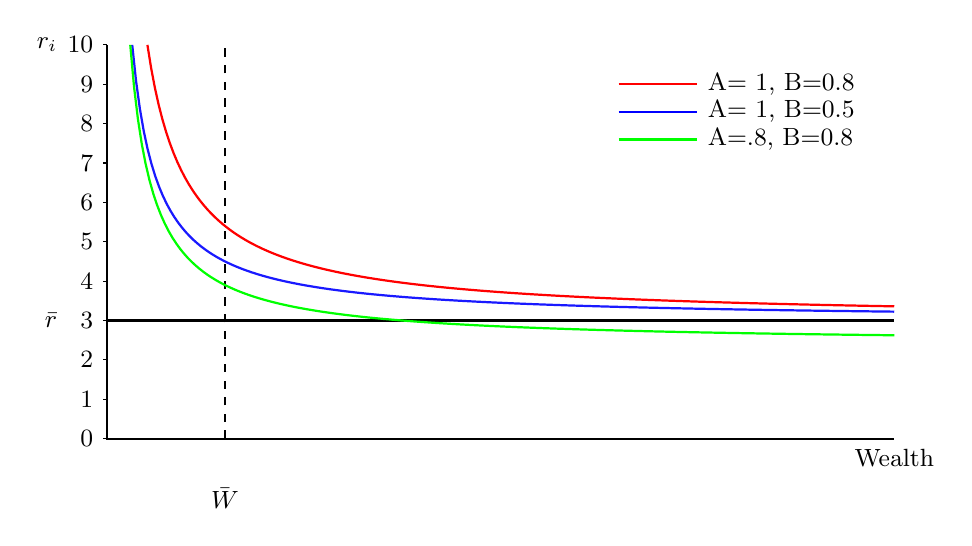
\begin{tikzpicture}[scale=.5]
%\def\bndmax{5}        %https://tex.stackexchange.com/questions/68462/filling-a-complex-region-with-tikz
%\def\bndmin{0.2}
\def \Y {10}  % height of y axis pecent
\def \W {20}  % length  of x axis
\def \Wbar {3} % jmeam wealth
\def \omega {3}
\def \A {1}  %was .5
\def \B {.5}
%Equation   \[ r_i = (A + .5 \frac{\bar{W}}{W_i})\omega\]
\def \Wmin{.63}  %This sets the lower limit fo the 
\def \Wmin{(\B*\Wbar)/(\Y/\omega-\A)} %function to keep in in bounds
	
\tikzset{func/.style={thick,color=blue!90}}	

\draw [thick] (0,\Y)node[left=.5cm]{$r_i$} -- (0,0)--(\W,0)node[below]{Wealth};  	% Axes
\draw [thick] (0,\omega)node[left=.5cm]{$\bar r$} -- (\W,\omega);  	% Axes
\draw [thick,dashed] ( \Wbar,0)node[below=.5cm]{$\bar{W}$} -- (\Wbar,\Y);  	% Axes

\foreach \yi in {0,...,\Y} \draw (0,\yi)--(-.1,\yi)node[left]{\small$\yi$};

\draw[func,domain=\Wmin:\W] plot [samples=200] (\x,{(\A+\B*\Wbar/\x)*\omega});
\def \A {.8}
\draw[func,domain=\Wmin:\W, green] plot [samples=200] (\x,{(\A+\B*\Wbar/\x)*\omega});

\def \A {1}
\def \B {.8}
\draw[func,domain=\Wmin:\W, red] plot [samples=200] (\x,{(\A+\B*\Wbar/\x)*\omega});

\draw [red,  thick](13, 9)--(15,9)node [right, black] {\small A=\ 1,\ B=0.8};
\draw [blue,  thick](13, 8.3)--(15,8.3)node [right, black] {\small A=\ 1,\ B=0.5};
\draw [green, thick](13, 7.6)--(15,7.6)node [right, black] {\small A=.8, B=0.8};
\end{tikzpicture}

% \caption{Hypothetical wealth-dependent borrowing cost}
% \label{Fig:BorrowingCost}
% \end{center}
% \end{figure}%

This has a number of immediate implications. First, if agents discount at their borrowing rate, wealthier agents a lower discount rate and therefore value properties more highly. 

Second, given the  common rule that mortgage payments cannot exceed some fraction of disposable income, the wealthy will be able borrow larger amounts and at lower interest rates that the less wealthy. At any distance from the centre they will be able to make a higher bid.
 
If the expected return on a property is greater than the individual cost of borrowing, it would pay any agent to borrow as much as possible and purchase properties as they become available.

\subsubsection{The rate of return on a property purchase $v$}
To explore the implication of the financialization of the urban land market we need a function to calculate the return on a unit of land that reflects the actual gradient of opportunity in financial markets. We begin with the price appreciation, $\Delta P=P_T-P_0 = (1+\dot p)P_0-P_0 $, where $\dot p$ is the rate of price appreciation over the period $T$. Rates will all be specified for the period $T$. Transaction costs, including real estate fees, take a fraction from the value of the final sale.

 The speculator invests a down payment, $D$, and gets back at time $T$ the  increased price $(1+\dot p)P_0$, plus rents, minus any costs and minus the mortgage with interest.
%footnote{We can include a use value, $U$ in place of rent for expatriate owners to represent using the property - say one month a year - when they are not renting the property and a \textbf{vacancy tax},
%$T$ at rate $t$ to affect the speculator's  decision.
 
The rate of return is the value of the gain, $V$,  over the size of the downpayment, $D$, where
\begin{equation}
V =capital\ gain - Interest\ due  	+ Rent  - operating\ cost\    
\end{equation}

The rate of return is $v = \frac{V}{D}$. 

Both the  share of the price  that can be mortgaged, $m$, and the interest rate  and $r$ may be functions of the agent's wealth. $\delta$ represents the net capital gains tax. It makes it possible to capture the capital gains kept. If it is set to one, it simplifies the equations, all is kept. Keeping the variable offers a policy variable to control the return on financial capital.

\begin{eqnarray*}
V  %	&=& capital\ gain - Interest\ due  	+ Rent  - operating\ cost\\
% 	&=& \delta P_T-D \qquad \qquad \quad - (1+\delta r)M \quad	 + R  	-C\\
% 	&=& \delta P _T \qquad-(P_0-M) \quad- (1+\delta r)M 	 + R  	-C\\
%	&=& \delta (1+\dot p)  P_0 -(P_O -M)  -(1+\delta r)mP_0  + R  -C\\
%	&=& \delta (1+\dot p)  P_0 -P_O + M \qquad -(1+\delta r)mP_0  + R -C\\
%	&=&( \delta (1+\dot p)-1)  P_0  + mP_0 \quad -(1+ \delta r)mP_0  + (\rho-\kappa)P_0\\	
%	&=& \left(  \delta (1+\dot p)-1    + m \quad - m(1+\delta r)  + (\rho-\kappa)\right)P_0\\'
%	&=& \left(  \delta (1+\dot p)-1    + m \quad - m-\delta rm  + (\rho-\kappa)\right)P_0\\
&=& \delta(P_T- (1+r)M) \qquad \qquad 	 + R  	-C   - T\\
&=& \delta((1+\dot p)  P_0- (1+r)mP_0)   + \rho P_0  	-\kappa P_0 - tP_0\\
&=&( \delta((1+\dot p)  - (1+r)m) \ + \rho   	-\kappa -t) P_0
\end{eqnarray*}

This is the  net present value of buying, and selling after one period. \textbf{It has  6 exogenous parameters}. Operating revenue and costs $ \rho -\kappa - t$ a present value. 

The rate of return is $v = \frac{V}{D}$. For expat investors, we get a \textbf{decision rule}:\begin{enumerate}
\item  if $v \geq a$ (with some private use?) with no rent,  don't bother renting. 
\item If $v(no\ rent\ and\ tax) < a\leq v(with\ rent)$,  then  rent. 
\item If $ v(with\ rent) \le a $,  then sell 
\end{enumerate}


We can, with some simplifications, write
\begin{eqnarray}
\frac{V}{D}&=&( \delta((1+\dot p)  - (1+r)m) \ + \rho   	-\kappa - t ) \frac{P_0}{D}   \nonumber\\
		&=&( \delta((1+\dot p)  - (1+r)m) \ + \rho   	-\kappa - t ) \frac{P_0}{P_0-mP_0}   \nonumber\\
		&=&\frac{ \delta(1+\dot p  - (1+r)m) \ + \rho   	-\kappa - t } {1-m} \label{Eqn:DecisionRule}
\end{eqnarray}

\subsubsection{Returns on capital are higher for wealthy investors}

\begin{figure}[htb]
\begin{center}

% Large version
% \begin{tikzpicture}[scale=.5]
% %\def\bndmax{5}        %https://tex.stackexchange.com/questions/68462/filling-a-complex-region-with-tikz
% %\def\bndmin{0.2}
% \def \Y {10}  % height of y axis pecent
% \def \W {20}  % length  of x axis
% \def \Wbar {3} % jmeam wealth
% \def \omega {3}
% \def \A {1}  %was .5
% \def \B {.5}
% %Equation   \[ r_i = (A + .5 \frac{\bar{W}}{W_i})\omega\]
% \def \Wmin{.63}  %This sets the lower limit fo the 
% \def \Wmin{(\B*\Wbar)/(\Y/\omega-\A)} %function to keep in in bounds
	
% \tikzset{func/.style={thick,color=blue!90}}	

% \draw [thick] (0,\Y)node[left=.5cm]{$r_i$} -- (0,0)--(\W,0)node[below]{Wealth};  	% Axes
% \draw [thick] (0,\omega)node[left=.5cm]{$\bar r$} -- (\W,\omega);  	% Axes
% \draw [thick,dashed] ( \Wbar,0)node[below=.5cm]{$\bar{W}$} -- (\Wbar,\Y);  	% Axes

% \foreach \yi in {0,...,\Y} \draw (0,\yi)--(-.1,\yi)node[left]{\small$\yi$};

% \draw[func,domain=\Wmin:\W] plot [samples=200] (\x,{(\A+\B*\Wbar/\x)*\omega});
% \def \A {.8}
% \draw[func,domain=\Wmin:\W, green] plot [samples=200] (\x,{(\A+\B*\Wbar/\x)*\omega});

% \def \A {1}
% \def \B {.8}
% \draw[func,domain=\Wmin:\W, red] plot [samples=200] (\x,{(\A+\B*\Wbar/\x)*\omega});

% \draw [red,  thick](13, 9)--(15,9)node [right, black] {\small A=\ 1,\ B=0.8};
% \draw [blue,  thick](13, 8.3)--(15,8.3)node [right, black] {\small A=\ 1,\ B=0.5};
% \draw [green, thick](13, 7.6)--(15,7.6)node [right, black] {\small A=.8, B=0.8};
% \end{tikzpicture}


\[   r^h=\frac{ \delta(1+\dot p  - (1+r)m) \ + \rho   	-\kappa - t } {1-m}    \]
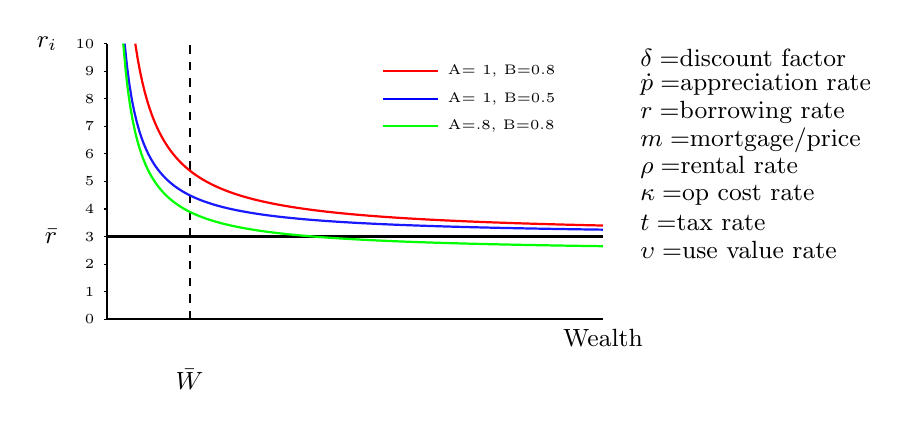
\begin{tikzpicture}[scale=.35]
%\def\bndmax{5}        %https://tex.stackexchange.com/questions/68462/filling-a-complex-region-with-tikz
%\def\bndmin{0.2}
\def \Y {10}  % height of y axis percent
\def \W {18}  % length  of x axis
\def \Wbar {3} % j mean wealth
\def \omega {3}
\def \A {1}  %was .5
\def \B {.5}
%Equation   \[ r_i = (A + .5 \frac{\bar{W}}{W_i})\omega\]
\def \Wmin{.63}  %This sets the lower limit fo the 
\def \Wmin{(\B*\Wbar)/(\Y/\omega-\A)} %function to keep in in bounds
	
\tikzset{func/.style={thick,color=blue!90}}	

\draw [thick] (0,\Y)node[left=.5cm]{$r_i$} -- (0,0)--(\W,0)node[below]{Wealth};  	% Axes
\draw [thick] (0,\omega)node[left=.5cm]{$\bar r$} -- (\W,\omega);  	% Axes
\draw [thick,dashed] ( \Wbar,0)node[below=.5cm]{$\bar{W}$} -- (\Wbar,\Y);  	% Axes

\foreach \yi in {0,...,\Y} \draw (0,\yi)--(-.1,\yi)node[left]{\tiny$\yi$};

\draw[func,domain=\Wmin:\W] plot [samples=200] (\x,{(\A+\B*\Wbar/\x)*\omega});
\def \A {.8}
\draw[func,domain=\Wmin:\W, green] plot [samples=200] (\x,{(\A+\B*\Wbar/\x)*\omega});

\def \A {1}
\def \B {.8}
\draw[func,domain=\Wmin:\W, red] plot [samples=200] (\x,{(\A+\B*\Wbar/\x)*\omega});

\draw [red,  thick](10, 9)--(12,9)node [right, black] {\tiny A=\ 1,\ B=0.8};
\draw [blue,  thick](10, 8)--(12,8)node [right, black] {\tiny A=\ 1,\ B=0.5};
\draw [green, thick](10, 7)--(12,7)node [right, black] {\tiny A=.8, B=0.8};

\def \W {19}  % length  of x axis
\node[right] at (\W,9.5){\small$\delta=$discount factor};
\node[right] at (\W,8.5){\small$\dot p=$appreciation rate};
\node[right] at (\W,7.5){\small$r=$borrowing rate};
\node[right] at (\W,6.5){\small$m=$mortgage/price};
\node[right] at (\W,5.5){\small$\rho=$rental  rate};
\node[right] at (\W,4.5){\small$\kappa=$op cost rate};
\node[right] at (\W,3.5){\small$t=$tax rate};
\node[right] at (\W,2.5){\small$\upsilon=$use value rate};
 \end{tikzpicture}


\caption{Hypothetical wealth-dependent borrowing cost}
\label{Fig:BorrowingCost}
\end{center}
\end{figure}%





\section{Where does this go? Space - describe model logic - VERY OLD DESCRIPTION}


Initialize the model with grid. Each element contains 1 housing unit.

The model space is divided into a uniform grid of single family homes % Additions: apartment buildings, a mechanism to subdivide homes, rent bedrooms, accumulate adjacent land and build new higher density buildings, an urban land boundary, a mechanism for wealth agglomeration through density.

%Household agents have:

\begin{enumerate}
   \item A home. Agents live somewhere, inside or outside the city,
   \item finances: they have assets, a housing budget, income, and a spending pattern
   # family lending pattern  
   shaped by profession, demographics, family structure, etc.) 
   # risk profile
   \item utility function: they have a utility function with location  preferences 
   # amenity, open space, house size requirements, transportation costs
   # shaped by profession, demographics, family structure, etc
\end{enumerate}	

 \subsection{External Capital}
 An investor that buys up assets that cross bellow some lower threshold (threshold is higher during speculative booms), or in consolidating regions.


\subsection{Model Steps - Housing market}


at every time step 
    1) Some new tenants arrive into the city
    
    2) All unhoused tenants look for a housing unit 
    
        a) They have to decide whether to buy or rent. Decision depends on their income, and the availability of Corporation of Public Housing loans 


        b) If they buy, they seek apartment and evaluate, and place a bid (see ALMA)
        
        c) if they rent, they look for an apartment that matches xyz criteria, and place request to rent. Rental is given by the landlord to the first tenant that matches the asking rental price. 


Workers give up their search and leave the city if they do not find a housing unit 



\chapter{Conclusion}


The economics is clear that this is what's at stake is productivity of cities, the distributive features of the economy and the impact of the middle class.

In a passage that can be seen as a direct precursor to our analysis of urban land rent, Ricardo  wrote in his 1817 Principles of Political Economy, %Early theorists like Ricardo described something can be thought of as describing a three-factor, three-class model with great precision but without the use of mathematics.   

Adding 2 things 1. rent extraction and 2. power law scaling of productivity, we find rent is the breaks on the engine of wealth creation

INTEGRATE- AS THIS SUGGEST ALL GOES TO LANDLOARDS?
What changes over time is the share that goes to each group:

As Ricardo said

\begin{quotation}   
 “The produce of the earth - all that is derived from its surface by the united application of labour, machinery, and capital, is divided among three classes of the community; namely, the proprietor of the land, the owner of the stock or capital necessary for its cultivation, and the labourers by whose industry it is cultivated. ...  But in different stages of society, the proportions of the whole produce of the earth which will be allotted to each of these classes, under the names of rent, profit, and wages, will be essentially different; ”  Chapter 1
\end{quotation}

what's changed is xyz

Ricardo was ``the first writer to take the industrial phenomenon of city life and to create an economy based upon those characteristics.''  \footnote{Simon N. Patten,  The Quarterly Journal of Economics, volume 7, Issue 3, April 1893, Pages 322–352, https://doi.org/10.2307/1884006 }  

Our focus is land rents, but in the context of an urban economy. 

{Ricardo concluded that % , ``It follows then, that 
``the interest of the landlord is always opposed to the interest of every other class in the community.'' }



%Strikingly, Ricardo concluded\footnote{An Essay on the Influence of a low Price of Corn} that, “It follows then, that the interest of the landlord is always opposed to the interest of every other class in the community.” Rents approriated by the land owner are not available to the worker  or the capitalist for re-investment. This is a view that Henry George would later pick up and it is one that we return to in our study, since the issue of urban rents is of great policy importance. 

\part{Implications: Systems Analysis, Interventions, and Policy}
\chapter{Methodology}

Methodological questions: 

    - agent models (integrating theory more completely into agent models)
    
    - rent theory

Core model

    - static version
    
    - dynamic version

Simulations

Result---> hysteresis

policy
\chapter{Resilience}

The model gives a resilience result which is that shared wealth through housing is not resilience.

It can also be used with a driven version of the model to show that the model pumps wealth out on the upswing and on the downswing - like a kind if ratchet.

\section{Resilience elements it gives insight into}

This section explores the resilience dynamics of distribution of wealth within a class of market models.  

Using a systems design approach and looking at resilience measures and alternative regimes gives insights into patterns of distribution and how that shapes wealth. 

The two significant concepts of resilience for this work are the relationship between distinct alternative regimes and patterns of cycling within a single regime. 

\section{What is resilience and how is it connected to this work}

Resilience is a concept that has to with the way in which a system resists disturbance or maintains identity through disturbance. The concept has emerged independently with different, but related definitions in various fields. 
There are a class of systems that this idea of resilience should be applicable or illuminating for, however the concepts and measures that exist already are ill-suited to the dynamics of the system. 
The work in this thesis draws from the measures from existing measures and concepts of resilience from various discipline to evolve a measure that can apply to this other class of systems. 

Shaping this c
ore broadly applicable concept that 
We can approach change in various systems using technical tools that are transferable. 
The concept 

\section{Resilience in engineering}

In Engineering, Resilience is defined as the return properties of a system. 
It is the measures relating to how a system comes back to its stable equilibrium or stable state. For example if you push a branch on a tree, it will oscillate and settle back to its resting position. 

Stability properties are important in engineering because engineers are responsible for signing off the performance of system, whether the the system is a bridge or a chemical reactant or an electrical circuit. Stability is an aspect of the system’s behaviour. The engineer needs measures to predict the stability of the system when it's perturbed. (Specific) 

Engineering resilience is distinct from the failure zones or the threshold of failure - for example the level of force/weight or number of stress cycles that would be required to collapse a bridge. While those measures pertain the thresholds beyond which the system would fail, resilience is about describing how the system recovers from perturbations that do not break it. 

The primary measure is how long the system takes to return to its equilibrium, i.e. the return time. (Equation) There are seven measures, listed in table XYZ that pertain to return to equilibrium properties.  (Table)

There is some variation in the use of the concept in specific disciplines of Engineering. For example, in transport engineering it has something to do with traffic flow.

\section{Resilience in ecology}

In Ecology resilience is defined as the way in which systems maintain identity through transformations. 

In engineering, the concept of resilience centres on the idea of a single equilibrium. If the system is not disturbed, it will stay at equilibrium and the resilience measures account for the system’s return to this equilibrium. In the ecology, on the other hand, instead of a single equilibrium the underlying pattern of the system has a dynamic structure. For example the ecosystem of a forest contains ongoing cycles of life and death and evolving patterns and interactions and yet sustains its identity as a forest. 

An ecosystem can experience big shocks or disturbances without losing its basic identity. For example, there can be drought, floods, fire, species loss, etc and the forest can recover and continue to be a forest. 
((The forest can regrow, one species might replace another and the forest changes but it doesn’t necessarily stop being a forest.)) But some disturbances can tip the ecosystem over into a different pattern of functioning. For example if the land is cleared and animals come into to graze the seedling trees so that they do not grow back, the forest can transition to a grassland ecosystem. Or if the region becomes dry enough, the forest can transition to become a desert. 

In ecology these alternative patterns of a system that may be identified as a forest, grassland, or desert are called regimes. In Ecological resilience studies, this concept of regimes replaces the simpler idea of equilibrium, differing both because the underlying pattern is more complex and because there are multiple regimes that the ecosystem of the same land can shift between. 

Part of what resilience in ecology is getting at, then, is what kind and how big the disruption can be before the ecosystem becomes a different kind of ecosystem. Resilience measures describe the properties of these distinct regimes and the relations between them. The most common measure is the size of the perturbation the system can withstand without transitioning into an alternative pattern of functioning or regime.  

This approach to resilience was introduced by C.S. Holling with his 1973 paper on a Spruce Budworm model of a forest ecosystem. In this paper he argued that there was an evolving interrelationship/feedback cycle between Spruce growth/regrowth and the population of Spruce Budworms that eat them. This interaction drove ongoing cycles of forest recovery and collapse. 

Holling’s work established the concept of these kinds of cycled and alternative regimes in ecosystems. Subsequent work by Marten Scheffer in lake eutrophication validated that alternative regimes appear in ecosystems in the real world. Now there is a database tracking thresholds and regime shifts in ecological systems with over a hundred entries showing its common.  ([https://www.resalliance.org/thresholds-db](https://www.resalliance.org/thresholds-db)) 

In ecology, this idea of resilience has evolved into a dynamic concept that is very important in climate change science and ecological conservation. Resilience measures show how a system maintains identity through change by measuring the relationship between regimes, that is how close a system is to transitioning to a different regime or pattern of functioning. Thus the concept of ecological resilience and alternate regimes give tools to understand what is possible for an ecosystem. This give insight both into how ecosystems can be preserved but also what happens when they transform. 


\section{Resilience in social systems}

The ecological concept of Resilience has since been applied widely to various systems across disciplines (*INSERT EXAMPLES*). Frances Westley applies Holling’s idea of alternative regimes to social systems as the basis for a theory of social innovation. 

Westley defines social innovation as “a change in the routines, resource flows, authority flows or beliefs in any social system.” According to Westley “a successful social innovation also has durability and broad impact.” 
Her studies in social innovation focus on how individuals, groups, or institutions are able to shift social systems to achieve certain goals. 

Westley’s research question is how social systems transform. This frame differs from the majority of resilience work in engineering and ecology because the focus there tends to be on maintaining the integrity of the system, whereas Westley’s work is focused on how to move between regimes. 

For example, in the Great Bear Rainforest in British Columbia in the late 1990’s (??) clearcutting for pulp and paper was threatening some of the last old old growth forests in the region and disrupting the lives of people who depended on them. Over years of unchecked logging combined with a history of land appropriation, there was ongoing local resistance. In 199X images of the devastation spread through international media and led to a boycott of paper products from clearcutting. This moment of crisis brought the forestry industry to the table. After a carefully structured process of conversation and engagement between community organizers, political leaders, and industry they put the Great Bear Rainforest under Indigenous community control. 

This change in governance structure can be understood social system that can be understood as a regime change because there were a set of patterns and feedbacks holding the old system in place and and there new set of patterns and feedbacks holding the new system in place. Each regime has a distinct pattern of functioning or identity. 

The idea of resilience in social innovation illuminates how the patterns of different regimes structure the social systems. What is different about the two regime in the case of the Great Bear Rainforest is the distribution of the flow of money and power - or the the language of social innovation, resources and authority. This changed the routines and habits of the people making up the social system as they became more directly involved in managing the forest. The result is that the ancient Great Bear Rainforest survived. 

The study of resilience within social innovation looks at how actors within  systems play a role in shaping transformation of interconnected social-ecological systems. Westley specifically studies individuals, groups, or institutions who have the intention to shift social systems to achieve certain goals. This means that there is a directed strategic nature to the agents. This is illustrated by the case of the Great Bear Rainforest by the different stakeholders from industry, community and governance who are are all actively working to achieve specific goals. However none of these actors are outside outside the system. Even those with power cannot completely control the system. Their efforts interact with the actions of others and the broader context of the whole

Social systems are dynamic. There is no fixed equilibrium and yet they have clusters of properties that persist and can prove difficult to change. These patterns with distinct identities are described in social innovation theory as regimes. These patterns can pertain to various feature, from the routines that structure interactions to resource flows within the system. In the example of the Great Bear Rainforest, under the previous system the resources and money flowed out of the community and decisions were made by distant corporations. The shift in governance structurally affected both the ecosystem and the culture of the communities. When they shifted to community governance, the emphasis shifted away from extraction and toward investing and building the forest and the community. (ADD CONCRETE DETAILS/NUMBERS?) 

Sometimes people can achieve their goals and sometimes they do not and it depend on both what they do and the state of the system. In her grounded theory work studying people who have attempted and succeeded in changing systems, Westley observed that sometimes there are moments of opportunity that make shifts in the system possible.  In the rainforest example, there were years of Indigenous organizing and building an environmental movement. 
The change became possible at a particular moment when commodity prices were placing pressure on the industry and coordination between local and national environmentalists resulting in international boycotts of pulp and paper products from clearcut forest, particularly across Europe. The indigenous organizers were able to achieve more in this moment of opportunity.

According to Westley a successful social innovation also “has durability and broad impact.” This is a description of the change but it also illuminates how the resilience concept of regimes is useful. One feature of systems is that a set of feedback loops will hold patterns of interactions, resources flows, etc in place. Many changes simply die out.  The changes that last do so because they change the flows and dynamics in ways that are held in place by new feedback loops.  Social Innovation theorists have used the concept of regimes to explain this phenomena. If the system state is perturbed enough another set of patterns can come to dominate.  (MAKE SURE THESE TERMS ALIGN WITH THE PRECISE TERMINOLOGY USED LATER) In the example, after the shift to the community governance that became self-reinforcing as different feedback loops emerged to structure the building of relationships and institutional structures, community habits, networks of support, and resource flows. 

\section{Role of this thesis}

What has been articulated in Social innovation theory is a story of how feedback loops hold the patterns in place  and how systems can switch between sets of patterns. Westley and others have applied the concept of resilience as an explanatory framework, rather than as a a precise mathematical statement. 
The thesis seeks to operationalize these concepts within a formal model in the context of social systems. 


- By operationalizing into this model, we can patterns in how systems shift between regimes. Specifically in this thesis the models show where in the systems there are opportunities - ie the system is more vulnerable or -open to change. 
- In practice regimes change can move you into a more or less desired state. Here I focus on opportunities and interventions. 
- Inventions are…
- By looking at where the system has opportunity to change this work illuminates how actors might be able to identify opportunities for regime change. 
- 











he analysis has been applied conceptually, rather than as a precise mathematical statement. Thus far, in the study of social innovation 

Routines, resource authority flow and beliefs. 

International concern
Boycotts 
Political movement

Effective local movement established an indigenously led sustainable forest and tenure
It 



Community leaders were able to establish a 




Social innovation involves interventions or actions 




She studies I

Change in technology and demand for wood. 

For example, she looks at how various countries responded to the AIDS crisis and how activists in certain shaped 

There’s a debate about how systems transform. 
Impersonal forces of history like the development of agriculture
She’s studying the phenomena of change in order to inform 
The research is about how people try to change the word. 

(ie. a system consisting of different interconnected entities such as  individuals, groups, and institutions relating to each other and forming a whole.)

An interdependence of a social and cultural element 

Series of interrelationships between individuals and groups and institutions forming a whole. 



% [[adaptive cycle]]
\chapter{Interventions - TO ADD}

There is a housing crisis with rapidly increasing cost of living as a result of rising housing prices. 
In the last few years, the need for affordable housing has come into focus as one of the most pressing issues facing Canadians. As more and more Canadians are finding housing unaffordable, the effects are being seen across the board in everything from declining homeownership rates to increasing numbers of Canadians unable to afford housing at all.

...

In principle there are a range of alternative regimes.
The advantages of financial capital have multiple sources, so the result does not require that any one advantage be true all of the time, so it's not sensitive to small or localized changes in policy environments. The analysis tells us that the advantages of financialized capital are robust.

are true across a range of explanations/features - including REITS and formal financial capital, second houses purchased by the investment vehicles by the middle class, and mortgages which represents the banks' share of privately owned homes


...


In the last few years, the need for affordable housing has come into focus as one of the most pressing issues facing Canadians. As more and more Canadians are finding housing unaffordable, the effects are being seen across the board in everything from declining homeownership rates to increasing numbers of Canadians unable to afford housing at all.

Over the course of two years of studying how changes in the housing market affect housing affordability, Social Innovation Canada has emerged with a picture of a system at a historic tipping point. 

This crisis means that we now have a huge but brief window of opportunity to fix the housing system.  Due to this current crisis, the government has moved to establish a National Housing Strategy and make massive investment in housing. This creates the opportunity for profound and lasting change, but unless steps are taken to address the drivers that have led to the crisis, the housing market will likely continue on its trajectory of eroding the middle class and making vulnerable populations worse off.   

This crisis has been developing for years. Canada's housing market reached an important turning point between the 2011 and 2016 census: homeownership rates both nationally and across major cities fell for the first time on record and the roots of this shocking reversal in housing trends goes back to 1993 when the federal government froze federal funding to new public housing projects, transferring public housing authority to provincial, municipal, and local governments. 

From the end of WWII until this point, Canada’s housing strategy ensured housing accessibility and affordability via a growing stock of public housing and cooperatives. These were funded by xx and made home ownership increasingly accessible and affordable. By the 1990s, this post-war housing strategy had built a prosperous and productive home-owning middle class: almost 70% of households were homeowners. 

In 1993, without federal leadership and funds, the social housing sector stalled, setting the Canadian housing market on the path to the current crisis. However, we didn’t see the true effect on homeownership until later because interest rates were dropping in the same period. This meant that home ownership continued to grow despite rising prices and slow growth in real wages. According to the International Monetary Fund and CMHC, these falling interest rates can explain the majority of the growth in house prices relative to incomes in most Canadian cities during this period. 

Meanwhile, low returns for investors in other sectors and rising home prices drove investors into the housing market. Speculative demand drove already rising home prices up further and faster rising prices attracted more speculative investment. Private capital began to take over the housing stock. This is the heart of the process called financialization. 

This trajectory of the market is preventing an increasing number of people in Canada from accessing safe and affordable homes. If financialization proceeds to its logical limit, the home-owning middle class will shrink, vulnerable populations will get poorer and financial institutions will extract more and more value from our cities.

However, real and lasting change can be made through a multi-pronged approach that includes innovative ownership models such as shared equity, co-housing and community land trusts; innovative financial models, products and services geared towards affordable housing; and greater alignment between municipal, provincial and federal programs with affordable housing developers and providers, investors and financial institutions to facilitate the creation of affordable housing units.

SI Canada proposes to establish a fund with a layer of concessionary funding to support deep, perpetual affordability. This could be part of a larger strategy to bring together stakeholders including government, non-profit, incubators, housing developers, community members, and financial institutions to take successful models that have emerged through the national housing strategy and scale them to make them the new normal. This  “all-hands-on-deck” approach brings together all the actors required to act quickly and effectively to design and implement solutions to problems that neither the government, the market or civil society are able to solve alone.  

This housing crisis could be the moment that Canada gets housing right. For a brief moment Canada has an opportunity to change the trajectory of housing affordability in Canada forever.


\section{Systems change}


%[[Nash asumption that everybody else will keep doing what they're doing]]
Bichiari cooperation
like to be somewhere else, like everyone else to make the adjustment at the same time. .

these system have feedback loops with the switching- the circuit resources creates more of itself-- the part's fo the land the water flows deepens the stream - making it more resilient, possibly wearing it out. - a kind of autopoetic quality -

switch is formally like a transistor/switch- also like a kind of tai chi - it has to use the energy of the particular kind of force coming in which is itself directed/complex/ has a mind, and direct that into the new system-- the input and the switch are complex systems and systems with minds.


the reductions to systems models become more not less important in the presence of this richness/complexity because it matters to desegregate the dynamics and the universal patterns of the type


\section{Social engineering}

has to relinqish it's commitment to state. 


\section{Who gets what share?}

As Ricardo said
\begin{quotation}   
 “The produce of the earth - all that is derived from its surface by the united application of labour, machinery, and capital, is divided among three classes of the community; namely, the proprietor of the land, the owner of the stock or capital necessary for its cultivation, and the labourers by whose industry it is cultivated. ...  But in different stages of society, the proportions of the whole produce of the earth which will be allotted to each of these classes, under the names of rent, profit, and wages, will be essentially different; ”  Chapter 1
\end{quotation}

% What changes over time is the share that goes to each group

That's what's at stake here.
The concern of the classical economists is central again, and we have the theoretical tools, to formalize the understanding.

We also have examples from many efforts to shift the patterns towards shared wealth to draw on. 

What are the prospects for this moment?

\begin{comment}
TODO

- Get rent_and_growth from notes_and_references
- Check we got intro from TeXnicle
- Get notation from TeXnicle or overleaf
- Check - excess return on urban capital
- Check - amenity/financialized returns
- Get ODD protocol..

- Edit and put in the notes on methods from TeXnicle

- get Draft Scale  chapter 8 from TeXnicle

- Get tix diagrams in Overleaf - make series to see the plots and identify gaps

- Glossary and symbols pages
- Index
- Move figures into seperate files, ideally one file per series, edit figrues
- Bibliography
- Website up

\end{comment}